
%% bare_jrnl.tex
%% V1.3
%% 2007/01/11
%% by Michael Shell
%% see http://www.michaelshell.org/
%% for current contact information.
%%
%% This is a skeleton file demonstrating the use of IEEEtran.cls
%% (requires IEEEtran.cls version 1.7 or later) with an IEEE journal paper.
%%
%% Support sites:
%% http://www.michaelshell.org/tex/ieeetran/
%% http://www.ctan.org/tex-archive/macros/latex/contrib/IEEEtran/
%% and
%% http://www.ieee.org/



% *** Authors should verify (and, if needed, correct) their LaTeX system  ***
% *** with the testflow diagnostic prior to trusting their LaTeX platform ***
% *** with production work. IEEE's font choices can trigger bugs that do  ***
% *** not appear when using other class files.                            ***
% The testflow support page is at:
% http://www.michaelshell.org/tex/testflow/


%%*************************************************************************
%% Legal Notice:
%% This code is offered as-is without any warranty either expressed or
%% implied; without even the implied warranty of MERCHANTABILITY or
%% FITNESS FOR A PARTICULAR PURPOSE! 
%% User assumes all risk.
%% In no event shall IEEE or any contributor to this code be liable for
%% any damages or losses, including, but not limited to, incidental,
%% consequential, or any other damages, resulting from the use or misuse
%% of any information contained here.
%%
%% All comments are the opinions of their respective authors and are not
%% necessarily endorsed by the IEEE.
%%
%% This work is distributed under the LaTeX Project Public License (LPPL)
%% ( http://www.latex-project.org/ ) version 1.3, and may be freely used,
%% distributed and modified. A copy of the LPPL, version 1.3, is included
%% in the base LaTeX documentation of all distributions of LaTeX released
%% 2003/12/01 or later.
%% Retain all contribution notices and credits.
%% ** Modified files should be clearly indicated as such, including  **
%% ** renaming them and changing author support contact information. **
%%
%% File list of work: IEEEtran.cls, IEEEtran_HOWTO.pdf, bare_adv.tex,
%%                    bare_conf.tex, bare_jrnl.tex, bare_jrnl_compsoc.tex
%%*************************************************************************

% Note that the a4paper option is mainly intended so that authors in
% countries using A4 can easily print to A4 and see how their papers will
% look in print - the typesetting of the document will not typically be
% affected with changes in paper size (but the bottom and side margins will).
% Use the testflow package mentioned above to verify correct handling of
% both paper sizes by the user's LaTeX system.
%
% Also note that the "draftcls" or "draftclsnofoot", not "draft", option
% should be used if it is desired that the figures are to be displayed in
% draft mode.
%
\documentclass[journal]{IEEEtran}
%
% If IEEEtran.cls has not been installed into the LaTeX system files,
% manually specify the path to it like:
% \documentclass[journal]{../sty/IEEEtran}





% Some very useful LaTeX packages include:
% (uncomment the ones you want to load)


% *** MISC UTILITY PACKAGES ***
%
%\usepackage{ifpdf}
% Heiko Oberdiek's ifpdf.sty is very useful if you need conditional
% compilation based on whether the output is pdf or dvi.
% usage:
% \ifpdf
%   % pdf code
% \else
%   % dvi code
% \fi
% The latest version of ifpdf.sty can be obtained from:
% http://www.ctan.org/tex-archive/macros/latex/contrib/oberdiek/
% Also, note that IEEEtran.cls V1.7 and later provides a builtin
% \ifCLASSINFOpdf conditional that works the same way.
% When switching from latex to pdflatex and vice-versa, the compiler may
% have to be run twice to clear warning/error messages.






% *** CITATION PACKAGES ***
%
%\usepackage{cite}
% cite.sty was written by Donald Arseneau
% V1.6 and later of IEEEtran pre-defines the format of the cite.sty package
% \cite{} output to follow that of IEEE. Loading the cite package will
% result in citation numbers being automatically sorted and properly
% "compressed/ranged". e.g., [1], [9], [2], [7], [5], [6] without using
% cite.sty will become [1], [2], [5]--[7], [9] using cite.sty. cite.sty's
% \cite will automatically add leading space, if needed. Use cite.sty's
% noadjust option (cite.sty V3.8 and later) if you want to turn this off.
% cite.sty is already installed on most LaTeX systems. Be sure and use
% version 4.0 (2003-05-27) and later if using hyperref.sty. cite.sty does
% not currently provide for hyperlinked citations.
% The latest version can be obtained at:
% http://www.ctan.org/tex-archive/macros/latex/contrib/cite/
% The documentation is contained in the cite.sty file itself.






% *** GRAPHICS RELATED PACKAGES ***
%
\ifCLASSINFOpdf
  % \usepackage[pdftex]{graphicx}
  % declare the path(s) where your graphic files are
  % \graphicspath{{../pdf/}{../jpeg/}}
  % and their extensions so you won't have to specify these with
  % every instance of \includegraphics
  % \DeclareGraphicsExtensions{.pdf,.jpeg,.png}
\else
  % or other class option (dvipsone, dvipdf, if not using dvips). graphicx
  % will default to the driver specified in the system graphics.cfg if no
  % driver is specified.
  % \usepackage[dvips]{graphicx}
  % declare the path(s) where your graphic files are
  % \graphicspath{{../eps/}}
  % and their extensions so you won't have to specify these with
  % every instance of \includegraphics
  % \DeclareGraphicsExtensions{.eps}
\fi
% graphicx was written by David Carlisle and Sebastian Rahtz. It is
% required if you want graphics, photos, etc. graphicx.sty is already
% installed on most LaTeX systems. The latest version and documentation can
% be obtained at: 
% http://www.ctan.org/tex-archive/macros/latex/required/graphics/
% Another good source of documentation is "Using Imported Graphics in
% LaTeX2e" by Keith Reckdahl which can be found as epslatex.ps or
% epslatex.pdf at: http://www.ctan.org/tex-archive/info/
%
% latex, and pdflatex in dvi mode, support graphics in encapsulated
% postscript (.eps) format. pdflatex in pdf mode supports graphics
% in .pdf, .jpeg, .png and .mps (metapost) formats. Users should ensure
% that all non-photo figures use a vector format (.eps, .pdf, .mps) and
% not a bitmapped formats (.jpeg, .png). IEEE frowns on bitmapped formats
% which can result in "jaggedy"/blurry rendering of lines and letters as
% well as large increases in file sizes.
%
% You can find documentation about the pdfTeX application at:
% http://www.tug.org/applications/pdftex





% *** MATH PACKAGES ***
%
\usepackage[cmex10]{amsmath}
% A popular package from the American Mathematical Society that provides
% many useful and powerful commands for dealing with mathematics. If using
% it, be sure to load this package with the cmex10 option to ensure that
% only type 1 fonts will utilized at all point sizes. Without this option,
% it is possible that some math symbols, particularly those within
% footnotes, will be rendered in bitmap form which will result in a
% document that can not be IEEE Xplore compliant!
%
% Also, note that the amsmath package sets \interdisplaylinepenalty to 10000
% thus preventing page breaks from occurring within multiline equations. Use:
%\interdisplaylinepenalty=2500
% after loading amsmath to restore such page breaks as IEEEtran.cls normally
% does. amsmath.sty is already installed on most LaTeX systems. The latest
% version and documentation can be obtained at:
% http://www.ctan.org/tex-archive/macros/latex/required/amslatex/math/





% *** SPECIALIZED LIST PACKAGES ***
%
%\usepackage{algorithmic}
% algorithmic.sty was written by Peter Williams and Rogerio Brito.
% This package provides an algorithmic environment fo describing algorithms.
% You can use the algorithmic environment in-text or within a figure
% environment to provide for a floating algorithm. Do NOT use the algorithm
% floating environment provided by algorithm.sty (by the same authors) or
% algorithm2e.sty (by Christophe Fiorio) as IEEE does not use dedicated
% algorithm float types and packages that provide these will not provide
% correct IEEE style captions. The latest version and documentation of
% algorithmic.sty can be obtained at:
% http://www.ctan.org/tex-archive/macros/latex/contrib/algorithms/
% There is also a support site at:
% http://algorithms.berlios.de/index.html
% Also of interest may be the (relatively newer and more customizable)
% algorithmicx.sty package by Szasz Janos:
% http://www.ctan.org/tex-archive/macros/latex/contrib/algorithmicx/




% *** ALIGNMENT PACKAGES ***
%
%\usepackage{array}
% Frank Mittelbach's and David Carlisle's array.sty patches and improves
% the standard LaTeX2e array and tabular environments to provide better
% appearance and additional user controls. As the default LaTeX2e table
% generation code is lacking to the point of almost being broken with
% respect to the quality of the end results, all users are strongly
% advised to use an enhanced (at the very least that provided by array.sty)
% set of table tools. array.sty is already installed on most systems. The
% latest version and documentation can be obtained at:
% http://www.ctan.org/tex-archive/macros/latex/required/tools/


%\usepackage{mdwmath}
%\usepackage{mdwtab}
% Also highly recommended is Mark Wooding's extremely powerful MDW tools,
% especially mdwmath.sty and mdwtab.sty which are used to format equations
% and tables, respectively. The MDWtools set is already installed on most
% LaTeX systems. The lastest version and documentation is available at:
% http://www.ctan.org/tex-archive/macros/latex/contrib/mdwtools/


% IEEEtran contains the IEEEeqnarray family of commands that can be used to
% generate multiline equations as well as matrices, tables, etc., of high
% quality.


%\usepackage{eqparbox}
% Also of notable interest is Scott Pakin's eqparbox package for creating
% (automatically sized) equal width boxes - aka "natural width parboxes".
% Available at:
% http://www.ctan.org/tex-archive/macros/latex/contrib/eqparbox/





% *** SUBFIGURE PACKAGES ***
%\usepackage[tight,footnotesize]{subfigure}
% subfigure.sty was written by Steven Douglas Cochran. This package makes it
% easy to put subfigures in your figures. e.g., "Figure 1a and 1b". For IEEE
% work, it is a good idea to load it with the tight package option to reduce
% the amount of white space around the subfigures. subfigure.sty is already
% installed on most LaTeX systems. The latest version and documentation can
% be obtained at:
% http://www.ctan.org/tex-archive/obsolete/macros/latex/contrib/subfigure/
% subfigure.sty has been superceeded by subfig.sty.



%\usepackage[caption=false]{caption}
%\usepackage[font=footnotesize]{subfig}
% subfig.sty, also written by Steven Douglas Cochran, is the modern
% replacement for subfigure.sty. However, subfig.sty requires and
% automatically loads Axel Sommerfeldt's caption.sty which will override
% IEEEtran.cls handling of captions and this will result in nonIEEE style
% figure/table captions. To prevent this problem, be sure and preload
% caption.sty with its "caption=false" package option. This is will preserve
% IEEEtran.cls handing of captions. Version 1.3 (2005/06/28) and later 
% (recommended due to many improvements over 1.2) of subfig.sty supports
% the caption=false option directly:
%\usepackage[caption=false,font=footnotesize]{subfig}
%
% The latest version and documentation can be obtained at:
% http://www.ctan.org/tex-archive/macros/latex/contrib/subfig/
% The latest version and documentation of caption.sty can be obtained at:
% http://www.ctan.org/tex-archive/macros/latex/contrib/caption/




% *** FLOAT PACKAGES ***
%
%\usepackage{fixltx2e}
% fixltx2e, the successor to the earlier fix2col.sty, was written by
% Frank Mittelbach and David Carlisle. This package corrects a few problems
% in the LaTeX2e kernel, the most notable of which is that in current
% LaTeX2e releases, the ordering of single and double column floats is not
% guaranteed to be preserved. Thus, an unpatched LaTeX2e can allow a
% single column figure to be placed prior to an earlier double column
% figure. The latest version and documentation can be found at:
% http://www.ctan.org/tex-archive/macros/latex/base/



%\usepackage{stfloats}
% stfloats.sty was written by Sigitas Tolusis. This package gives LaTeX2e
% the ability to do double column floats at the bottom of the page as well
% as the top. (e.g., "\begin{figure*}[!b]" is not normally possible in
% LaTeX2e). It also provides a command:
%\fnbelowfloat
% to enable the placement of footnotes below bottom floats (the standard
% LaTeX2e kernel puts them above bottom floats). This is an invasive package
% which rewrites many portions of the LaTeX2e float routines. It may not work
% with other packages that modify the LaTeX2e float routines. The latest
% version and documentation can be obtained at:
% http://www.ctan.org/tex-archive/macros/latex/contrib/sttools/
% Documentation is contained in the stfloats.sty comments as well as in the
% presfull.pdf file. Do not use the stfloats baselinefloat ability as IEEE
% does not allow \baselineskip to stretch. Authors submitting work to the
% IEEE should note that IEEE rarely uses double column equations and
% that authors should try to avoid such use. Do not be tempted to use the
% cuted.sty or midfloat.sty packages (also by Sigitas Tolusis) as IEEE does
% not format its papers in such ways.


%\ifCLASSOPTIONcaptionsoff
%  \usepackage[nomarkers]{endfloat}
% \let\MYoriglatexcaption\caption
% \renewcommand{\caption}[2][\relax]{\MYoriglatexcaption[#2]{#2}}
%\fi
% endfloat.sty was written by James Darrell McCauley and Jeff Goldberg.
% This package may be useful when used in conjunction with IEEEtran.cls'
% captionsoff option. Some IEEE journals/societies require that submissions
% have lists of figures/tables at the end of the paper and that
% figures/tables without any captions are placed on a page by themselves at
% the end of the document. If needed, the draftcls IEEEtran class option or
% \CLASSINPUTbaselinestretch interface can be used to increase the line
% spacing as well. Be sure and use the nomarkers option of endfloat to
% prevent endfloat from "marking" where the figures would have been placed
% in the text. The two hack lines of code above are a slight modification of
% that suggested by in the endfloat docs (section 8.3.1) to ensure that
% the full captions always appear in the list of figures/tables - even if
% the user used the short optional argument of \caption[]{}.
% IEEE papers do not typically make use of \caption[]'s optional argument,
% so this should not be an issue. A similar trick can be used to disable
% captions of packages such as subfig.sty that lack options to turn off
% the subcaptions:
% For subfig.sty:
% \let\MYorigsubfloat\subfloat
% \renewcommand{\subfloat}[2][\relax]{\MYorigsubfloat[]{#2}}
% For subfigure.sty:
% \let\MYorigsubfigure\subfigure
% \renewcommand{\subfigure}[2][\relax]{\MYorigsubfigure[]{#2}}
% However, the above trick will not work if both optional arguments of
% the \subfloat/subfig command are used. Furthermore, there needs to be a
% description of each subfigure *somewhere* and endfloat does not add
% subfigure captions to its list of figures. Thus, the best approach is to
% avoid the use of subfigure captions (many IEEE journals avoid them anyway)
% and instead reference/explain all the subfigures within the main caption.
% The latest version of endfloat.sty and its documentation can obtained at:
% http://www.ctan.org/tex-archive/macros/latex/contrib/endfloat/
%
% The IEEEtran \ifCLASSOPTIONcaptionsoff conditional can also be used
% later in the document, say, to conditionally put the References on a 
% page by themselves.


\usepackage{xspace}
\usepackage{textcase}

% Graphics
\usepackage{wasysym}
\usepackage{graphics}
\usepackage{graphicx}   % A package to allow insertion of
                        % external image files

\usepackage{comment}
\usepackage{amsfonts}
\usepackage{array}
\usepackage{booktabs}
\usepackage{capt-of}
\usepackage{colortbl}
\usepackage{graphicx}
\usepackage{multirow}
\usepackage{subfig}
\usepackage{pifont}
\usepackage[latin1]{inputenc}
\usepackage{times}
\usepackage{url}
\usepackage{boxedminipage}
\usepackage{xspace}
\usepackage{sepnum}
\usepackage{cite}
\usepackage{fancyhdr}

\usepackage{verbatim}
\usepackage{float}
\usepackage{tabularx}
\usepackage{calc}


\usepackage{rotating}


\usepackage{tikz}


% *** PDF, URL AND HYPERLINK PACKAGES ***
%
%\usepackage{url}
% url.sty was written by Donald Arseneau. It provides better support for
% handling and breaking URLs. url.sty is already installed on most LaTeX
% systems. The latest version can be obtained at:
% http://www.ctan.org/tex-archive/macros/latex/contrib/misc/
% Read the url.sty source comments for usage information. Basically,
% \url{my_url_here}.


\usepackage{url}


% *** Do not adjust lengths that control margins, column widths, etc. ***
% *** Do not use packages that alter fonts (such as pslatex).         ***
% There should be no need to do such things with IEEEtran.cls V1.6 and later.
% (Unless specifically asked to do so by the journal or conference you plan
% to submit to, of course. )

\floatstyle{ruled}
\newfloat{placeholder}{thp}{lop}
\floatname{placeholder}{Box}

\newcommand\error{\texttt{ERROR}}
\newcommand\ok{\texttt{OK}}


% correct bad hyphenation here
\hyphenation{op-tical net-works semi-conduc-tor}


\begin{document}
%
% paper title
% can use linebreaks \\ within to get better formatting as desired
\title{Thesis Journal Version}
%
%
% author names and IEEE memberships
% note positions of commas and nonbreaking spaces ( ~ ) LaTeX will not break
% a structure at a ~ so this keeps an author's name from being broken across
% two lines.
% use \thanks{} to gain access to the first footnote area
% a separate \thanks must be used for each paragraph as LaTeX2e's \thanks
% was not built to handle multiple paragraphs
%

\author{Adrian Schr{\"o}ter,~\IEEEmembership{Member,~IEEE}
        and~Daniela~Damian,~\IEEEmembership{Member,~IEEE}% <-this % stops a space
        }

% note the % following the last \IEEEmembership and also \thanks - 
% these prevent an unwanted space from occurring between the last author name
% and the end of the author line. i.e., if you had this:
% 
% \author{....lastname \thanks{...} \thanks{...} }
%                     ^------------^------------^----Do not want these spaces!
%
% a space would be appended to the last name and could cause every name on that
% line to be shifted left slightly. This is one of those "LaTeX things". For
% instance, "\textbf{A} \textbf{B}" will typeset as "A B" not "AB". To get
% "AB" then you have to do: "\textbf{A}\textbf{B}"
% \thanks is no different in this regard, so shield the last } of each \thanks
% that ends a line with a % and do not let a space in before the next \thanks.
% Spaces after \IEEEmembership other than the last one are OK (and needed) as
% you are supposed to have spaces between the names. For what it is worth,
% this is a minor point as most people would not even notice if the said evil
% space somehow managed to creep in.



% The paper headers
\markboth{Journal of \LaTeX\ Class Files,~Vol.~6, No.~1, January~2007}%
{Shell \MakeLowercase{\textit{et al.}}: Bare Demo of IEEEtran.cls for Journals}
% The only time the second header will appear is for the odd numbered pages
% after the title page when using the twoside option.
% 
% *** Note that you probably will NOT want to include the author's ***
% *** name in the headers of peer review papers.                   ***
% You can use \ifCLASSOPTIONpeerreview for conditional compilation here if
% you desire.




% If you want to put a publisher's ID mark on the page you can do it like
% this:
%\IEEEpubid{0000--0000/00\$00.00~\copyright~2007 IEEE}
% Remember, if you use this you must call \IEEEpubidadjcol in the second
% column for its text to clear the IEEEpubid mark.



% use for special paper notices
%\IEEEspecialpapernotice{(Invited Paper)}




% make the title area
\maketitle


\begin{abstract}
Efficient coordination among software developers is one key aspect in producing high quality software on time and on budget.
Many factors such as team distribution or the structure of the organization developing the software can increase the level of difficulty in coordination.
However, the problem runs deeper, it is often unclear which developers should coordinate their work.
%
We propose to leverage the concept of socio-technical congruence (which contrasts coordination needs with actual coordination) to improve the social interactions among developers 
by developing an approach and its implementation into a recommender system that identifies relevant coordinators.
Our unit of analysis is the integration build whose outcome represents the quality of coordination.
We developed and applied an approach in a number of case studies of the IBM Rational Team Concert development team.
%
As each software product is just the latest integration build ensuring a failure free build is of utmost importance to industry.
While developing an approach to improve coordination among software developers, we uncovered that unmet coordination needs as well as the communication structure in a team significantly influence build outcome.
\end{abstract}
% IEEEtran.cls defaults to using nonbold math in the Abstract.
% This preserves the distinction between vectors and scalars. However,
% if the journal you are submitting to favors bold math in the abstract,
% then you can use LaTeX's standard command \boldmath at the very start
% of the abstract to achieve this. Many IEEE journals frown on math
% in the abstract anyway.

% Note that keywords are not normally used for peerreview papers.
\begin{IEEEkeywords}
IEEEtran, journal, \LaTeX, paper, template.
\end{IEEEkeywords}






% For peer review papers, you can put extra information on the cover
% page as needed:
% \ifCLASSOPTIONpeerreview
% \begin{center} \bfseries EDICS Category: 3-BBND \end{center}
% \fi
%
% For peerreview papers, this IEEEtran command inserts a page break and
% creates the second title. It will be ignored for other modes.
\IEEEpeerreviewmaketitle



% !TEX root = thesis-journal.tex
\section{Introduction}
The software industry often visible through some of big companies such as Microsoft, Google, IBM, Dell, Apple, Oracle, and SAP represent several hundred billion US Dollars of profit a year. 
For example the software industry in USA in 2002 was producing according to the US Census a total revenue of 103.7 billion USD\footnote{http://www.census.gov/prod/ec02/ec0251i06.pdf last visited May 10th, 2012}.
As many engineering companies those companies in the software industry strive to optimize their engineering processes to produce software of higher quality in less time.

Software engineering researchers all over the world have dedicated countless hours to improve the way software is developed.
Several fields some not directly aimed at increasing productivity such as developing better programming languages~\cite{conf:prog:lang}, smarter compilers~\cite{cong:comp:constr}, and better educationial methods to teach algorithms and data structures~\cite{conf:sigcse} contribute indirectly.
Other fields are more directly interested in productivity, among them are research in software processes~\cite{conf:icssp}, effort estimation~\cite{molkken:isese:2003,boehm:analse:2000}, and software failure prediction~\cite{conf:promise}.

The vast body of knowledge accumulated to improve the software engineering process is strongly biased towards analyzing the technical side: supporting coding activities (e.g.~\cite{bassil:iwpc:2001,mens:tse:2004}) and analyzing source code to improve quality~\cite{zimmermann:oopsla:2005,nagappan:icse:2006}. 
Since producing source code is the main objective of software developer optimizing the coding aspect~\cite{bassil:iwpc:2001,mens:tse:2004} as well as analyzing the produced code for issues~\cite{nagappan:icse:2005,schroeter:isese:2006} lies at hand.

Others have focused on the people that produce the code. Studying their behaviour around coding activities~\cite{latoza:icse:2006}, how they communicate~\cite{ko:icse:2007,gopal:2002:comacm}, and how developer relations relate to productivity~\cite{gopal:2002:comacm} and quality~\cite{abreu:iwpse:2009,wolf:icse:2009}.
As in the former case there is much merit in focusing on the developer in the end she implements the features a software consists of and she inevitably introduces errors to the code base.

Both avenues, studying the human aspect and studying the technical aspect, yielded many useful results.
For example, on the human side, the organizational distance between developer is a good predictor of failure on file level~\cite{nagappan:icse:2008}, and on the technical side similar changes timely close are a good failure predictor~\cite{kim:icse:2007}.

Yet, to truly be able to optimize the software engineering process a more holistic view is needed that marries both the technical and social aspects.
One such way to marry those two aspects that as Conway stated are influencing each other~\cite{conway:datamination:1968} is to use the concept of socio-technical congruence in software engineering first formalized by Cataldo et al~\cite{cataldo:cscw:2006}.
They proposed to overlay networks constructed from social (who communicates with whom) and technical (whose code depends on whose source code) dependencies to get an overview of a projects social and technical interdependencies and derive insight through the miss-match between those two networks.

%%%%%%%%%%
%%%%%%%%%%
% removed stuff here
%%%%%%%%%%
%%%%%%%%%%


% some of the findings as a teaser
Socio-technical congruence forms a great basis to leverage several digitally recorded data treasures to generate useful and actionable information.
Patterns of developer pairs showed that there are developers when not talking to each other yet sharing a technical dependency endangered the upcoming software build.
Furthermore, we found in a student project that certain issues experienced during development can be traced back to code dependencies that could have been detected in real time.

% the two top level research questions
To complement the research that studied the relationship between socio-technical congruence and performance, we focus on build outcome as a metric for software quality.
Although build outcome is rarely considered when studying software quality, as it a course measure that often indicates multiple issues rather than a single specific one, studying build outcome is important as build success is fundamental in creating a product that can be shipped to a customer.
Often a successful build indicates that not only all test cases deemed important passed, a successful build towards the end of the release cycle often is the only indicator of customer acceptance with respect to requested features and their stability.
Furthermore, A failed build, on the other hand, demotivates software developers \cite{holck2004,damian:icgse:2007} and destabilizes the product \cite{cusumano1997}.
Hence, build success is of utmost importance to a business as it forms the very product the business hopes to sell.
%Therefore the two guiding research questions we address in this thesis to investigate whether socio-technical congruence can be used to generate actionable knowledge that can increase build success are:
%\begin{description}
%\item[RQ 1:] Does Socio-Technical Congruence influence build success?
%\item[RQ 2:] Can Socio-Technical Networks be leverage to generate recommendations to improve build success?
%\end{description}
%
%% methodology overview
%We are using a mixed methods approach to explore these two research questions.
%For \textbf{RQ~1} we employ data mining techniques by studying the artifacts such as task discussions and source code changes of a large industrial software project.
%The second research question (\textbf{RQ~2}) requires both quantitative and qualitative analysis methods.
%To find statistically relevant recommendations we employ data mining techniques, but to explore the usefulness and acceptance of such recommendations we make use of questionnaires, interviews, and observational studies.

























% !TEX root = thesis-journal.tex
\section{Background}
\label{chap:bg}
In this Section we provide an overview of related work: (1) the research on coordination in software development teams and (2) failure prediction using social networks.

\subsection{Coordination in Software Engineering Teams}
Software is extremely complex because of the sheer number of dependencies~\cite{sawyer2004:teams}.
Large software projects have a large number of components that interoperate with one another.
The difficulty arises when changes must be made to the software, because a change in one component of the software often requires changes in dependent components~\cite{desouza:2008}. Because a single person's knowledge of a system is specialized as well as limited, that person often is unable to make the appropriate modifications in dependent components when a component is changed.

Coordination is defined as ``integrating or linking together different parts of an organization to accomplish a collective set of tasks''~\cite{vandeven1976}. In order to manage changes and maintain quality, developers must coordinate, and in software development, coordination is largely achieved by communicating with people who depend on the work that you do \cite{kraut:1995coordination}.

[MOST OF THIS PARA CAN GO AWAY BECAUSE THIS IS SAID IN INTRO. I WOULD MOVE THE REFS IN INTRO]
 A successful software build can be viewed as the outcome of good coordination because the build requires the correct compilation of multiple, dependent files of source code.
A failed build, on the other hand, demotivates software developers \cite{holck2004,damian:icgse:2007} and destabilizes the product \cite{cusumano1997}.
While a failed build is not necessarily a disaster, it slows down work significantly while developers scramble to repair the issues.
A build result thus serves as an indicator of the health of the software project up until that point in time.

Thus, a developer should coordinate closely with individuals whose technical dependencies affect his work in order to effectively build software. This brings forth the idea of aligning the technical structure and the social interactions \cite{herbsleb2007:fose}, leading us to the foundation of socio-technical congruence.

%Research in software-engineering coordination has examined interactions among
%software developers \cite{carter2004,marczak:re:2008}, how they acquire
%knowledge \cite{ehrlich:icgse:2006,nakakoji2010:rdc}, and
%how they cope with issues including geographical
%separation~\cite{espinosa2007:team_knowledge,herbsleb2003:speed}.
%The ability to coordinate has
%been shown as an influential factor in customer satisfaction \cite{kraut:1995coordination} and  improves the capability to produce quality work~\cite{faraj2000}.


Software developers spend much of their time
communicating~\cite{perry94} and research documents reasons for communication as well as challenges in developers' communication. Because developers face
problems when integrating different components from heterogeneous environments~\cite{redmiles2007:continuous},
developers engage in direct or indirect
communication, either to coordinate their activities, or to acquire knowledge of
a particular aspect of the software ~\cite{nakakoji2010:rdc}.While Ko et al~\cite{ko:icse:2007} found that developers were identified as the main source of knowledge about code issues, de Souza et al~\cite{desouza2007:awarenessnetwork} found that implicit [WHAT DO YOU MEAN BY IMPLICIT COMMUNICATION?]
communication is important to avoid collaboration breakdowns and delays.
Herbsleb, et al examined the influence of coordination on integrating software
modules through interviews~\cite{herbsleb1999:architectures}, and found that
processes, as well as the willingness to communicate directly, helped teams
integrate software. While this evidence points to the role that developer communication plays in achieving successful software integrations, a first step in our investigation was to collect 
%Wolf et al~~\cite{wolf:icse:2009} used properties of social networks to predict the outcome of integrating the software parts within teams.
%This prior work establishes the fact that developers communicate heavily about technical matters.

However, coordinating software teams do face challenges that are greater as the distance between people increases \cite{herbsleb:icse:2001}.
Studies of Microsoft~\cite{bird2009:dds_quality,nagappan:icse:2008}
show that distance between people that work together on a
program determine the program's failure proneness.
Differences in time zones can affect the number of defects in software projects \cite{cataldo2009:quality}.

Although distance has been identified as a challenge, advances in collaborative
development environments are enabling people to overcome challenges of distance.
One study of early RTC development
shows that the task completion time is not as strongly affected by distance as in previous studies~\cite{Nguyen:2008Distance}. Technology that empowers distributed collaboration include topic recommendations~\cite{carter2004} and instant messaging~\cite{niinimaki2008}. Processes are adapting to the fast pace of software development: the Eclipse way~\cite{frost:ieeesoftware:2007} emphasizes placing milestones at fixed intervals and community involvement.
These new processes lie the Eclipse way that focus on frequent milestones lends more importance to software builds warranting more support by research as we conduct.

\subsection{Can communication predict build failure?}
\label{sec:ResearchQuestions}
Social network analysis has an extensive body of knowledge of analysis and implications with respect to communication and knowledge management
processes~\cite{Burt:1995vo,Freeman:1979rl}. Griffin and
Hauser~\cite{Griffin:1992ms} investigated social networks in manufacturing teams.
They found that a higher connectivity between engineering and marketing increases
the likelihood of a successful product. Similarly, Reagans and
Zuckerman~\cite{RayReagans:2001os} related higher perceived outcomes to denser
communication networks in a study of research and development teams.

Communication structure in particular -- the topology of a communication network
-- has been studied in relation to coordination
(e.g.~\cite{hossain:cscw:2006,hinds:cscw:2006}) and a number of common measures of
communication structure include network density, centrality and structural
holes~\cite{Wasserman:1994sq,Freeman:1979rl}.

Density, as a measure of the extent to which all members in a team are
connected to one another, reflects the ability to distribute
knowledge~\cite{Rulke:2000ys}. Density has been studied, for example, in relation
to coordination ease~\cite{hinds:cscw:2006}, coordination
capability~\cite{hossain:cscw:2006} and enhanced group
identification~\cite{RayReagans:2001os}.

Centrality measures indicate importance or prominence of actors in a
social network. The most commonly used centrality measures include degree and
betweenness centrality having different social implication. Centrality measures
have been used to characterize and compare different communication networks
constructed from email correspondence of W3C (WWW consortium) collaborating
working groups developing new technical standards and architectures for the
web~\cite{Gloor:2003cikm}. Similarly, Hossain et al~\cite{hossain:cscw:2006}
explored the correlation between centrality in email-based communication networks
and coordination, and found betweenness to be the best measure for coordination.
Betweenness is a measure of the extent to which a team member is
positioned on the shortest path in between other two members. People in between
are considered to be ``actors in the middle'' and to have more ``interpersonal
influence'' in the
network(e.g.~\cite{Gloor:2003cikm,zimmermann:icse:2008,hossain:cscw:2006}).

The structural holes measures are concerned with the degree to which there
are missing links in between nodes and with the notion of redundancy in
networks~\cite{Burt:1995vo}. At the node level, structural holes are gaps between
nodes in a social network. At the network level, people on either side of the
hole have access to different flows of information~\cite{Hargadon:1997asq},
indicating that there is a diversity of information flow in the network.
Structural holes have been used to measure social capital in relation to the
performance of academic collaborators (e.g.~\cite{Brambila:PICMET2007}).

Most prediction models in software engineering to date mainly leverage source
code related data and focus on predicting failing software components or failure
inducing changes
(e.g.~\cite{bell:2005tse,schroeter:isese:2006,zimmermann:icse:2008,kim:2008tse}).
And only few studies, such as Hassan and Zhang~\cite{hassan:ase:2006}, stepped away
from predicting component failures and used statistical classifiers to predict
integration outcome.
We want to extend the body of knowledge surrounding prediction models using communication data or focusing on build outcome by investigating how to improve communication among software developers to prevent build failures.







%\subsection{Socio-Technical Congruence}
%Social-technical congruence as originally observed by Conway~\cite{conway:datamination:1968} states that any product developed by an organization will inevitably mirror the organization's communication structure.
%From this starting point Cataldo et al~\cite{cataldo:cscw:2006} as well as other researchers~\cite{valetto:msr:2007,ducheneaut:cscw:2005,ehrlich:stc:2008} investigated whether the lack of this reflection relates to changes in productivity by investigating the overlap of communication among developers and their technical dependencies.
%The communication among developers represents the organizational communication structure whereas the technical dependencies between the work each developer represents the products organization.
%If the communication structure completely contains the work dependencies among developers, then developers accomplish their tasks faster for reasons that are mainly due to knowledge seeking and sharing~\cite{desouza2006:knowledge}.
%For example, a developer can better accomplish her task if she is talking directly to co-workers that need to modify related code to avoid failures or because someone can help her understand the impact the code she is about to modify better.





%\subsection{Recommendations in Software Engineering}
%In the software engineering community knowledge extracted from software repositories is usually brought to developers in the form or recommender systems.
%Several recommender systems derived from the implication of socio-technical congruence described by Conway's Law~\cite{conway:datamination:1968} provide additional awareness to improve coordination among software development especially in a distributed setting where coordination is most difficult~\cite{olson:hci:2000}.
%In the following we describe three exemplary awareness systems.
%
%% tesseract
%\emph{Tesseract}~\cite{sarma:icse:2009} leverages code dependencies among developers to foster awareness through visualizing task and developer centric socio-technical networks.
%A task centric socio-technical network is build from all developers and source code changes that are related through code dependencies or task discussions.
%These task centric socio-technical networks are complemented by developer centric networks, that show for a specific developer what  socio-technical relationships she has with her colleagues.
%
%% proxi scentia
%Systems like Tesseract suffer from the issue that they cannot provide real time feedback on changes in  technical networks, as they solely rely changes committed to the source code repository. 
%\emph{Proxiscentia}~\cite{borici:chase:2012} address this issue by implementing an approach proposed by Blincoe et al~\cite{blincoe:cscw:2012} to instrument IDE's used by software developers and gather code edit events as recorded by tools such as Mylyn~\cite{kersten:aosd:2005}.
%
%% Ensemble
%\emph{Ensemble}~\cite{xiang:rsse:2008} provides a constant stream of events consisting of modifications to artifacts that are related to the stream owner.
%For example, if developer Adam posts a comment on a task owned by developer Eve, then Eve's stream would contain an event showing that Adam commented on her task.
%
%%remarks
%Overall these recommender systems provide awareness of who might be worth to interact with.
%None of those systems are aiming at a concrete goal to accomplish other than achieving awareness.
%We think that a focus is needed, such as on awareness with respect to dependencies that are relevant for build success.
%Without such a focus the information that a developer needs to survey can quickly take up to much precious development time and may lead a developer to abandon those systems as they are taking up more time than they save.
%




\section{Research Questions}
The concept of socio-technical congruence shows potential to help make software development more efficient.
Cataldo et al~\cite{cataldo:cscw:2006} demonstrated its relation to productivity, and we show among the ability to use socio-technical congruence to predict build outcome.
The concept of socio-technical congruence lends itself to improve software development as it is based on social networks connecting developer on a coordination and technical level.
Because of the concept being based on networks it is possible to manipulate the networks.

Information in developer socio-technical networks can be leveraged to improve coordination in two ways: (1) changing the technical dependencies among developers by refactoring (DO YOU MEAN "CODE" HERE? SENTENCE NOT FINISHED OTHERWISE?) or the architecture itself  to make such dependencies unnecessary and (2) by engaging developers in interactions about their recent work and therefore creating a coordination edge in the socio-technical network.
In the first phase in our methodology we assessed whether the actual communication structure among software developers has an influence on build success. 

% to justify using  the basis for manipulating the actual coordination to increase build success.
Having found a relationship between developer communication and build success, we followed up by exploring the relationship between socio-technical networks and build success. More specifically we investigated whether missing actual coordination in the face of a coordination needs is related to build failure.


RQ subsection from here on. 

We start with investigating the influence of communication among team members in the form of social networks on build success.
Next, we investigate the amount of gaps (unfilled coordination needs) between developers as highlighted by socio-technical networks and the socio-technical networks in the form of socio-technical congruence can be brought into relation with build success.
Therefore Section~\ref{chap:soc-net} and~\ref{chap:stc-net2} investigate the following two research questions respectively:

[see if you like my suggestions below:]
\begin{itemize}
  \item\textbf{RQ 1.1:} Are properties of Social Networks related to integration success? (Section~\ref{chap:soc-net})
  \item\textbf{RQ 1.2:} Do gaps in Socio-Technical Networks influence build success? (Section~\ref{chap:stc-net2}) (need to define "gap in ST networks" first..)
\end{itemize}

Having found a relationship between socio-technical networks, especially gaps between coordination and coordination needs with build success, while knowing that communication alone has an effect on build success, we formulate an approach to leverage socio-technical networks (Section~\ref{chap:approach}).
Thus we focus focus on evaluating this approach in two ways:
(1) gathering general statistical evidence that parts of the network can be manipulated to increase build success and
(2) exploring the acceptance of such recommendation based on those manipulations by developers.
Hence, we are guided by the following two research questions:

\begin{itemize}
  \item\textbf{RQ 2.1:} Can Socio-Technical Networks be manipulated to increase build success? (Section~\ref{chap:approach})
  \item\textbf{RQ 2.2:} Do developers accept recommendations based on software changes to increase build success? (Section~\ref{chap:talk})
\end{itemize}

In the following discussion (Section~\ref{chap:disc}) we will highlight how our findings from our research questions supporting the approach we detailed in Section~\ref{chap:approach}.











% !TEX root = thesis-journal.tex
\section{Constructs and Data Collection Methods}
\label{chap:meth}
%Before we dive into our actual studies of the effect of socio-technical congruence and its use to form recommendations, we present the overall roadmap for this thesis (Section~\ref{c5:sec:roadmap}) and some common definitions (Section~\ref{c5:sec:definitions}) and constructs (Section~\ref{c5:sec:constructs}) that we use for the remainder of the thesis.
%Furthermore, we also will discuss the general approach to the data collection methods employed (Section~\ref{c5:sec:datacollection}).

%\begin{figure}[h!]
%\centering
%\includegraphics[height=.9\textheight]{./figures/roadmap}
%\caption{What chapter addresses which research questions in relation to our approach to improve social interactions among software developers.}
%\label{fig:roadmap}
%\end{figure}

%\subsection{Methodology Roadmap}
%\label{c5:sec:roadmap}
%In this section we discuss the methods we apply to answer the research questions presented in Chapter~\ref{chap:bg}.
%Figure~\ref{fig:roadmap} depicts the relationship between the research questions and the contribution of this thesis, an approach to improve social interactions among developers by characterizing the quality of interactions by the build outcome of the related build.
%Research questions~1.1 and~1.2 discussed in Chapters~\ref{chap:soc-net} and~\ref{chap:stc-net2} motivate the approach.
%Research questions~2.1 and~2.3 (Chapters~\ref{chap:stc-net} and~\ref{chap:actionable}) explore whether socio-technical networks can be used to form recommendations that can prevent build failures, whereas research question~2.2 inquires in Chapter~\ref{chap:talk} whether such recommendations are acceptable by developers.
%
%\subsubsection{Research Question 1.1}
%%Motivation
%\begin{itemize}
%  \item\textbf{RQ 1.1:} Do Social Networks influence build success? (Chapter~\ref{chap:soc-net})
%\end{itemize}
%The thesis goal is to design an approach that is able to improve the social interactions in the form of communication among software developers.
%As a first step we need to establish if the communication among software developers has an influence on the build success.
%
%%Data Source
%We have access to the development repositories used by the IBM Rational Team Concert development team such as their source code management system, communication repositories in the form of work item discussions, and their build results.
%All these artifacts are linked together in a way that we can trace from the build result which changes went into the build and which work items a change is meant to implement.
%
%%Methods
%Using this information we can construct social networks from all the work items that are related to builds.
%These networks are then described using social network metric and form the input for machine learning algorithms to predict whether a build based on these metrics is more likely to fail or succeed.
%
%%Expected results
%Via this machine learning approach we want to establish a connection between a build's social network and its outcome. 
%If we are able to predict the build outcome more accurately than by simply guessing, using the likelihood for a build failure, we demonstrated that there is a statistical relationship between build outcome and social networks.
%Thus, this result forms the first evidence that manipulating the social network might yield a positive effect on build success.
%
%\subsubsection{Research Question 1.2}
%\begin{itemize}
%  \item\textbf{RQ 1.2:} Does Socio-Technical Networks influence build success? (Chapter~\ref{chap:stc-net2})
%\end{itemize}
%
%%Motivation
%Knowing that a social network can influence the success of the corresponding build leads us to the question of how networks should be manipulated to improve the likelihood for a build to succeed.
%Therefore, we explore the relationship between socio-technical networks generally and gaps within that networks, with a gap being formed by two developers that share a technical dependencies but did not communicate about work related to the build of interest, and build success.
%%Data Source
%Similarly to the previous research question, we base the analysis on the same data set, as it allows us to directly infer technical relationships among developers related to a software build from the changes submitted to the source code management tool.
%We used these changes previously to infer the work items developers used to communicate among each other about the build.
%
%%Methods
%Since the socio-technical networks has two semantically different edges connecting two developer within a network (technical dependencies and communication among developers) we refrain from using social network metrics as they assume only one mode of connection among nodes within a network.
%Instead we investigate the relationship of the socio-technical congruence index and build success as well as focusing on the influence of gaps in the network on build success.
%
%%Expected results
%Via statistical analysis methods such as regression analysis we want to establish a relationship between the existence of gaps within the socio-technical network and build success.
%By addressing this research question we obtain another piece of evidence that let us formulate an approach to recommend actions to increase build success that are specifically alleviating gaps within the socio-technical network by recommending developer to communicate.
%
%\subsubsection{Research Question 2.1}
%\begin{itemize}
%  \item\textbf{RQ 2.1:} Can Socio-Technical Networks be manipulated to increase build success? (Chapter~\ref{chap:stc-net})
%\end{itemize}
%%Motivation
%The previous two research questions enable us to formulate an approach to generate recommendations that are meant to foster communication among developers in order to increase build success.
%This leads to the next step, namely, to explore whether this approach can generate recommendations that bear a statistical relationship to build success.
%
%%Data Source
%With the same data source we used to explore the previous two research questions, we try to relate individual reoccurring gaps in socio-technical networks to build failure.
%%Methods
%Knowing those gaps, or developers that frequently share a technical dependency without communicating with respect to a build that failed we check if adding a social dependency would change the likelihood of a build to fail.
%%Expected results
%We expect to find a number of gaps that when mitigated increase the likelihood of build success.
%
%\subsubsection{Research Question 2.2}
%\begin{itemize}
%  \item\textbf{RQ 2.2:} Do developers accept recommendations based on software changes to increase build success? (Chapter~\ref{chap:talk})
%\end{itemize}
%%Motivation
%Before exploring if the recommendation hold actual value with preventing build failures, we explore if developers would welcome recommendations with respect to changes.
%%Data Source
%Therefore, we joined the development effort of one of the Rational Team Concert development teams as participant observer to get an insight into how the actual developer communicate during their day to day work.
%
%%Methods
%We complement these observations with followup interviews to gain a better understanding of the team dynamics and their discussion topics, since as a project newcomer our work is limited to more basic tasks in contrast to higher level decision making.
%To extend our reach beyond the local team we deployed a questionnaire with the product team at large to gain a better understanding whether the recommendations we would supply can easily be integrated in their typical discussions with fellow developers.
%
%%Expected results
%This study should give us a better understanding of whether developers are discussing individual changes, thus justifying the appropriateness of the level of recommendations.
%Furthermore, we expect to uncover general suggestions on when and how to supply such recommendations as developers might not always be interested in individual changes even if they pose a threat to build success.


%\subsection{Methodology}
The concept of socio-technical congruence shows potential to help make software development more efficient.
Cataldo et al~\cite{cataldo:cscw:2006} demonstrated its relation to productivity, and we show the ability to use socio-technical congruence to predict build outcome.
The concept of socio-technical congruence lends itself to improve software development as it is based on social networks connecting developer on a coordination and technical level.
Because of the concept being based on networks it is possible to manipulate the networks.

Information in developer socio-technical networks can be leveraged to improve coordination in two ways: (1) changing the technical dependencies among developers by refactoring code or the architecture itself  to make such dependencies unnecessary and (2) by engaging developers in interactions about their recent work and therefore creating a coordination edge in the socio-technical network.
In the first phase in our methodology we assessed whether the actual communication structure among software developers has an influence on build success. 

% to justify using  the basis for manipulating the actual coordination to increase build success.
Having found a relationship between developer communication and build success, we followed up by exploring the relationship between socio-technical networks and build success. More specifically we investigated whether missing actual coordination in the face of a coordination needs is related to build failure.


\subsection{Research Questions and Methodology}
We start with investigating the influence of communication among team members in the form of social networks on build success.
%
%
For this purpose we extract social network metrics describing the social network, such as centrality and betweenness,  and build a predictive model to predict build failure.
%
%
Next, we investigate the amount of gaps (unfilled coordination needs) between developers as highlighted by socio-technical networks and the socio-technical networks in the form of socio-technical congruence can be brought into relation with build success.
%
%
A gap in a socio-technical network is formed when two developer that are technically dependant on each other do not co-ordinate their work.
The presence of gaps results in a lower match in the form of gaps to non-gaps.
We then build a regression model that shows the influence of socio-technical congruence on build failure in the presence of other common failure related metrics.
%
%
Therefore Section~\ref{chap:soc-net} and~\ref{chap:stc-net2} investigate the following two research questions respectively:

%[see if you like my suggestions below:]
\begin{itemize}
  \item\textbf{RQ 1.1:} Are properties of Social Networks related to integration success? (Section~\ref{chap:soc-net})
  \item\textbf{RQ 1.2:} Do gaps in Socio-Technical Networks influence build success? (Section~\ref{chap:stc-net2})
\end{itemize}

Having found a relationship between socio-technical networks, especially gaps between coordination and coordination needs with build success, while knowing that communication alone has an effect on build success, we formulate an approach to leverage socio-technical networks (Section~\ref{chap:approach}).
Thus we focus focus on evaluating this approach in two ways:
(1) gathering general statistical evidence that parts of the network can be manipulated to increase build success and
(2) exploring the acceptance of such recommendation based on those manipulations by developers.
Hence, we are guided by the following two research questions:

\begin{itemize}
  \item\textbf{RQ 2.1:} Can closing socio-technical gaps increase build success? (Section~\ref{chap:approach})
  \item\textbf{RQ 2.2:} Do developers accept recommendations based on software changes to increase build success? (Section~\ref{chap:talk})
\end{itemize}

In the following discussion (Section~\ref{chap:disc}) we will highlight how our findings from our research questions supporting the approach we detailed in Section~\ref{chap:approach}.





\subsection{Constructs}
\label{c5:sec:constructs}
From the definitions introduced previously we can derive the three central constructs we work with: (1) the social network connecting communicating and coordinating developers, (2) the technical network connecting developer that are dependent through code artifacts, and (3) the socio-technical network that combines the social and technical network in a meaningful way.
These constructs are important for the three sections that are mining the repository provided by the Rational Team Concert development team (Sections~\ref{chap:soc-net},~\ref{chap:stc-net2}, and~\ref{chap:approach}).

\subsubsection{Social Network}
%\begin{figure}[t]
%\begin{center}
%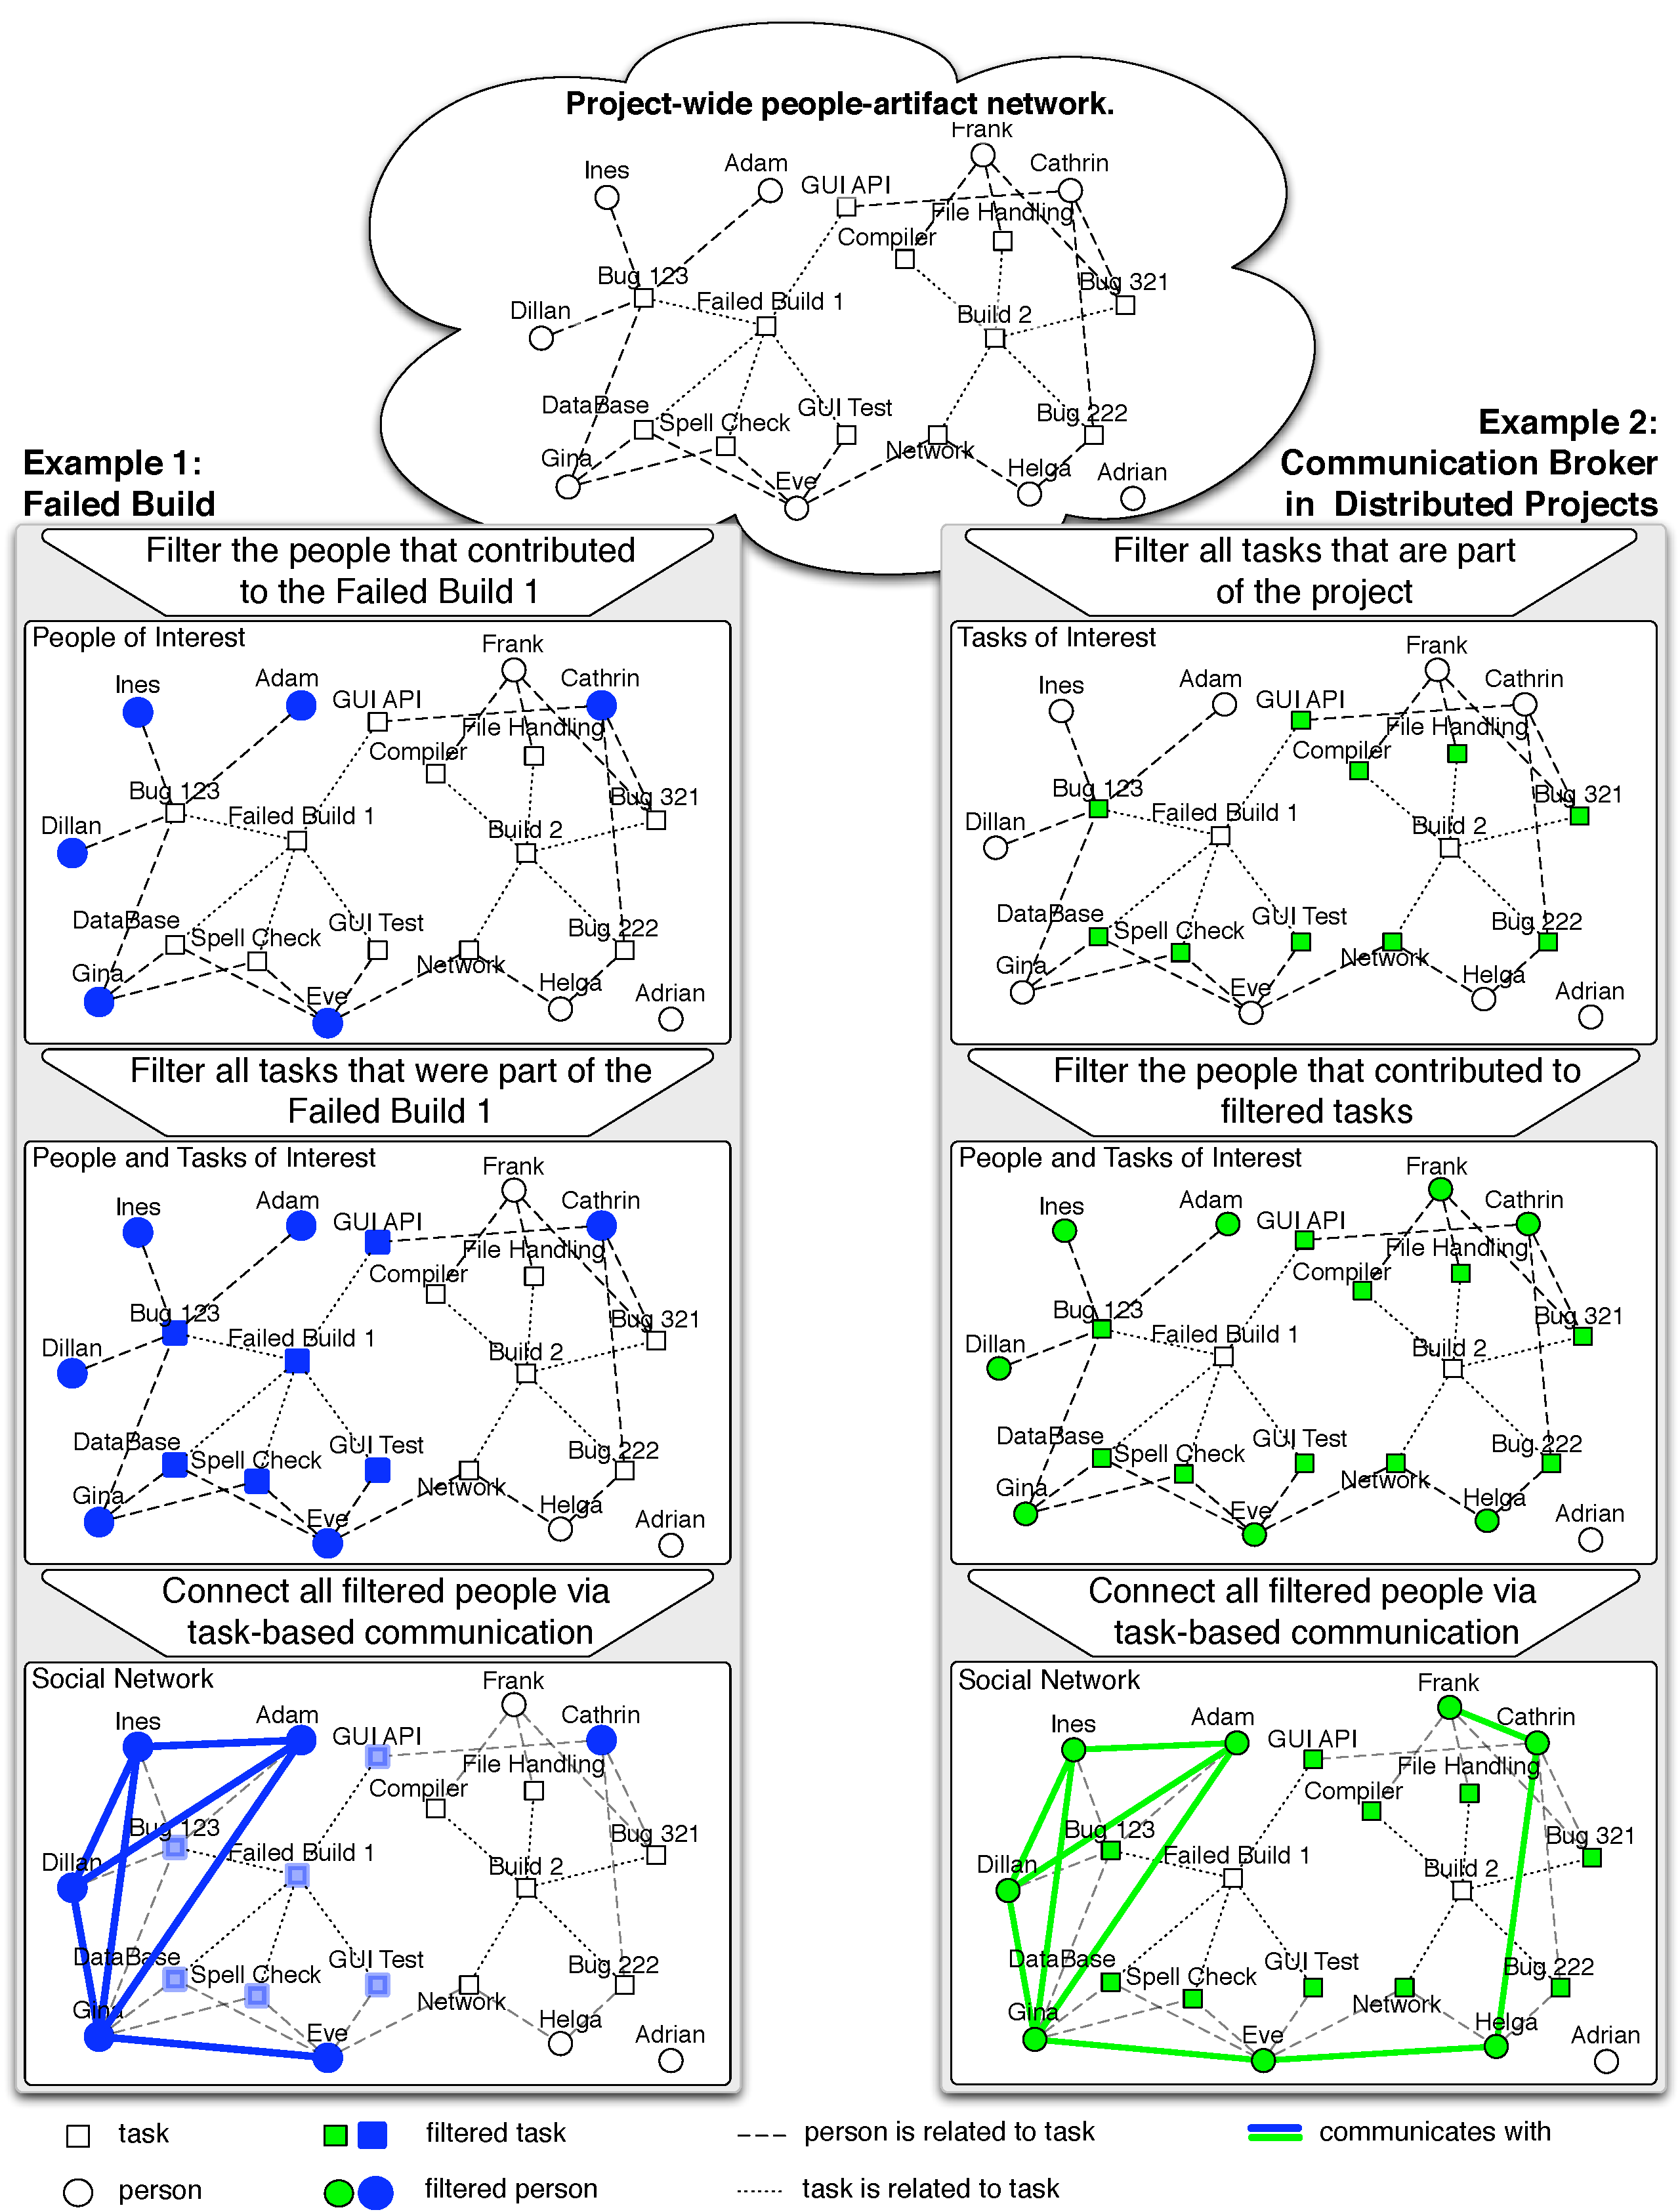
\includegraphics[width=0.8\columnwidth]{./figures/grand_figure}
%\caption{Social network construction examples in our approach}
%\label{fig:network}
%\end{center}
%\end{figure}
A social network is represented as a graph that consist of nodes connected by edges. 
In our approach, the nodes represent people and edges represent task-related communication between these people.

The approach is repository and tool independent and can be applied to any repositories that provide information about people, tasks, technical artifacts, and communication, this includes work, issue, or change management repositories, such as Bugzilla or IBM Rational Team Concert; or source code management systems, such as CVS or IBM Rational Team Concert; or even communication repositories such as email archives.

There are three critical elements that are necessary to construct task-based social networks for a collaboration scope and that need to be mined from software development repositories.
\emph{Project Members}  can be developers, testers, project managers, requirements analysts,
or clients. 
\emph{Work Items} are units of work within the project that may create a need to collaborate and communicate such as a bug report or feature request.
\emph{Work Item Communication} is the information exchanged while completing a work item and is the unique information that allows us to build task-based social networks.


%The data underlying the social network used throughout this thesis are based on work items and their associated discussions.
%In IBM Rational Team Concert each work item has an attached discussion thread were developers can discuss the work item or simply note down their thoughts while working on the work item.
%This means, we would create a link between two developer if they comment together on the same work item to indicate that they are part of the same discussion.
%Note that this sections draws heavily from our work done in collaboration with Timo Wolf, Daniela Damian, Lucas Panjer, and Thanh Nguyen~\cite{wolf:ieee:2009}.

\subsubsection{Technical Network}
%\begin{figure}[th!]
%\centering
%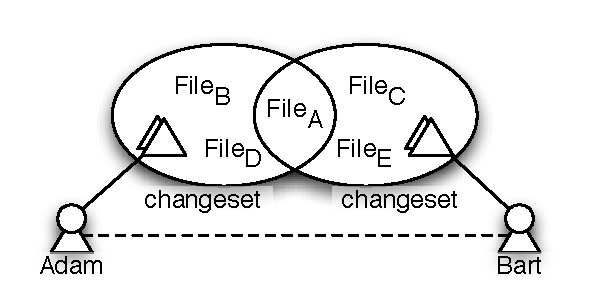
\includegraphics[width=.9\columnwidth]{figures/cochangedfiles}
%\caption{Creating a technical network by connecting developers that changed the same file.}
%\label{fig:construct-tn}
%\end{figure}

% some preamble as in the previous subsection
Building technical networks follows a very similar approach as we described for building social networks.
In fact, the technical network is a social network whose main distinction from the social network described earlier lies in the way edges between nodes are created.
We derive the name of technical network from the way we link developer with each other, namely if they are modifying related source code artifacts.
As in the previous network construction, the construction of the technical network is based on three components.
%
%\begin{itemize}
\emph{Project Members}  can be developers, testers, project managers, requirements analysts,
or clients or in general anyone that modifies software artifacts through change-sets. 
%
\emph{Change-Sets} consist of a number of artifacts that have been modified as well as the modifications themselves.
%
\emph{Software Artifact Relation}  can be defined in several different ways.
For example, in Figure~\ref{fig:construct-tn} Alfred and Bob are related through a technical relationship because they modified the same file.
%\end{itemize}

% Example as shown in the picture
Constructing technical networks therefore follows three steps: (1) we gather all change-sets of interest, (2) identify the relations between artifacts, (3) infer from the change-sets and the relations between the source code artifacts the relation between the artifact owners.
%For example, after we selected the set of change-sets of interest we define the change-sets themselves as the source code artifact and identify the owners of those artifacts.
%Then we infer the relationship between those source code artifacts by relating all change-sets that changes the same source code file.
%And as Figure~\ref{fig:construct-tn} shows this means in the case for Alfred and Bob that they are connected because both own a change-set that modifies the same file.

\subsubsection{Socio-Technical Network}
\begin{figure*}[t!]
%	
  \centering
  \subfloat[Inferring to the build focus relevant change-sets and work items.]{
    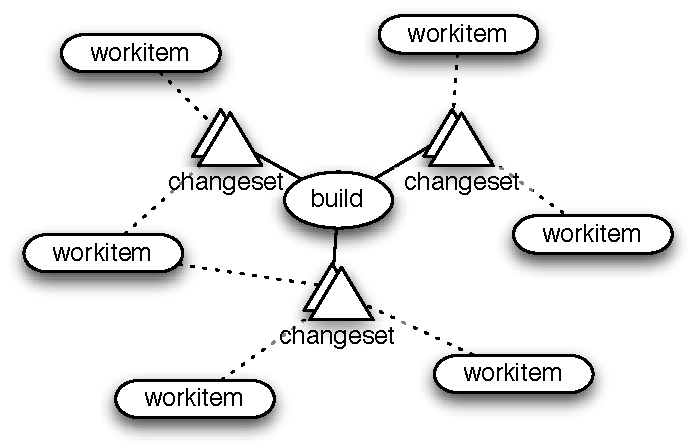
\includegraphics[width=.22\textwidth]{figures/buildworkitem}
    \label{fig:construct-focus}
  }
% 
\hspace{5pt}
  \subfloat[Constructing an social networks from work item communication.]{
	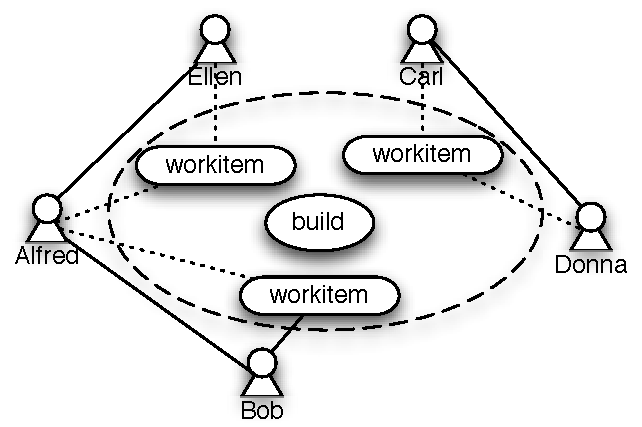
\includegraphics[width=.22\textwidth]{figures/buildsn}
     \label{fig:construct-sn}
  }
\hspace{5pt} 
    \subfloat[Linking developers in a technical networks via change-set overlaps.]{
  	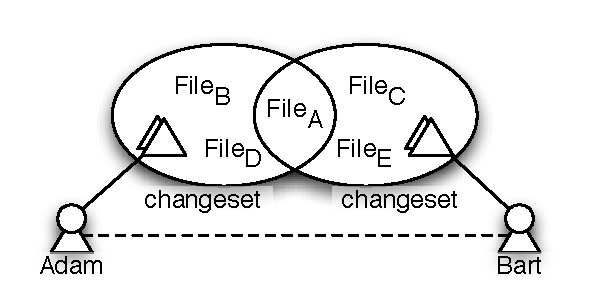
\includegraphics[width=.22\textwidth]{figures/cochangedfiles}
    \label{fig:construct-tn}
  }
\hspace{5pt}
  \subfloat[Combine social and technical networks into a socio-technical network.]{
  	\includegraphics[width=.22\textwidth]{figures/stc-net}
	\label{fig:construct-combine}
  }
  \caption{Constructing socio-technical networks from the repository provided by the IBM Rational Team Concert development team.}
  \label{fig:construct-stc}
\end{figure*}

Socio-Technical networks are a meaningful combination of both social and technical networks.
Selecting this meaningful combination reflects itself in the selection of the work-items in the case of building the social network and selecting the change-sets and their relations in the case of the technical network.
Hence constructing a socio-technical network requires the following four steps:

\begin{enumerate}
\item\textbf{Selecting the Focus} used for the socio-technical network represents the glue that binds the social and technical network into a socio-techncial network. 
This focus also referred to as filter in our earlier publication~\cite{wolf:ieee:2009}, determines the content of the networks.
\item\textbf{Constructing the Social Network} we build social networks from all work items that are relevant to the defined focus.
\item\textbf{Constructing the Technical Network} follows the description of constructing technical networks above with the focus determining the change-sets being used to determine and connect developers in the network.
\item\textbf{Combining Networks} overlays the networks by unifying the set of developers in both networks.
\end{enumerate}

% describe the example in the figure
Figure~\ref{fig:construct-stc} shows an example on how we in our studies of the IBM Rational Team Concert development team used to create socio-technical networks.
In the first step (Figure~\ref{fig:construct-focus}) we set the focus to be a software build which allows us via the change-sets that made it into the build to infer what work items are also represented in said build.
Given the focus, the social network can be constructed using the work items that can be linked to the software build (Figure~\ref{fig:construct-sn}).
Similarly the construction of the technical network relies on the change-sets that went into a build. 
To actually infer edges between developer, we relying on co-changed files within a build as an indicator of work dependency (Figure~\ref{fig:construct-tn}).
Finally, the two networks are combined and yield the socio-technical network shown in Figure~\ref{fig:construct-combine}.

\subsection{Data Collection Methods}
\label{c5:sec:datacollection}
To conduct our research we drew upon multiple data sources.
We employ repository mining techniques to identify larger trends in measurable activities.
In contrast to gain a more in-depth understanding on how developers actually work and deal with interdependencies especially how they would react to certain recommendations and whether they are can be made useful we employ qualitative methods.

\subsubsection{Repository Mining}
Software development usually uses a number of tools to manage information electronically such as version archives and issue trackers.
Additionally to storing source code and tasks/issues, those software repositories can also contain digital communication such as forum and email discussions.

%Repositories can grow to considerable sizes depending on the projects live span and intensity. 
%Therefore, it is often infeasible to manually review the history of a project and it is necessary to employ data-mining techniques to be able to analyze trends.
%Data mining approaches leveraging this wealth of data are one way to easily give back value to the development team without burdening any individual developer with diverting time to other non-automatic data collection instruments.
%technical congruence to generate actionable recommendations.
%In case a developer needs to personally provide a large amount of information manually the overhead generated by a system might outweigh the benefit of recommendations and therefore make the system useless.

We extract information from three different types of repositories: (1) version control, (2) task management, and (3) build engine systems.
The version control supplies us with the knowledge on how developers are connected through their technical work.
The task management supplies us with the information on who communicated with whom with respect to a work item.
And lastly the build engine supplies us with the focus to construct socio-technical networks.

In order to derive socio-technical networks we need to link the different artifact types.
Within IBM Rational Team Concert as illustrated in Figure~\ref{fig:construct-focus} work items are linked to change-sets and change-sets are linked to builds, therefore, establishing the connections needed to construct socio-technical networks with a build as focus.

\subsubsection{Surveys}
To complement the insights we obtained from mining repositories we use surveys.
Surveys are designed iteratively and piloted before deployment, and intended to collect input to enrich and clarify information obtained from the software repositories. 
With each survey we try to minimize the time each developer needs to spend completing them, which usually limits ourselves to focus on closed questions.
We constrain ourselves in this way to minimize the distraction to each individual developer and thus increase the response rate.

Our surveys are deployed through web services to make the collections more convenient to each developer as they are spending most of their times working at a computer enabling them to fill out the survey at their earliest convenience.
Keeping track of a paper version is more cumbersome as they might not easily be returned, especially considering that the development teams we are collaborating with are distributed across different continents.


\subsubsection{Observations}
The next richer and also to the developer more distracting method of data gathering are observations.
Although not necessarily actively interrupting and distracting developer, the act of observing can distract developers and also change their behaviour.
In order to minimize this type of distraction and to mitigate the observer bias, we employed a special form of observation study namely participant observation.
In short we became both an observer and a participant.
%
Being a participant observer has a multitude of advantages:

%\begin{itemize}
\emph{Reciprocity.} By participating in the actual development we can provide value to the development team from the very beginning.
This, in turn, motivates the developers to give us the time we need to conduct other parts of the study, like surveys and interviews.
\emph{Learning the Vocabulary.} Each development project has its own project vocabulary~\cite{espinosa2007:team_knowledge} in order to effectively and clearly communicate. 
Understanding this vocabulary as an outsider is not necessarily easy but very important to make sense of comments and answers supplied in interviews and surveys.
\emph{Understanding the Context.} For example, in one study our observation period coincided with the months prior to a major release. 
% something about the context helping
Because of this closeness of our observation period to a major release we observed mainly activities around integration testing with little coding activity aside from fixing major bugs.

%Although it is easy to ascertain when the next major release of the product is, the effect this has on the developer besides a change in the process is harder to gauge.
%Being part of the development effort allowed us to better understand how developers react to the change in process and better understand their struggles.

\emph{Asking more Meaningful Questions.} A better understanding of the project and how it affects the individual developer as well as understand the vocabulary helps with phrasing better questions.
%Better in the sense of both more meaningful to the developer and in the sense of understandability because they can be phrased using the project vocabulary.
%\end{itemize}

Besides gaining a better understanding of some easily missed or miss-understood intricacies, working together with the developer establishes a trust relationship~\cite{letherbridge:ese2005}.
This trust helps to mitigate observation biases that are introduced by just observing as well as makes developers more forthcoming during interviews and surveys~\cite{letherbridge:ese2005}.
%We were able to join the Rational Team Concert development team as a participant observer mainly due to the convincing argument that we take the place of an intern, thus, contributing to their development effort (Chapter~\ref{chap:talk})

\subsubsection{Interviews}
To further enhance our understanding on how developers view the situation, we employed interviews.
Instead of following a structured interview approach, we opt for a semi-structured interview with a focus on war stories.
War stories~\cite{lutters:ist:2007} ask the interviewee to share memorable stories from work life.
The interviewer than can explore those war stories and help shape the focus of the discussion of those events.
This type of interview comes with two major benefits over structured interviews that follow a set of questions:

%\begin{itemize}
\emph{Focus onto for the interviewee important events.}
Knowing the pain points as they are perceived by the projects participants allows us to focus on important issues.
With prepared questions the focus of the interview might not uncover what is important to the interviewee and thus we might miss areas.
\emph{Better recall of events by interviewee.}
Recall of events of importance is better than of arbitrary events~\cite{lutters:ist:2007}.
This allows us to place more confidence into the reports and answers given by the interviewees.
%\end{itemize}

%The main drawback of using war stories over prepared interview questions in a structured interview framework lies with the loss of focus of the interviews.
By asking the interviewee to tell war stories of memorable events it can be more difficult to gain the insights into a particular area of interest if the war stories veer to far off the topic of interest.
It is therefore necessary that the interviewer has a good understanding of the project and the project language to explore the stories for relevance to topics of interest making it thus more demanding on the side of the interviewer.

% talk about the time of the interviews
%We tried to minimize the interruption to project members as much as possible therefore we limited the time we require for each interview as much as possible.
%Most interviews are aimed at taking 30 minutes with a 30 minute overflow in case a participant is willing to continue the interview.
%Furthermore, we gave the work of the interviewee priority over the interview and assured the interviewees that they could stop the interview anytime they felt that their work needs attention.
%This was especially valuable with a professional development team such as the IBM Rational Team Concert development team as we joined their development effort when they were nearing a major milestone (Chapter~\ref{chap:talk}).












% !TEX root = thesis-journal.tex
\section{Communication and Failure}
\label{chap:soc-net}
We open our investigation of how to modify the social relationships among software developers, represented by the communication between them, with searching for a relationship between communication and build success.
This forms the basis and justification for an approach that we describe in a later chapter to allow us to manipulate the social interactions among developers.
Thus this chapter explores our first research question:
\begin{description}
\item[RQ 1.1] Do Social Networks influence build success?
\end{description}

A connection between communication among developers and any sort of software quality including software builds makes intuitively sense.
For example, any non trivial software project consists of several interdependent modules and with the growing size and number of modules the work of more than one software developer is required to finish the project within a certain time constraint often mandated by a customer.
Now due to the interdependence of the software modules developers assigned either to the same or to interdependent modules need to coordinate their work.
This coordination is in the most part accomplished through communication, which can take any form from a face-to-face discussion to electronically asynchronous messages such as email.
Coupled with the fact that communication is inherently ambiguous and can often lead to misunderstandings, errors based on such misunderstandings may be introduces into the source code.
Thus, we are confident that there exists  a connection between developer communication and build success.

In this chapter, we start with describing the methodology that is relevant to exploring our research question (Section~\ref{sec:Methodology}).
Then, we present our analysis and results we obtained in Section~\ref{sec:AnalysisResults} followed by a discussion of the results in Section~\ref{sec:discussion}.
We conclude this chapter with offering an answer to our research question and leading into the subsequent Chapter~\ref{chap:stc-net2} (Section~\ref{sec:conclusion}).


\subsection{Methodology}
\label{sec:Methodology}
To address our research question we analyze data from a large software
development project IBM Rational Team Concert which we described in created detail in Chapter~\ref{chap:rtc}.

\subsubsection{Coordination outcome measure}
In our study we conceptualize the coordination outcome by the Build Result,
which is regarded as a coordination success indicator in Jazz and can be \error,
\texttt{WARNING} or \ok. We analyze build results to examine the integration
outcomes in relation to the communication necessary for the coordination of the
build.

Conceptually, the \texttt{WARNING} and \ok\ build results are treated similar by
the Jazz team, as they require no further attention or reaction from the
developers. In contrast, \error\ build results indicate serious problems such as
compile errors or test failures and require further coordination, communication
and development effort. We thus treated all \texttt{WARNING}s as \ok s to clearly
separate between failed and successful builds in our conceptualization of
coordination outcome.


\subsubsection{Communication network measures}
To characterize the communication structure represented by the constructed social
networks for each build (as described in Chapter~\ref{chap:meth}), we compute a number of social network measures. The
measures that we include in our analysis are: Density, Centrality and Structural
holes. Some of these measures characterize single nodes and their neighbours (ego
networks), while others relate to complete networks. As we are interested in
analysing the characteristics of complete communication networks associated to
integration builds, we normalize and use appropriate formulas to measure the
complete communication networks instead of measuring the individual nodes.

\paragraph{Density}
Density is calculated as the percentage of the existing connections to all
possible connections in the network. A fully connected network has a density of
1, while a network without any connections has the density of 0. For example, the
density in the directed network in Figure~\ref{fig:CentralityExample} is
$12/42=0.28$.

\paragraph{Centrality measures}
We use the centrality measures \emph{group degree centralization} and
\emph{group betweenness centralization} for complete networks, which are based on
the ego network measures degree centrality and betweenness. The degree
centrality measures for the ego networks are:

\begin{itemize}
  \item The \emph{Out-Degree} of a node $c$ is the
  number of its outgoing connections $C_{oD}(c)$. E.g. $C_{oD}(c_1)=2$ in 
  Figure~\ref{fig:CentralityExample}.
  
  \item The \emph{In-Degree} of a node $c$ is the
  number of it s incoming connections $C_{iD}(c)$. For example $C_{iD}(c_1)=1$ 
  in Figure~\ref{fig:CentralityExample}.
  
  \item The \emph{InOut-Degree} of a node $c$ is the sum of its In-Degree and
  Out-Degree $C_{ioD}(c)$. E.g. $C_{ioD}(c_1)=3$
  in Figure~\ref{fig:CentralityExample}.
\end{itemize}

To compute the \emph{Group Degree Centralization} index for the complete network
we use formula~(\ref{eq:GroupDegreeCentralization}) from
Freeman~\cite{Freeman:1979rl}, in which $g$ is the number of nodes in a network,
and $C_D(c_i)$ is any of the degree centrality measures of a node $c_i$ as
described above. $C_D(c^*)$ is the largest node degree index for the set of
contributors in the network. The formula is also used
by~\cite{Gloor:2003cikm,hinds:cscw:2006}.

\begin{equation}
\displaystyle C_D =  \frac{\sum_{i=1}^g[C_D(c^*) - C_D(c_i)]}{(g-1)^2}
\label{eq:GroupDegreeCentralization}
\end{equation}

\begin{figure}[t]
\begin{center}
\includegraphics[width=.8\columnwidth]{figures/CentralityExample}
\caption{Example of a directed network to illustrate our social
analysis measures.}
\label{fig:CentralityExample}
\end{center}
\end{figure}

To calculate the \emph{Group Betweenness Centralization} index for a whole
network, we need to compute the betweenness centrality probability index for each
actor of the network. The probability index assumes that a ``communication''
takes the shortest path from a contributor $c_j$ to contributor $c_k$ and if the
network has more shortest paths, all of them have the same probability to be
chosen. If $g_{jk}$ is the number of shortest paths linking two contributors,
$1/g_{jk}$ is the probability of using one of the shortest paths for
communication. Let $g_{jk}(c_i)$ be the number of shortest paths linking two
contributors that contain the contributors $c_i$. Freeman~\cite{Freeman:1979rl}
estimates the probability that contributor $c_i$ is between $c_j$ and $c_k$ by
$g_{jk}(c_1)/g_{jk}$. The betweenness index for $c_i$ is the sum of all
probabilities over all pairs of actors excluding the $i$th contributor.
Formula~(\ref{eq:Betweenness}) shows the normalized betweenness index for
directed networks.

\begin{equation}
\displaystyle C_B(c_i) =  \frac{\sum_{j<k} g_{jk}(c_i)/g_{jk}}{(g-1)(g-2)}
\label{eq:Betweenness}
\end{equation}

To compute a betweenness index for the complete network instead of a single node,
we used Freeman's formula for \emph{Group Betweenness Centralization}. The
formula is shown in equation~(\ref{eq:GroupBetweenness}), in which $C_B(c^*)$ is
the largest betweenness index of all actors in the network.

\begin{equation}
\displaystyle C_B =  \frac{\sum_{i=1}^g[C_B(c^*)-C_B(c_i)]}{(g-1)}
\label{eq:GroupBetweenness}
\end{equation}


\paragraph{Structural holes}
We use the following structural hole measures:
\begin{itemize}
  \item The \emph{Effective Size} of a node $c_i$ is the number of its
  neighbours minus the average degree of those in $c_i$'s ego network, not
  counting their connections to $c_i$. The effective size of node $c_1$ in 
  Figure~\ref{fig:CentralityExample}a is $2-1=1$. Note, that only direct
  neighbours of $c_1$ are considered and the directed connections are replace
  with undirected. The effective size of node $c_4$ in 
  Figure~\ref{fig:CentralityExample}b is $2-0=2$.
  
  \item The \emph{Efficiency} normalizes the effective size of a node $c_i$ by
  dividing the it's effective size with the number of it's neighbours. The
  efficiency of node $c_1$ in Figure~\ref{fig:CentralityExample}a is
  $(2-1)/2=0.5$. The efficiency of node $c_4$ in
  Figure~\ref{fig:CentralityExample}b is $(2-0)/2=1$.
  
  \item \emph{Constraint} is a summary measure that relates the connections of a
  node $c_i$ to the connections of $c_i$'s neighbours. If $c_i$'s neighbours and
  potential communication partners all have one another as potential communication
  partners, $c_i$ is highly constrained. If $c_i$'s neighbours do not have other
  alternatives in the neighborhood, they cannot constrain $c_i$'s behavior. 
\end{itemize}

To calculate network measures of the introduced ego network measures on
structural holes, we compute the sum of the measures for each node of a network.
As the measures are based on network connections, we normalize the sum by
computing the fraction of the sum and the number of possible network connections.

\subsubsection{Data collection} 
We mined the Jazz development repository for build and communication information.
A query plug-in was implemented to extract all development and communication
artifacts involved in each build from the Jazz server. These build-related
artifacts included build results, teams, change sets, work items, contributors,
and comments. We imported the resulting data into a relational database
management system to handle the data more efficiently.

We extracted a total of 1288 build results, 13020 change sets, 25713 work items
and 71019 comments. Out of a total of 47 Jazz teams, 24 had integration builds.
The build results we extracted were created during the time range from
November~5, 2007 to February~26, 2008.

Next, we had to make a decision which builds and associated communication to
analyze. Our selection criteria was that we analyze a number of build results
that is large enough for statistical tests and include both \ok\ and \error\
builds. Some teams used the building process for testing purposes only and created
just a view build results, while others had either only \ok\ or only \error\
build results. Predicting build results for a team that only produced \error\
builds in the past, will most likely yield an \error, since no communication
information representing successful builds is available. Thus, we considered
teams that had more than 30 build results and at least 10 failed and 10
successful builds. Five teams satisfied these constraints and were considered in
our analysis. In addition, we included the nightly, weekly, and one beta
integration build, although they did not satisfy our constraints, because 
they integrate all subsystems of the entire project.






\subsection{Analysis and Results}
\label{sec:AnalysisResults}
Table~\ref{tab:DescriptiveStats} shows descriptive statistics of the considered
builds and related communication networks of the five teams (B, C, F, P and W in
the first 5 columns) and the nightly, weekly, and beta project-level
integrations. For example, team B created 60 builds from which 20 turned out to
be \error s and 40 \ok. The communication networks of this team had between 3 and
58 contributors (51.58 directed connections in average) and spanned 0 to 131 work
items. The builds involved in average 10.83 change sets.

\begin{table}[t]
\footnotesize
\begin{center}
%{\small
\begin{tabular}{r@{\hspace{9pt}}c@{\hspace{4pt}}c@{\hspace{4pt}}c@{\hspace{4pt}}c@{\hspace{4pt}}c@{\hspace{9pt}}c@{\hspace{4pt}}c@{\hspace{4pt}}c}
\toprule
%  & & & Teams & & & & & &  \\
& \multicolumn{5}{ c@{\hspace{3pt}}}{Team Level Builds} &
\multicolumn{3}{c}{Project Level Builds} \\ & B & C & F & P & W & nightly &
weekly & beta
\\
\midrule
\# Builds & 60 & 48 & 55 & 59 & 55 & 15 & 15 & 16 \\ 
\# \error s & 20 & 16 & 24 & 29 & 31 & 9 & 11 & 13 \\ 
\# \ok s & 40 & 32 & 31 & 30 & 24 & 6 & 4 & 3 \\ 
%First Build & 2007-11-05 14:04:48 & 2007-11-09 07:22:05 & 2007-11-06 03:36:48
%& 2007-11-05 22:28:45 & 2007-11-09 17:01:35 & 2007-11-05 03:59:06 & 2007-07-24
%21:19:07 & 2007-12-04 14:23:20 \\ 
%Last Build & 2008-02-26 15:43:59 &
%2008-02-26 13:38:49 & 2008-02-22 16:34:25 & 2008-02-26 11:43:36 & 2008-02-26
%08:53:04 & 2008-01-18 07:41:26 & 2008-02-22 15:29:39 & 2008-01-23 19:22:41 \\
\midrule
\multicolumn{3}{l}{\emph{\# Contributors:}} \\
%\midrule
Min & 3 & 9 & 6 & 5 & 13 & 43 & 37 & 55 \\ 
Median & 6 & 16.5 & 18 & 15 & 20 & 55 & 57 & 69.5 \\ 
Mean & 12.68 & 18.02 & 20.15 & 17.98 & 22.87 & 57.93 & 52.27 & 67.81 \\ 
Max & 58 & 31 & 64 & 61 & 52 & 75 & 75 & 79 \\ 
\midrule
%\emph{Connections:}\\ 
\multicolumn{3}{l}{\emph{\# Directed Connections:}} \\
%\midrule
Min & 0 & 1 & 2 & 0 & 11 & 81 & 56 & 144 \\ 
Median & 13 & 39.5 & 95 & 36 & 74 & 236 & 149 & 280 \\ 
Mean & 51.58 & 53.4 & 87.78 & 63 & 88.35 & 253.1 & 171.9 & 285.8 \\ 
Max & 361 & 139 & 355 & 401 & 300 & 434 & 496 & 446 \\ 
\midrule
%\emph{Change Sets:}\\ 
\multicolumn{3}{l}{\emph{\# Change Sets:}} \\
%\midrule
Min & 1 & 15 & 8 & 32 & 83 & 80 & 62 & 82 \\ 
Median & 10 & 38 & 35 & 46 & 111 & 117 & 115 & 178.5 \\ 
Mean & 10.83 & 44.38 & 42.65 & 47.25 & 115.3 & 129 & 114.2 & 166.8 \\ 
Max & 33 & 101 & 91 & 75 & 156 & 199 & 173 & 196 \\ 
\midrule
%\emph{Work Items:}\\
\multicolumn{3}{l}{\emph{\# Work Items:}} \\
%\midrule 
Min & 0 & 2 & 1 & 1 & 10 & 11 & 5 & 31 \\ 
Median & 6.5 & 12 & 20 & 12 & 18 & 67 & 51 & 98 \\ 
Mean & 16.43 & 15.56 & 23.07 & 19.34 & 29.49 & 72.13 & 56.87 & 96.81 \\ 
Max & 131 & 50 & 100 & 107 & 119 & 132 & 202 & 170 \\ 
\bottomrule
\end{tabular}
\end{center}
\caption{Descriptive build statistics.}
\label{tab:DescriptiveStats}
\end{table}

\subsubsection{Individual communication measures and build results}
To examine whether any individual measure of communication structure can predict
integration failure or success, we analyze the builds
from each team and project-level integration in part in relation to the
communication structure measures as follows: For each team we categorize the
builds into two groups. One group contains the \error\ builds and the other the
\ok\ builds. For each build and associated communication network we compute the
network measures described in Section~\ref{sec:Methodology} and compare them
across the two groups of builds (\error\ and \ok).

The communication measures used in the analysis were: Density, Centrality
(in-degree, out-degree, inout-degree, and betweenness), Structural Holes
(efficiency, effective size, and constraint), and number of directed connections.
We used the Mann-Whitney test~\cite{Siegel:1956tu} to test if any of the measures
differentiate between the groups of \error\ and \ok\ related communication
networks. We used the $\alpha$-level of $.05$ and applied the Bonferroni
correction to mitigate the threat of multiple hypothesis testing. None of the
tests yielded statistical significance, which indicates that no individual
communication structure measures significantly differentiate between \error\ and
\ok\ builds.

We also tested for the possible effect of the technical measures shown in
Table~\ref{tab:DescriptiveStats}: \#Contributors, \#Change Sets and the \#Work
Items on the build result. Also, none of the tests yielded statistical
significance to differentiate between \error\ and \ok\ builds.


\subsubsection{Predictive power of measures of communication structures}

We combined communication structure measures into a predictive model
that classifies a team's communication structure as leading to an \error\ or \ok\
build. We explicitly exclude the technical descriptive measures such as
\#Contributors, \#Change Sets and the \#Work Items from the model in order to
focus on the effect of communication on build failure prediction. We validate the
model for each set of team-level and project-level networks separately by
training a Bayesian classifier~\cite{Hastie:2003ys} and using the leave one
out cross validation method~\cite{Hastie:2003ys}.

For example, to predict the build result N of team F's 55 build results, we train
a Bayesian classifier with all other 54 build results and their communication
related network measures. Then, we input the communication measures of Build N's
related communication network into the classifier and predict the result of build
N. We repeat the classification for all 55 builds of team F and sum up the number
of correctly and wrongly classified results.

\begin{table}[t] \centering\small
\begin{tabular}{lc}
& prediction \\
actual & 
\begin{tabular}{r|c|c|}
& \ok\ & \error\ \\\hline
\ok\ & 26 & 5 \\\hline
\error\ & 9 & 15 \\\hline
\end{tabular}
\end{tabular}
\caption{Classification results for team F.}
% \caption{Classification results for continuous build definition of team F, 26
% builds were correct as \ok\ and 5 wrong as \error\ classified.}
\label{tab:cont}
\end{table}

Table~\ref{tab:cont} shows the classification result for team F. The upper left
cell represents the number of correctly classified communication networks as
related to \ok\ builds (26 vs. 31 actual), and the lower right cell shows the
number of correctly classified networks as leading to \error\ builds (15 vs. 24
actual). The other two cells show the number of wrongly classified communication
networks.

The classification quality is assessed via recall and precision coefficients,
which can be calculated for \error\ and \ok\ build  predictions. We explain the
coefficients for prediction of \error\ builds.
% same definition as Tom's paper need to look up gail's definition

\begin{itemize}
\item\textbf{Recall} is the percentage of correctly classified networks as leading to
\error\ divided by the number of \error\ related networks. In
Table~\ref{tab:cont} the lower right cell shows the number of correct classified
networks that are leading to \error s, which is divided by the sum of the values
in the lower row, which represents the total number of actual \error s. This
yields for Table~\ref{tab:cont} a recall of $15/(9+15)=.62$. In other words,
62\% of the actual to \error\ leading networks are correctly classified.
 
\item\textbf{Precision} is the percentage of as to \error\ leading classified networks
that turned out to be actually \error s. In Table~\ref{tab:cont}, it is the
number of correctly classified \error s divided by the sum of the right column,
which represents the number of as \error\ classified builds. In
Table~\ref{tab:cont} the precision is $15/(5+15)=.75$. In practical terms, 75\%
of the \error\ predictions are actual \error s.
\end{itemize}


\begin{table}[t] \small
\begin{center}
%{\small
\begin{tabular}{ r@{\hspace{10pt}}c@{\hspace{4pt}}c@{\hspace{4pt}}c@{\hspace{4pt}}c@{\hspace{4pt}}c@{\hspace{10pt}}c@{\hspace{4pt}}c@{\hspace{4pt}}c}
\toprule
& \multicolumn{5}{c}{\hspace{-15pt}Team Level Builds} &
\multicolumn{3}{c}{Project Level Builds} \\
%\textbf{Naive Bayes} & & & & & & & \\
& B & C & F & P & W & nightly & weekly & beta 	 \\
\midrule
\error\ Recall & .55 & .75 & .62 & .66 & .74 & .89 & 1 & .92 \\ 
\error\ Precision & .52 & .50 & .75 & .76 & .66 & .73 & .92 & .92 \\ 
\ok\ Recall & .75 & .62 & .84 & .80 & .50 & .50 & .75 & .67 \\ 
\ok\ Precision & .77 & .83 & .74 & .71 & .60 & .75 & 1 & .67 \\ 
\bottomrule
\end{tabular}
\end{center}
\caption{Recall and precision for failed (\error) and successful (\ok) build results using
the Bayesian classifier.}
\label{tab:PredictionResultTable}
\end{table}


We repeated the classification described above for each team and project-level
integration. Note that the model prediction results only show how the models
perform within a team and not across teams. Table~\ref{tab:PredictionResultTable}
shows the recall and precision values for as to \ok\ and \error\ leading
classified communication networks for each of the five team-level and three
project-level integrations. Since we are interested in the power of build failure
prediction, the error related values from our model are of greater importance to
us. The \error\ recall values (how many \error s were classified correctly) of
team-level builds are between 55\% and 75\% and the recall values of the
project-level builds are even higher with at least 89\%. The \error\ precision
values are equally high.






\subsection{Discussion}
\label{sec:discussion}
In our analysis we examined the relationship between integration builds and
measures of the related communication structure. We found that none of the single
communication structure measures (density, centrality or structure hole measures)
significantly differentiated between failed and successful builds at the
team-level and project-level. Therefore none of these individual communication
structure measures could be used to predict integration build results.

In addition to the communication related measures, we also examined whether the
technical measures we computed when constructing the communication networks --
the number of change sets, contributors, and work items -- have an impact on the
integration build result, as they are an indication for the size and complexity
of the development tasks to be coordinated. According to Nagappan and
Ball~\cite{nagappan:icse:2005}, one might expect that increased size and complexity
of code changes relates to more build failures. But in our study these single
measures did not significantly differentiate between successful and failed build
results. However, additional technical measures that were used by Nagappan might
be good predictors in Jazz as well.

The second contribution of this work is the predictive model that uses measures
of communication structures to predict build results. Interestingly, the
combination of communication structure measures was a good predictor of failure
even when the single measurements were not. Our model's precision in predicting
failed builds, which relates to the confidence one can have in the predicted
result, ranges from 50\% to 76\% for any of the five team-level integration
builds, and is above 73\% for the project-level integration builds.

We found that, for all prediction models, the recall and precision values are
better than guessing. A guess is deciding on the probability of an \error\ or an
\ok\ build if the build fails or succeeds. The probability is the number of
\error s or \ok s divided by the number of all builds. For example, if we know
that the \error\ probability is 50\% and we guess the result of the next build we
would achieve a recall and precision of 50\%. In our case, our model reached an
\error\ recall of 62\% for team F, where as a guess would have yield only
$24/55=.44=$ 44\% (see Table~\ref{tab:DescriptiveStats}).

\subsection{Conclusions}
\label{sec:conclusion}
We conclude this chapter by bringing it back to the initial research question we set out to answer:
\begin{itemize}
\item\textbf{RQ 1.1} Do Social Networks from repositories influence build success?
\end{itemize}

The result we presented in Section~\ref{sec:AnalysisResults} show that our predictions, though not highly accurate, outperform random guesses.
Therefore, we conclude that with recall of 55\% to 75\% and precision of 50\% to 76\%, depending on the development team, that communication indeed influences build success.

This finding opens the research avenue of investigating whether the manipulation of communication among software developers can yield positive results with respect to build success.
This leads us to the next research question that we want to search for places within the social networks that we should manipulate to stimulate build success.
For that purpose we turn in the next chapter to the concept of socio-technical congruence that might help us highlighting those developers that should have communicated.



% !TEX root = thesis-journal.tex
\section{Socio-Technical Congruence and Failure}
\label{chap:stc-net2}
Knowing that social networks have an effect on build success opens the next question as to how or more precisely which parts of the social network should be changed to increase the likelihood for a build to succeed.
For this reason we turn to the concept of socio-technical congruence as it postulates that developers should communicate once their work intersects.
Thus in this section we explore the effect of socio-technical networks on build success:

\begin{itemize}
  \item\textbf{RQ 1.2:} Does Socio-Technical Networks influence build success?
\end{itemize}

Although socio-technical congruence has only been studied in connection with productivity intuitively there should be a connection to software quality such as build success.
For example, imagine two developer modifying classes that share call and data dependencies and one developer making changes that violate certain assumptions the other developer relies on when using the modified code.
This might introduce an error that could have been prevented if both developer would have discussed their work.
Thus, we hypothesize that the concept of socio-technical congruence relates to software quality as well as productivity and might be used to point developers towards improvements in the social network by pointing out developers that should communicate.




\begin{table}[t]
\begin{center}
%\small
\begin{tabular}{l@{\hspace{0pt}}r@{\hspace{10pt}}r@{\hspace{5pt}}r}
\toprule
Variable & Coef. & S.E. & \emph{p} \\
	\midrule
Intercept                   &  -0.5459 &   0.4663 & 0.2417 \\
\textbf{Congruence}              &   \textbf{6.3410} &   \textbf{1.6262} & \textbf{**0.0001} \\
\textbf{Authors}                     &  \textbf{-1.9759} &   \textbf{0.5310} & \textbf{**0.0002}  \\
\textbf{Files}                       &  \textbf{-1.0734} &   \textbf{0.4561} & \textbf{*0.0186}  \\
Work~items                   &  -0.1456 &   0.2355 & 0.5363  \\
\textbf{Build type=I}                      &   \textbf{2.1533} &   \textbf{1.0526} & \textbf{*0.0408}  \\
Build type=N                      &   4.6833 & 200.7587 & 0.9814  \\
Build date                   &  -0.6560 &   0.6709 & 0.3282  \\
\textbf{Congruence * Build type=I}     &  \textbf{-9.2151} &   \textbf{2.5572} & \textbf{**0.0003}  \\
Congruence * Build type=N     &  -7.7308 &  91.8053 & 0.9329  \\
\textbf{Congruence * Build date}  &  \textbf{-5.1266} &   \textbf{1.9290} & \textbf{**0.0079}  \\
Authors $\cdot$ Build type=I            &   1.2688 &   0.7028 & 0.0710  \\
Authors * Build type=N            & 105.4123 & 535.8792 & 0.8441  \\
Authors * Build date         &  -0.6061 &   0.3616 & 0.0937 \\
Authors * Files             &   0.7663 &   0.4289 & 0.0740  \\
Files * Build type=I              &   1.0920 &   1.1838 & 0.3563  \\
Files * Build type=N              & -37.9274 & 199.2314 & 0.8490  \\
\textbf{Work~items * Build date}       &   \textbf{0.8040} &   \textbf{0.3003} & \textbf{**0.0074}  \\
\textbf{Build type=I * Build date}          &   \textbf{2.6442} &   \textbf{0.7678} & \textbf{*0.0006} \\
Build type=N * Build date          &  84.7252 & 344.8129 & 0.8059  \\
	\bottomrule
Model likelihood ratio & 101.92 &  & $R^2=0.581$  \\
\multicolumn{1}{l}{\scriptsize{*$p < 0.05$; **$p < 0.01$}}& \multicolumn{3}{c}{\hspace{-5pt}191 observations}  \\
%\multicolumn{1}{l}{ } & \multicolumn{3}{l}{\tiny{Build type is set to continuous}} \\
%\multicolumn{1}{l}{\scriptsize{*$p < 0.05$; **$p < 0.01$}} & \multicolumn{3}{l}{\tiny{Nagelkerke is used as the pseudo-$R^2$ measure}}
\end{tabular}
\end{center}
\caption{Logistic Regression models predicting build success probability with main and interaction effects}
\label{tab:logr}
\end{table}

\subsection{Calculating Congruence}
\label{sec:congruence}
In Chapter~\ref{chap:meth} we described socio-technical networks and how we conceptualize them in this thesis.
If we reformulate this network into the terms originally used by Cataldo et al~\cite{cataldo:cscw:2006} the matrix representation of the technical dependencies among software developers turns into the coordination needs matrix $CN$ and the social network in matrix representation is the actual coordination matrix $AC$.
Thus we calculate the socio-technical congruence index by deciding the cardinality of $AC$ without $CN$ by the cardinality of  $CN$.



\subsection{Analysis Methods}
\label{sec:methodology}
Logistic regression is ideal to test the relationship between multiple variables and a binary outcome, which in our study is a build result being either ``OK'' or ``Error''. The presence of many data entities in this project means that we must consider confounding variables in addition to the socio-technical congruence when determining its effects on the probability of build success. Informally, logistic regression identifies the amount of ``influence'' that a variable has in the probability that a build will be successful.
The two main variables we are interested in are as aforementioned the socio-techincal congruence index as well as the ratio between gaps and coordination needs, that is technical dependencies among developers that are not accompanies by a corresponding social dependency.


\subsection{Results}
\label{sec:results}
In the RTC repository, we analyzed 191 builds; of these builds, 60 were error builds, and 131 were OK builds.
The congruence values are low on average with a mean value of 0.331 meaning that about one-third of the coordination needs are satisfied by actual coordination.

To assess the fit of the logistic regression models, we use the Nagelkerke pseudo-$R^2$ and AIC. $R^2$ shows the proportion of variability explained by the model, and AIC is a measure of how well the model fits the data. Ideally, $R^2$ is high and AIC is low. Our current model contains 19 variables and has an $R^2$ of 0.581. 
We found that 19 variables is optimal and that removing further variables lowered the $R^2$ value while raising the AIC.


\begin{table}[t]
\begin{center}
\begin{tabular}{lrr}
  \toprule
 & Model\\ 
  \midrule
Intercept & 1.32 \\ 
  Authors &  0.60 \\ 
  Files &  0.63 \\ 
  Work~items  & 0.85 \\ 
  Build type=I  & 1.31 \\ 
  Gap ratio  & 8.71 \\ 
  Build date  & 0.59 \\ 
  Authors * Build date & 0.74 \\ 
  Work~items * Build date  & 1.83 \\ 
  Build type=I * Build date  & 2.52 \\ 
   \bottomrule
\end{tabular}
\caption{Odds Ratio for Gap Ratio Models}
\label{tab:oddsratio_gapsize}
\end{center}
\end{table}

\subsubsection{Effects of interactions involving congruence}
\label{sec:congruenceinteractions}
The type~$\times$~congruence interaction effect, the date~$\times$~congruence interaction, and the type $\times$ date effect are each significant in our model (Table \ref{tab:logr}). 
%
The congruence model (Table \ref{tab:logr}) the effect of congruence on continuous builds is significant, and that increasing congruence also increases the probability that a continuous build will succeed. 
%For integration builds (Figures \ref{fig:unweighted_congruence_typeci_age}, in black), an increase in congruence decreases build success, with the exception of the 2008-01-25 build (Figure \ref{subfig:prob_unweighted_age_typeci_q010}). 
%In in our 2008-01-25 build, we see that low congruence leads to low build probability, but high congruence has high build probability. As the project ages, this trend reverses and congruence is clearly inversely related with build success probability (Figure \ref{subfig:prob_unweighted_age_typeci_q100}).
%The effect of congruence is totally opposite for continuous builds and integration builds. Based on Figure \ref{subfig:prob_unweighted_age_typeci_q100}, increasing congruence significantly improves the continuous build success rate. However, increasing congruence significantly decreases the integration build success rate.


%\subsubsection{Effect of Gap Ratio on Build Result}
%\label{sec:gapsizeresult}
%We build a logistic regression model based on the model in Table \ref{tab:logr} using the gap ratio measurement (percentage of unmet coordination needs). In the interest of saving space, we report only the odds ratio. We retain every significant interaction from our previous congruence logistic regression in Table \ref{tab:logr}.
%
%The effect of gap ratio on build result is significant (see Table~\ref{tab:oddsratio_gapsize}). This indicates that increasing the gaps ratio significantly increases the odds that an OK build will occur, which is the opposite of what we hypothesized. This means that if the gap is large, the build success probability increases.




\subsubsection{Social and Technical Factors in RTC Affecting Build Success and Congruence}
\label{sec:otherfactors}
In light of our results, we examine not only the number of work~items~$\times$~date significant interaction, but different social and technical factors that may affect congruence
and build success probability to find explanations for the interactions between socio-technical congruence and build success probability in RTC.
Specifically, we examine the effect of build date on work items, coordination around fully-congruent builds and
incongruent builds, and the effects of commenting behaviour on builds.




% !TEX root = thesis-journal.tex
\section{The Approach}
\label{chap:approach}
%\section{Formulating the Approach}
Motivated by research showing that socio-technical gaps represetend by low socio-technical congruence (presented in Section~\ref{chap:stc-net2}) increases the chance of a build to fail we formulate an approach that generates actionable knowledge to alleviate socio-technical gaps.
Our approach takes into account the past history of a project analyzing socio-technical gaps with respect to their individual relation to build failure.
These recommendations aim at initiating coordination between two developers that form a gap in the current build, thus increasing the chance of a build to succeed.
This approach can support projects that use electronic repositories such as automated build engines, version control and task management.

For our approach we define a socio-technical gap as the relationship between two developers that share a technical dependency (implying coordination need) without any social interaction (implying unmet coordination need).
A technical dependency can be inferred by two developers changing the same file, or a developer changing a method that another developer's code is calling.
%In this paper, two developers that share a technical dependency are referred to as a \emph{technical pair} (or socio-technical gap).
In contrast two developers that share a technical dependency and that also coordinate their work are referred to as being in a \emph{socio-technical pair}.
For example, two developers that discuss their work through email are said to coordinate; if they additionally share a technical dependency then they form a socio-technical pair.
%
When analyzing the developer pairs in a project's set of builds, in our approach we recognize that each \emph{technical} pair can have a \emph{corresponding socio-technical} if the same two developers have a technical dependency matched by actual coordination in a different build. 

%two developers that are in a technical pair in some builds can also have a \emph{corresponding socio-technical} relationship in a different build (i.e. where their technical dependency is met by actual coordination). 

%We further define a technical and a socio-technical pair to be \emph{corresponding} if both pairs consist of the same pair of developers.

Our approach analyzes the technical pairs in relation to build failure in the following steps:

\begin{enumerate}
\item Identify the set of all technical pairs $T$ across all builds in the project.

\item From set $T$, select the set of \emph{harmful} pairs $H$ by identifying those technical pairs that are statistically related to build failure. To determine the statistical relationship we employ a Fisher exact value test that comparing the frequency of each technical pair's occurrence in failed vs successful builds. The p-values of the Fisher Exact Value test should be adjusted to account for multiple hypothesis testing.

%by counting for each technical pair in how many failed and successful builds it occurs.

\item To form our set of recommendations $R$  we remove from $H$ those pairs where the corresponding socio-technical pair is statistically related to failure ($H_f$) (which would indicate that even matching the technical dependency with actual coordination would not prevent the build from failing). 

Therefore $R = H - H_f$.


%From the set of harmful pairs  (S) we then remove those pairs that have a \emph{corresponding} socio-technical pair that is statistically related to build failure (using a Fisher exact value test as above) forming the set of recommendations.

\item Having identified $R$, we further refine our recommendation by identifying two sets of technical pairs: $R_1$ contains the pairs that have a corresponding socio-technical pair that relates statistically to success and $R_2$ contains the pairs that either (1) have a corresponding socio-technical pair that does not relate to success or failure, or (2) do not have a corresponding socio-technical pair.

Therefore, $R = R_1 \cup R_2$.

In our recommendation the $R_1$ set has highest priority because it contains developer pairs that contributed to a successful build when matched by actual coordination.  

%We split the set of recommendations into two sets of recommendations.
%The first set contains those which have a corresponding socio-technical pair that is statistically related to build success (using a Fisher exact value test as mentioned earlier) whereas the second set contains the remaining technical pairs.

\item Finally, for each set in our recommendation $R$ ($R_1$ and $R_2$) we rank the developer pairs using the coefficient $p_x$, which represents the normalized likelihood of a build
to fail in the presence of the specific pair:
$$
p_x\text{=}\frac{ \text{pair}_{failed} / \text{total}_{failed} }
                     { \text{pair}_{failed} / \text{total}_{failed} + \text{pair}_{success} / \text{total}_{successs}}
$$
where: pair$_{failed}$ is the number of failed builds in which the pair occurred; total$_{failed}$ is the number of failed builds; pair$_{success}$ is the number of successful builds in which the pair occurred, and total$_{success}$ is the number of successful builds.
A value of $p_x$ closer to one means that the developer pair is strongly related to build
failure. 
\end{enumerate}

In summary, our approach analyzes the technical dependencies, actual coordination and build quality in all existing builds in the project, and recommends a ranked list of developer pairs that, if present in the current build, will increase the current build's chance of failure. This list is prioritized by the probability of this chance. This recommendation essentially represents the pairs of developers that should communicate in order to increase the chance of a build to succeed. In a busy manager's workday, the ranking of each developer pair is useful in prioritizing which socio-technical gaps should be closed first. 

%produces two sets of recommendations ($S_1$ and $S_2$) both containing technical pairs that are related to build failure.
%$S_1$ consists of technical pairs that have an equivalent socio-technical pair that is related to build success.
%$S_2$ consists of technical pairs that do not have an equivalent socio-technical pair that is related to either build outcome.
%Both sets of technical pairs represent recommendations of pairs of developers that should communicate in order to increase the chance of a build to succeed. 
%The technical pairs contained in $S_1$ have a potentially larger influence on increase build success due to converting a build failure related pair into a build success related pair.


%
%
%
%
%\label{chap:approach}
%In this chapter we propose an approach to leverage the concept of socio-technical congruence to improve communication (social interactions) among developers to improve build success.
%We base this approach on the findings presented in the previous two chapters that team communication (Chapter~\ref{chap:soc-net}) and socio-technical gaps (Chapter~\ref{chap:stc-net2})  influence build success.
%
%\subsection{Approach to Leveraging Socio-Technical Congruence}
%The main contribution of this thesis lies with the approach to creating actionable knowledge from the socio-technical congruence concept as Cataldo et al~\cite{cataldo:cscw:2006} described it in their seminal paper.
%Thus, we derived the following approach from the first two research questions:
%
%Our approach encompasses five steps:
%\begin{enumerate}
%\item Define scope of interest.
%\item Define outcome metric.
%\item Build social networks.
%\item Build technical networks.
%\item Generate actionable insights.
%\end{enumerate}
%
%\subsection{Define Scope} 
%Each network, social, technical and thus socio-technical, needs to be built with a specific scope in mind.
%For example, throughout this thesis we focus on software builds.
%This focus defines the source and communication artifacts that are used to construct the social and technical networks.
%In Chapter~\ref{chap:meth} Figure~\ref{fig:network} we showed how we conceptualized social networks and how defining software builds let us select communication artifacts for the construction of a social network for a specific build.
%
%\subsection{Define Outcome}
%In order to derive useful insights from the constructed networks the scope used to construct them needs to be complimented with an outcome metric.
%For example, in this thesis we are interested in build success, a binary variable that states whether a build is of acceptable quality.
%With an outcome measure at hand we can contrast networks to gain insights.
%Note, that the outcome and scope are closely related as we need to attach the outcome to the social and technical network whose construction depend on the scope.
%
%\subsection{Construct Social Networks}
%After  defining the scope and outcome, the next step is to construct the social networks.
%This involves identifying all communication channels that are programatically accessible in real time.
%Some examples of communication channels that can be tapped into in real time are emails, forum style discussions, or text chats.
%Gathering all to the selected scope relevant communication artifacts than yields a social network.
%In Chapter~\ref{chap:meth} Figure~\ref{fig:network} shows a detailed  example on how we construct a social network given a build as the scope of interest using data from the Rational Team Concert development team.
%
%\subsection{Construct Technical Networks}
%To complement the social networks and thus create socio-technical networks we need to produce technical networks.
%The main issues is not to rely on information that is only available after the work has been completed and been submitted to a version repository, but to gather information to construct networks in real time.
%For instance, Blincoe et al~\cite{blincoe:cscw:2012} proposed to use Mylyn\footnote{\url{http://tasktop.com/mylyn/}} events to accomplish the extraction of interactions with source code in real time.
%With respect to software quality it suffices to analyze complete changes and give feedback once the implementation work has been submitted to a central code repository.
%
%\subsection{Generate Insights}
%In Chapter~\ref{chap:stc-net2} we showed that gaps in socio-technical networks influence build success.
%We take this as starting point for generating insights by breaking down socio-technical networks into triples that consist of a developer pair together with how they are connected, which can be either through a technical dependencies, a social dependency, both, or none.
%
%Since we are focusing on improving the social interactions we focus on identifying those gaps (unmet coordination needs) that are most likely to increase build success.
%For this purpose we split the triples derived from all socio-technical networks into two groups, those triples that originate from a socio-technical network of a failed build and those that originate from a socio-technical network of a successful build.
%
%For each triple we can now apply statistical tests to see if a given triple is more often observed with failed or successful builds.
%Those that are statistically significant for failed builds should be broken by suggesting to developers to communicate.
%To ensure not to worsen the odds of a successful build we contrast the developer pair forming the gap with the same pair being connected both technically and socially.
%
%\subsection{Conclusion}
%The approach we described builds on our work on software builds and the influence of communication and unmet coordination needs as shown in the previous two chapters.
%Note that this approach can also be applied to identify those met coordination needs that warrant further examination, by applying the same insight generation to pairs of developer that are connected both through a technical and social dependency.
%
%The following three chapters aim at identifying the usefulness of the approach we detailed in this chapter.
%We start by first investigating whether we can using this approach generate recommendation that are statistically significant (Chapter~\ref{chap:stc-net}).
%Following, we diverge from the path of exploring the validity of the recommendations and focus on whether developers are open to such recommendations (Chapter~\ref{chap:talk}).
%Finally, in a large student project in a course offered at the University of Victoria, Canada, and Aalto University, Finland, we explore whether we could generate recommendations that might have prevented builds from failing (Chapter~\ref{chap:actionable}).

% !TEX root = thesis-journal.tex
\section{Socio-Technical Congruence and Failure}
\label{chap:stc-net}
The first step we take towards exploring the usefulness of our approach is to test whether we can generate recommendations that break patterns related to build failure.
Thus we focus on the following research question:

\begin{itemize}
  \item\textbf{RQ 2.1:} Can Socio-Technical-Networks be manipulated to increase build success? 
\end{itemize}

Intuitively, the idea is that two developers that share a technical dependency should talk, but in some cases when the technical relationship is trivial instead of preventing failures such a recommendation might only create additional communication overhead.
Thus we explore to what extend the history of a project can be used to highlight those cases where developers that shared an unmet coordination need can be brought more often into relation with failed builds than with successful builds.

In this chapter, we start by briefly presenting the methodology that is relevant to exploring our research question (Section~\ref{sec:data} and~\ref{ch8:gaps}).
Then, we present the analysis and results we obtained in Section~\ref{ch:fse:result2} followed by a discussion of the results Sections~\ref{ch8:dis}.
We conclude this chapter with offering an answer to our research question and leading into the subsequent chapter (Section~\ref{sec:8:conclusions}).


\subsection{Socio-technical coordination}
\label{sec:data}
We build our socio-technical networks according to the approach outlined in Chapter~\ref{chap:approach}:

\begin{enumerate}
\item Define scope of interest.
\item Define outcome metric.
\item Build social networks.
\item Build technical networks.
\end{enumerate}

As our scope we select the software build and as outcome metric whether a build failed or succeeded.
We construct the social and technical networks from the Rational Team Concert development team repository as outline in Chapter~\ref{chap:bg}.


\begin{table}[t]
\centering
\begin{tabular}{rcc}
\toprule
 & successful & failed  \\
 \midrule
(Adam, Bart) & 3 & 13 \\
$\neg$ (Adam, Bart) & 224 & 86\\
\midrule
total&227&99\\\bottomrule
\end{tabular}
\caption{Contingency table for technical pair (Adam, Bart) in relation to build
success or failure}
\label{tab:contingencytable}
\end{table}




\begin{table}[t]
\centering
\begin{tabular}{@{\hspace{.2cm}}ccc@{\hspace{.75cm}}c@{\hspace{.2cm}}}
\toprule
Pair & \#successful & \#failed & $p_x$\\
\midrule
%Cody-Daisy&  0 & 12 & 1.0000 \\
%Adam-Ina & 0 & \phantom{1}8 & 1.0000 \\
%Adam-Kim& 0 & \phantom{1}8 & 1.0000 \\
%Adam-Nina & 0 & \phantom{1}6 & 1.0000 \\
%Fred-Gina& 0 & \phantom{1}6 & 1.0000 \\
%Gina-Oliver & 0 & \phantom{1}6 & 1.0000 \\
%Adam-Daisy& 1 & 14 & 0.9720\\%67 \\
%Bart-Daisy& 1 & \phantom{1}9 & 0.9572\\%127 \\
%Adam-Lisa& 1 & \phantom{1}8 & 0.9521\\%204 \\
%Bart-Eve & 2 & 11 & 0.9318\\%403 \\
%\textbf{Adam}-\textbf{Bart}& \textbf{3} & \textbf{13} & \textbf{0.9150}\\%485 \\
%Bart-Cody & 3 & 13 & 0.9150\\%485 \\
%Adam-Eve & 4 & 16 & 0.9086\\%162 \\
%Daisy-Ina & 3 & 12 & 0.9086\\%162 \\
%Cody-Fred& 3 & 10 & 0.8923\\%077 \\
%Bart-Herb & 3 & 10 & 0.8923\\%077 \\
%Cody-Eve & 5 & 15 & 0.8817\\%568 \\
%Adam-Jim & 4 & 11 & 0.8723\\%792 \\
%Herb-Paul & 5 & 12 & 0.8564\\%397 \\
%Mike-Rob& 6 & 13 & 0.8434\\%004\\
%Adam-Fred & 6 & 13 & 0.8434\\%004\\
%
%User11137, User4105 & 0 & 12 & 1.0000 \\
%User2943, User13877 & 0 & 8 & 1.0000 \\
%User7438, User2943 & 0 & 8 & 1.0000 \\
%User2943, User2810 & 0 & 6 & 1.0000 \\
%User8645, User1976 & 0 & 6 & 1.0000 \\
%User8645, User2267 & 0 & 6 & 1.0000 \\
%User11137, User2943 & 1 & 14 & 0.9675\\%908 \\
%User11137, User3493 & 1 & 9 & 0.9504\\%773 \\
%User6012, User2943 & 1 & 8 & 0.9446\\%298 \\
%User3493, User2435 & 2 & 11 & 0.9214\\%387 \\
%User3493, User2943 & 3 & 13 & 0.9023\\%53 \\
%User3493, User4105 & 3 & 13 & 0.9023\\%53 \\
%User2943, User2435 & 4 & 16 & 0.8950\\%695 \\
%User11137, User13877 & 3 & 12 & 0.8950\\%695 \\
%User1976, User4105 & 3 & 10 & 0.8766\\%716 \\
%User3493, User6339 & 3 & 10 & 0.8766\\%716 \\
%User4105, User2435 & 5 & 15 & 0.8648\\%208 \\
%User2943, User9017 & 4 & 11 & 0.8543\\%22 \\
%User6339, User13875 & 5 & 12 & 0.8365\\%498 \\
%User10979, User3385 & 6 & 13 & 0.8220\\%793\\
%User2943, User1976 & 6 & 13 & 0.8220\\%793 \\
%
(Cody, Daisy)	&	0&	12&	1		\\ %user11137.user4105.T
(Adam, Daisy)	&	1&	14&	0.9697	\\ %user11137.user2943.T
(Bart, Eve)	&	2&	11&	0.9265	\\ %user3493.user2435.T
(Adam, Bart)	&	3&	13&	0.9085	\\ %user3493.user2943.T
(Bart, Cody)	&	3&	13&	0.9085	\\ %user3493.user4105.T
(Adam, Eve)	&	4&	16&	0.9016	\\ %user2943.user2435.T
(Daisy, Ina)	&	3&	12&	0.9016	\\ %user11137.user13877.T
(Cody, Fred)	&	3&	10&	0.8843	\\ %user1976.user4105.T
(Bart, Herb)	&	3&	10&	0.8843	\\ %user3493.user6339.T
(Cody, Eve)	&	5&	15&	0.8730	\\ %user4105.user2435.T
(Adam, Jim)	&	4&	11&	0.8631	\\ %user2943.user9017.T
(Herb, Paul)	&	5&	12&	0.8462	\\ %user6339.user13875.T
(Cody, Fred)	&	5&	11&	0.8345	\\ %user11137.user1976.T
(Mike, Rob)	&	6&	13&	0.8324	\\ %user10979.user3385.T
(Adam, Fred)	&	6&	13&	0.8324	\\ %user2943.user1976.T
(Daisy, Fred)	&	8&	13&	0.7884	\\ %user3493.user1976.T
(Gill, Eve)		&	7&	10&	0.7661	\\ %user1264.user2435.T
(Daisy, Ina)	&	7&	10&	0.7661	\\ %user3493.user13873.T
(Fred, Ina)	&	8&	10&	0.7413	\\ %user1976.user13877.T
(Herb, Eve)	&	8&	10&	0.7413	\\ %user6339.user2435.T
\bottomrule
\end{tabular}
\caption{Twenty most frequent \emph{technical pairs} that are failure-related.}
\label{tab:badtechpairs}
%}\hspace{1.3cm}
\end{table}
%

\begin{table}[t]
%\subfloat[The twenty corresponding \emph{socio-technical pairs}, which are not statistically related to failed builds.]{
\centering
\begin{tabular}{@{\hspace{.2cm}}ccc@{\hspace{.75cm}}c@{\hspace{.2cm}}}
\toprule
Pair & \#successful & \#failed & $p_x$ \\
\midrule
(Cody, Daisy)	&	---&	---&	---\\
(Adam, Daisy)	&	---&	---&	---\\
(Bart, Eve)	&	1&	4&	0.9016\\
(Adam, Bart)	&	---&	---&	---\\
(Bart, Cody)	&	---&	---&	---\\
(Adam, Eve)	&	---&	---&	---\\
(Daisy, Ina)	&	---&	---&	---\\
(Cody, Fred)	&	1&	0&	0\\
(Bart, Herb)	&	1&	2&	0.8209\\
(Cody, Eve)	&	0&	3&	1\\
(Adam, Jim)	&	0&	1&	1\\
(Herb, Paul)	&	1&	0&	0\\
(Cody, Fred)	&	---&	---&	---\\
(Mike, Rob)	&	---&	---&	---\\
(Adam, Fred)	&	---&	---&	---\\
(Daisy, Fred)	&	---&	---&	---\\
(Gill, Eve)		&	---&	---&	---\\
(Daisy, Ina)	&	1&	0&	0\\
(Fred, Ina)	&	0&	2&	1\\
(Herb, Eve)	&	---&	---&	---\\
\bottomrule
\end{tabular}
%\caption{The twenty corresponding \emph{socio-technical pairs}, which are not statistically related to failed builds.}
%}
\caption{The 20 most frequent statistically failure related technical pairs and the corresponding socio-technical pairs.}
\label{tab:stechpairs}
%\label{tab:pairs}
\end{table}
%\addtocounter{table}{-1}


\subsection{Analysis of Socio-Technical Gaps}
\label{ch8:gaps}
The lack of communication between two developers that share a
technical dependency is referred to in the literature as a
socio-technical gap~\cite{valetto:msr:2007}. Because research suggests negative influence of such gaps, we are interested in analyzing pairs of developers that share a technical edge (implying coordination need) but no social edge (implying
unmet coordination need) in socio-technical networks. We refer to these pairs of
developers as \emph{technical pairs} (there is a gap), and to those that do
share a socio-technical edge (there is no gap) as \emph{socio-technical pairs}. 

We analyze the technical pairs in relation to build failure. 
Our analysis proceeds in four steps:

\begin{enumerate}
\item Identify all technical pairs from the socio-technical networks.
\item For each technical pair count occurrences in socio-technical networks of
builds that failed.
\item For each technical pair count occurrences in socio-technical networks of
successful builds.
\item Determine if the pair is significantly related to success or failure.
\end{enumerate}

For example, in Table~\ref{tab:contingencytable} we illustrate the analysis of
the technical pair (Adam, Bart). This pair appears in 3 successful builds and in
13 failed builds. Thus it does not appear in 224 successful builds, which is the total number of successful builds minus the number of successful builds the pair appeared in, and it is absent in 86 failed builds.
A Fischer Exact Value test yields significance at a confidence level of $\alpha = .05$ with a p-value of $4.273\cdot10^{-5}$.

Note that we adjust the p-values of the Fischer Exact Value test to account for multiple hypothesis testing using the Bonferroni adjustment.
The adjustment is necessary because we deal with 961 technical pairs that need to be tested. 

To enable us to discuss the findings as to whether closing socio-technical gaps
are needed to avoid build failure, or which of these gaps are more important to
close, we perform two additional analyses. 
First we analyze whether the
socio-technical pairs also appear to be build failure-related or not, by
following the same steps as above for socio-technical pairs. 
%
Secondly, we prioritize the developer pairs using the coefficient $p_x$,
which represents the normalized likelihood of a build
to fail in the presence of the specific pair:

\begin{equation}
p_x\text{=}\frac{ \text{pair}_{failed} / \text{total}_{failed} }
                     { \text{pair}_{failed} / \text{total}_{failed} + \text{pair}_{success} / \text{total}_{successs}}
\end{equation}

The coefficient is comprised of four counts: (1) pair$_{failed}$, the number of failed builds where the pair occurred; (2) total$_{failed}$, the number of failed builds; (3) pair$_{success}$, the number of successful builds where the pair occurred; (4) total$_{success}$, the number of successful builds.
A value closer to one means that the developer pair is strongly related to build
failure.



%\addtocounter{table}{1}
\begin{table}[t!]
\centering
\begin{tabular}{cccc}
\toprule
Feature & Coefficient & p-value & \\
\midrule
%(Intercept)             &  7.897e+74 & 3.743e+09 &  2.110e+65  &  <2e-16 & ***\\
%\\
%user11137.user4105.T    &   -5.669e+75  & 2.421e+10 &-2.342e+65 &  <2e-16 & ***\\
%user11137.user2943.T    &   -9.846e+75  &  7.788e+09 &-1.264e+66  & <2e-16 &***\\
%user3493.user2435.T      &    -1.258e+75      & 3.477e+10  &3.619e+64   &<2e-16 &***\\
%user3493.user2943.T      &    -1.605e+76     & 5.427e+10  &2.958e+65  & <2e-16 &***\\
%user3493.user4105.T      &   -3.419e+76     & 3.837e+10 &-8.910e+65  & <2e-16 &***\\
%user2943.user2435.T      &    -2.610e+76      & 2.966e+10  &8.801e+65  & <2e-16 &***\\
%user11137.user13877.T  &  -8.105e+74   & 3.036e+10 &-2.669e+64 &  <2e-16 &***\\
%user1976.user4105.T      &    -5.348e+76     & 2.359e+10  &2.267e+66   &<2e-16 &***\\
%user3493.user6339.T      &   -2.977e+76    &1.028e+11 &-2.895e+65   &<2e-16 &***\\
%user4105.user2435.T      &   -2.315e+76   & 1.618e+10 &-1.431e+66  & <2e-16 &***\\
%user2943.user9017.T      &    -2.724e+76    &2.621e+10  &1.039e+66  & <2e-16 &***\\
%user6339.user13875.T    &   -1.636e+76   & 4.081e+08 &-4.010e+67   &<2e-16 &***\\
%user11137.user1976.T    &   -1.645e+74   &4.024e+09 &-4.087e+64  & <2e-16 &***\\
%user10979.user3385.T    &    -1.327e+75   &3.668e+09  &3.619e+65  & <2e-16 &***\\
%user2943.user1976.T      &   -5.250e+76   &1.269e+10 &-4.136e+66  & <2e-16 &***\\
%user3493.user1976.T      &   -2.455e+75   & 3.523e+10 &-6.970e+64   &<2e-16 &***\\
%user1264.user2435.T      &    -7.162e+75   &3.589e+09  &1.996e+66  & <2e-16 &***\\
%user3493.user13873.T    &   -5.325e+74   & 3.464e+10 &-1.537e+64   &<2e-16 &***\\
%user1976.user13877.T    &    -2.777e+75   & 7.334e+08  &3.786e+66  & <2e-16 &***\\
%user6339.user2435.T      &    -1.799e+75   & 1.584e+09  &1.136e+66  & <2e-16 &***\\
%\\
%\#Change Sets per Build      & \phantom{-}6.480e+60 & 8.539e+06 & 7.589e+53 &  <2e-16 &***\\
%\#Files changed per Build             &-4.530e+60 & 3.072e+06 &-1.475e+54  & <2e-16 &***\\
%{\small \#Developers contributed per Build}  &   \phantom{-}3.386e+61 & 2.687e+07 & 1.260e+54 &  <2e-16 &***\\
%\#Work Items per Build     &  -3.690e+61 & 1.859e+07 &-1.984e+54  & <2e-16 &***\\
%
(Intercept)            &  7.897e+74 &  $<$ 2e-16 & ***\\
\\
(Cody, Daisy)  &  	-5.669e+75  &  $<$ 2e-16 & ***\\
(Adam, Daisy)  &   -9.846e+75  &   $<$ 2e-16 &***\\
(Bart, Eve)  	&   -1.258e+75  &$<$ 2e-16 &***\\
(Adam, Bart)  	&   -1.605e+76  & $<$ 2e-16 &***\\
(Bart, Cody)  	&   -3.419e+76  & $<$ 2e-16 &***\\
(Adam, Eve)  	&   -2.610e+76  & $<$ 2e-16 &***\\
(Daisy, Ina)  	&  	-8.105e+74 	 &  $<$ 2e-16 &***\\
(Cody, Fred)  	&   -5.348e+76  &$<$ 2e-16 &***\\
(Bart, Herb)  	&   -2.977e+76  &$<$ 2e-16 &***\\
(Cody, Eve)  	&   -2.315e+76  & $<$ 2e-16 &***\\
(Adam, Jim)  	&   -2.724e+76    & $<$ 2e-16 &***\\
(Herb, Paul)  	&   -1.636e+76      &$<$ 2e-16 &***\\
(Cody, Fred)  	&   -1.645e+74     & $<$ 2e-16 &***\\
(Mike, Rob)  	&   -1.327e+75    & $<$ 2e-16 &***\\
(Adam, Fred)  	&   -5.250e+76     & $<$ 2e-16 &***\\
(Daisy, Fred)  &   -2.455e+75      &$<$ 2e-16 &***\\
(Gill, Eve)	  	&   -7.162e+75    & $<$ 2e-16 &***\\
(Daisy, Ina)  	&   -5.325e+74      &$<$ 2e-16 &***\\
(Fred, Ina)  	&   -2.777e+75     & $<$ 2e-16 &***\\
(Herb, Eve)  	&   -1.799e+75     & $<$ 2e-16 &***\\
\\
\#Change Sets per Build     & \phantom{-}6.480e+60 &   $<$ 2e-16 &***\\
\#Files changed per Build            &-4.530e+60 &  $<$ 2e-16 &***\\
{\#Developers contributed per Build}  &   \phantom{-}3.386e+61 & $<$ 2e-16 &***\\
\#Work Items per Build    &  -3.690e+61   & $<$ 2e-16 &***\\
%
%
%
%user6012.user2943.T     -1.198e+76  1.415e+10 -8.466e+65   <2e-16 ***\\
%user11137.user3493.T     4.917e+76  2.255e+10  2.180e+66   <2e-16 ***\\
%user2943.user13877.T    -2.086e+76  3.598e+10 -5.796e+65   <2e-16 ***\\
%user8645.user1976.T     -1.172e+75  4.535e+09 -2.585e+65   <2e-16 ***\\
%user8645.user2267.T      1.358e+76  2.934e+10  4.628e+65   <2e-16 ***\\
%user7438.user2943.T      1.562e+75  2.562e+10  6.096e+64   <2e-16 ***\\
%user10761.user9609.T    -1.244e+68  1.972e+08 -6.307e+59   <2e-16 ***\\
%user11208.user9017.T    -7.661e+73  6.520e+07 -1.175e+66   <2e-16 ***\\
%user11137.user8543.T    -7.938e+74  1.813e+08 -4.378e+66   <2e-16 ***\\
%user11281.user8543.T     1.520e+75  3.323e+09  4.573e+65   <2e-16 ***\\
%user3818.user8543.T     -1.655e+75  2.732e+10 -6.058e+64   <2e-16 ***\\
%user13877.user8543.T     1.802e+74  3.352e+09  5.377e+64   <2e-16 ***\\
%user9017.user13871.T    -3.613e+74  6.052e+09 -5.970e+64   <2e-16 ***\\
%user8645.user11281.T    -6.742e+73  1.058e+08 -6.371e+65   <2e-16 ***\\
%user2983.user9017.T     -6.303e+73  8.157e+09 -7.727e+63   <2e-16 ***\\
%user10979.user13875.T    1.507e+75  1.803e+10  8.355e+64   <2e-16 ***\\
%user9017.user13874.T    -2.791e+76  1.140e+11 -2.450e+65   <2e-16 ***\\
%user1264.user13874.T    -8.654e+75  2.838e+10 -3.049e+65   <2e-16 ***\\
%user3493.user9017.T     -2.786e+75  4.274e+09 -6.519e+65   <2e-16 ***\\
%user4105.user13874.T     1.206e+76  9.252e+10  1.303e+65   <2e-16 ***\\
%user2943.user13871.T    -6.665e+75  3.166e+10 -2.105e+65   <2e-16 ***\\
%user9017.user1976.T     -1.910e+63  3.850e+09 -4.960e+53   <2e-16 ***\\
%user10979.user2435.T     6.269e+63  3.579e+09  1.752e+54   <2e-16 ***\\
%user6639.user6339.T      3.075e+64  2.102e+10  1.463e+54   <2e-16 ***\\
%user6012.user9017.T     -5.463e+63  3.603e+09 -1.516e+54   <2e-16 ***\\
%user6339.user4105.T      5.169e+63  3.628e+09  1.425e+54   <2e-16 ***\\
%user9172.user2435.T     -1.212e+63  1.626e+09 -7.453e+53   <2e-16 ***\\
%user7438.user8543.T      5.042e+62  1.641e+09  3.073e+53   <2e-16 ***\\
%user11137.user13871.T    6.266e+62  5.193e+08  1.207e+54   <2e-16 ***\\
%user10979.user11281.T   -5.506e+63  3.719e+09 -1.480e+54   <2e-16 ***\\
%user11137.user6012.T     2.332e+63  1.532e+09  1.522e+54   <2e-16 ***\\
%user11137.user13874.T   -1.913e+64  1.393e+10 -1.373e+54   <2e-16 ***\\
%user1264.user4105.T      1.212e+63  1.420e+09  8.533e+53   <2e-16 ***\\
%user8645.user6096.T      6.633e+63  4.523e+09  1.467e+54   <2e-16 ***\\
%user11281.user9609.T     5.157e+62  7.503e+07  6.873e+54   <2e-16 ***\\
%user13871.user4163.C     8.406e+61  1.717e+08  4.897e+53   <2e-16 ***\\
%user11840.user9172.C    -1.672e+61  4.148e+08 -4.031e+52   <2e-16 ***\\
%user11840.user9983.C     2.743e+62  2.898e+08  9.463e+53   <2e-16 ***\\
%user6727.user9983.C      1.659e+63  1.698e+09  9.771e+53   <2e-16 ***\\
%user11208.user6727.C    -2.455e+63  1.596e+09 -1.538e+54   <2e-16 ***\\
%user3057.user13873.C     1.983e+62  1.260e+08  1.574e+54   <2e-16 ***\\
%user11137.user11208.C   -9.030e+61  2.237e+08 -4.036e+53   <2e-16 ***\\
%user3982.user6012.C     -2.567e+62  3.356e+08 -7.648e+53   <2e-16 ***\\
%user3818.user10979.C     1.868e+62  1.228e+08  1.522e+54   <2e-16 ***\\
%user6012.user9172.C      1.353e+62  1.089e+08  1.242e+54   <2e-16 ***\\
%user13877.user13875.C   -1.013e+63  6.884e+08 -1.472e+54   <2e-16 ***\\
%user11208.user7438.C     8.180e+61  8.746e+07  9.353e+53   <2e-16 ***\\
%user10979.user6096.C    -5.291e+63  3.648e+09 -1.450e+54   <2e-16 ***\\
%user6096.user7395.C     -3.135e+61  1.839e+08 -1.705e+53   <2e-16 ***\\
%user4105.user5275.C      2.725e+63  9.779e+08  2.787e+54   <2e-16 ***\\
%user7146.user4163.C      1.171e+63  5.291e+08  2.214e+54   <2e-16 ***\\
%user11208.user2267.C     3.459e+61  3.525e+08  9.813e+52   <2e-16 ***\\
%user7224.user4163.C      2.375e+61  1.379e+08  1.723e+53   <2e-16 ***\\
%user13877.user2435.C     2.353e+63  1.838e+09  1.280e+54   <2e-16 ***\\
%user6012.user7146.C     -6.092e+62  2.884e+08 -2.112e+54   <2e-16 ***\\
%user2983.user7224.C      2.961e+61  1.340e+08  2.209e+53   <2e-16 ***\\
%user13235.user1976.C     7.225e+63  5.490e+09  1.316e+54   <2e-16 ***\\
%user11208.user7372.C     5.809e+63  3.983e+09  1.458e+54   <2e-16 ***\\
%user13235.user13874.C    5.605e+63  3.718e+09  1.507e+54   <2e-16 ***\\
%user3057.user13874.C     5.278e+63  3.817e+09  1.383e+54   <2e-16 ***\\
%user11208.user6012.C     4.458e+61  1.043e+08  4.273e+53   <2e-16 ***\\
%user7002.user2020.C     -5.853e+63  3.978e+09 -1.471e+54   <2e-16 ***\\
%user2744.user11208.C     7.773e+62  7.092e+08  1.096e+54   <2e-16 ***\\
%user9172.user5275.C      1.397e+64  9.128e+09  1.530e+54   <2e-16 ***\\
%user6677.user7224.C      2.952e+61  1.316e+08  2.244e+53   <2e-16 ***\\
%user3818.user6639.C      5.573e+61  2.800e+08  1.991e+53   <2e-16 ***\\
%user7002.user4105.C     -2.017e+63  9.206e+08 -2.191e+54   <2e-16 ***\\
%user12149.user2943.C    -1.655e+64  9.635e+09 -1.718e+54   <2e-16 ***\\
%user7438.user7372.C     -9.768e+61  2.375e+08 -4.113e+53   <2e-16 ***\\
%user4955.user2306.C     -4.290e+62  4.334e+08 -9.898e+53   <2e-16 ***\\
%user11137.user7438.C    -8.275e+61  7.426e+08 -1.114e+53   <2e-16 ***\\
%user11208.user7002.C     1.709e+62  8.605e+07  1.986e+54   <2e-16 ***\\
%user3057.user1976.C      3.156e+60  4.486e+08  7.034e+51   <2e-16 ***\\
%user3982.user4163.C     -1.497e+63  7.778e+08 -1.925e+54   <2e-16 ***\\
%user10761.user4105.C     5.332e+62  3.087e+08  1.727e+54   <2e-16 ***\\
%user7438.user6639.C     -4.700e+62  1.319e+08 -3.564e+54   <2e-16 ***\\
%user10761.user6339.C     8.421e+61  1.068e+08  7.887e+53   <2e-16 ***\\
%user7438.user2267.C      5.206e+62  8.470e+07  6.146e+54   <2e-16 ***\\
%user11840.user2267.C    -1.418e+62  3.676e+08 -3.858e+53   <2e-16 ***\\
%user3057.user4163.C      5.427e+63  3.853e+09  1.409e+54   <2e-16 ***\\
%user11208.user6639.C     6.044e+62  6.502e+08  9.295e+53   <2e-16 ***\\
%user6012.user4163.C      4.410e+61  9.535e+07  4.625e+53   <2e-16 ***\\
%user6677.user6379.C      1.691e+61  1.481e+08  1.142e+53   <2e-16 ***\\
%user10761.user3639.C    -1.635e+62  1.878e+08 -8.709e+53   <2e-16 ***\\
%user9655.user10979.C    -1.393e+61  8.225e+07 -1.693e+53   <2e-16 ***\\
%user4955.user9986.TC     5.594e+61  8.556e+07  6.538e+53   <2e-16 ***\\
%user4105.user1567.C      1.454e+62  9.109e+07  1.596e+54   <2e-16 ***\\
%user9609.user6012.T      5.290e+61  1.824e+08  2.900e+53   <2e-16 ***\\
%user11281.user2267.T    -5.499e+63  3.725e+09 -1.476e+54   <2e-16 ***\\
%user2983.user8860.C      3.596e+62  1.531e+08  2.349e+54   <2e-16 ***\\
%user3672.user13875.C    -6.807e+61  1.880e+08 -3.621e+53   <2e-16 ***\\
%user2452.user9983.C     -3.179e+62  3.396e+08 -9.359e+53   <2e-16 ***\\
%user3756.user7372.C      7.300e+61  5.508e+07  1.325e+54   <2e-16 ***\\
%user3539.user13877.C     4.104e+62  1.941e+08  2.114e+54   <2e-16 ***\\
%user2460.user6103.C      8.697e+61  3.716e+08  2.340e+53   <2e-16 ***\\
%user6021.user9017.C      1.049e+62  7.032e+07  1.491e+54   <2e-16 ***\\
%user6901.user2038.T      2.862e+61  9.837e+07  2.909e+53   <2e-16 ***\\
%user6677.user5963.C      9.236e+60  7.371e+07  1.253e+53   <2e-16 ***\\
%user10761.user6677.C    -4.323e+62  4.038e+08 -1.071e+54   <2e-16 ***\\
%user13874.user11208.C   -5.371e+63  3.581e+09 -1.500e+54   <2e-16 ***\\
%user3982.user2943.C     -6.644e+61  2.197e+08 -3.024e+53   <2e-16 ***\\
%user3057.user7286.C     -2.138e+60  1.090e+08 -1.962e+52   <2e-16 ***\\
%user7111.user11623.C     1.263e+63  5.111e+08  2.471e+54   <2e-16 ***\\
%user9983.user6677.C      3.487e+62  3.489e+08  9.995e+53   <2e-16 ***\\
%user7438.user6677.TC    -5.068e+63  3.650e+09 -1.388e+54   <2e-16 ***\\
%user11281.user7438.C     2.607e+61  9.562e+07  2.726e+53   <2e-16 ***\\
%user4686.user6391.C      3.592e+62  1.623e+08  2.214e+54   <2e-16 ***\\
%user10303.user4105.C     9.159e+61  7.919e+07  1.157e+54   <2e-16 ***\\
%user4955.user3818.C      1.993e+62  1.600e+08  1.246e+54   <2e-16 ***\\
%user13871.user6391.C    -1.917e+62  2.296e+08 -8.351e+53   <2e-16 ***\\
%user11137.user3818.T    -1.882e+62  1.920e+08 -9.800e+53   <2e-16 ***\\
%user9609.user11281.TC   -1.094e+62  1.955e+08 -5.596e+53   <2e-16 ***\\
%user6677.user6639.C     -4.807e+63  3.646e+09 -1.319e+54   <2e-16 ***\\
%user7689.user7286.C      2.220e+60  7.506e+07  2.958e+52   <2e-16 ***\\
%user7438.user7689.T     -1.661e+62  1.214e+08 -1.368e+54   <2e-16 ***\\
%user6677.user2810.C     -2.554e+60  6.772e+07 -3.771e+52   <2e-16 ***\\
%user1077.user13871.C    -1.468e+61  8.322e+07 -1.764e+53   <2e-16 ***\\
%user11208.user13871.T   -6.376e+61  1.523e+08 -4.187e+53   <2e-16 ***\\
%user6639.user11281.C    -1.021e+62  8.631e+07 -1.183e+54   <2e-16 ***\\
%user6677.user6727.C     -8.135e+61  1.169e+08 -6.959e+53   <2e-16 ***\\
%user10761.user1264.C    -9.014e+60  2.694e+08 -3.346e+52   <2e-16 ***\\
%user2452.user2983.C      6.650e+61  9.949e+07  6.685e+53   <2e-16 ***\\
%user11281.user7438.TC    2.085e+62  7.164e+07  2.910e+54   <2e-16 ***\\
%user1264.user2943.C     -1.568e+62  1.711e+08 -9.162e+53   <2e-16 ***\\
%user6339.user7689.T      3.002e+62  1.879e+08  1.597e+54   <2e-16 ***\\
%user10517.user11840.C   -5.510e+63  3.837e+09 -1.436e+54   <2e-16 ***\\
%user7438.user6677.C      2.349e+61  7.951e+07  2.955e+53   <2e-16 ***\\
%user3057.user6021.C     -5.461e+61  5.719e+07 -9.548e+53   <2e-16 ***\\
%user11137.user2038.C    -7.344e+61  1.607e+08 -4.570e+53   <2e-16 ***\\
%user6727.user2983.C      3.770e+61  1.191e+08  3.165e+53   <2e-16 ***\\
%user11281.user10849.C   -4.757e+61  1.248e+08 -3.812e+53   <2e-16 ***\\
%user6021.user5275.C      1.601e+62  1.424e+08  1.124e+54   <2e-16 ***\\
%user6339.user11281.TC    5.532e+63  3.717e+09  1.488e+54   <2e-16 ***\\
%user3982.user9172.C      2.099e+62  1.581e+08  1.328e+54   <2e-16 ***\\
%user7146.user3818.C      2.601e+60  8.291e+07  3.137e+52   <2e-16 ***\\
%user11208.user8543.T    -4.465e+61  8.689e+07 -5.139e+53   <2e-16 ***\\
%user10979.user3539.C     1.514e+61  8.288e+07  1.826e+53   <2e-16 ***\\
%user8645.user11281.C     1.372e+62  4.692e+07  2.924e+54   <2e-16 ***\\
%user11281.user7002.C    -1.453e+61  4.487e+07 -3.238e+53   <2e-16 ***\\
%user3982.user7146.C      1.576e+62  1.342e+08  1.174e+54   <2e-16 ***\\
%user9983.user7689.C     -5.070e+63  3.610e+09 -1.404e+54   <2e-16 ***\\
%user2452.user6215.C      3.324e+61  6.875e+07  4.836e+53   <2e-16 ***\\
%user11281.user9609.C     1.806e+61  6.370e+07  2.835e+53   <2e-16 ***\\
%user11281.user2983.C    -2.505e+61  8.608e+07 -2.910e+53   <2e-16 ***\\
%user11208.user11840.C    6.661e+61  1.573e+08  4.236e+53   <2e-16 ***\\
%user7224.user9609.C      6.556e+61  1.029e+08  6.374e+53   <2e-16 ***\\
%user13875.user13871.C   -1.769e+62  2.469e+08 -7.166e+53   <2e-16 ***\\
%user11281.user1227.C     1.188e+61  7.815e+07  1.520e+53   <2e-16 ***\\
%user6037.user11281.C     5.378e+61  3.069e+07  1.752e+54   <2e-16 ***\\
%user2435.user6012.T      2.009e+62  8.135e+07  2.470e+54   <2e-16 ***\\
%user11281.user3818.C     1.975e+61  2.844e+07  6.942e+53   <2e-16 ***\\
%user11281.user6677.C     9.267e+61  8.526e+07  1.087e+54   <2e-16 ***\\
%user6339.user9017.C      5.143e+61  4.972e+07  1.035e+54   <2e-16 ***\\
%user2038.user3756.C      1.465e+58  9.491e+07  1.544e+50   <2e-16 ***\\
%user8860.user10623.C     2.737e+61  7.109e+07  3.850e+53   <2e-16 ***\\
%user7438.user7146.C     -5.663e+60  9.529e+07 -5.943e+52   <2e-16 ***\\
%user10433.user5564.C    -2.747e+61  1.538e+08 -1.787e+53   <2e-16 ***\\
%user6677.user11281.T    -2.151e+62  7.131e+07 -3.016e+54   <2e-16 ***\\
%user11281.user3057.C     2.576e+61  4.683e+07  5.502e+53   <2e-16 ***\\
%user9609.user6677.C      2.740e+60  9.492e+07  2.887e+52   <2e-16 ***\\
%user6677.user10899.TC    8.748e+60  1.528e+08  5.724e+52   <2e-16 ***\\
%
%
\bottomrule
\end{tabular}
\caption{Logistic regression only showing the technical pairs from Table~\ref{tab:badtechpairs}, the intercept, and the confounding variables, the model reaches an AIC of 706 with all shown features being significant at $\alpha=0.001$ level (indicated by ***).}
\label{tab:regression}
\end{table}





\subsection{Results}
\label{ch:fse:result2}
We found a total of 2872 developer pairs in all the constructed
socio-technical networks, out of which 961 were technical pairs. %. The Fischer Exact Value tests show While a Fischer Exact Value test determined 120 technical pairs that are significantly correlated with build failure, none are statistically related with successful builds. Due to space constraints we display only twenty pairs in Table~\ref{tab:badtechpairs}.
We choose to present the twenty that are most frequent across failed builds.

We rank the failure relating \emph{technical} pairs (see Tables~\ref{tab:badtechpairs})
by the coefficient $p_{x}$. This coefficient indicates the strength of
relationship between the developer pair and build failure. For instance, the
developer pair (Adam, Bart), appears in 13 failed builds and in 3
successful builds. This means that pair$_{failed}$ = 13 and pair$_{success}$ = 3
with total$_{failed}$= 99 and total$_{success}$= 227 result in $p_x$= 0.9016.
Besides that we report the number of successful builds the pair was observed with
(\#successful) as well as the number of failed builds the pairs was observed with
(\#failed). The $p_x$ values are all above 0.74, implying that the likelihood
of failure is at least 74\% in all builds in which these developers pairs are
involved. 

We then checked for the 120 pairs whether the corresponding \emph{socio-technical} pairs are related to failure.
Only 23 of the 120 technical pairs had an existing corresponding socio-technical pair of which none were statistically related to build failure. 
In Table~\ref{tab:stechpairs} we show the socio-technical pairs that match the 20 technical pairs shown in Table~\ref{tab:badtechpairs} as well as the same information as in Table~\ref{tab:badtechpairs}.
If the corresponding socio-technical pair existed we computed the same statistics as for the technical pairs, but for those that existed we could not find statistical significance.
Note that we use fictitious names for confidentiality reasons.

The failure-related technical pairs span 48 out of the total 99 failed builds in
the project. Figure~\ref{fig:builddistribution} shows their distribution
 across the 48 failed builds. The histogram
illustrates that there are few builds that have a large number of failure related
builds, e.g. 4 with 18 or more pairs, but most builds only show a small number of
pairs (15 out of 48 failed builds have 4 or less). 
%Not only does 
This distribution of technical pairs indicate that the developer
pairs we found  did not concentrate in a small number of builds. 
In addition, it validates the assumption that it is
worthwhile seeking insights about developer coordination in failed builds.
%Moreover, this enables us to explain why two thirds of the builds failed.


\begin{figure}[t]
\centering
\vspace{-1cm}
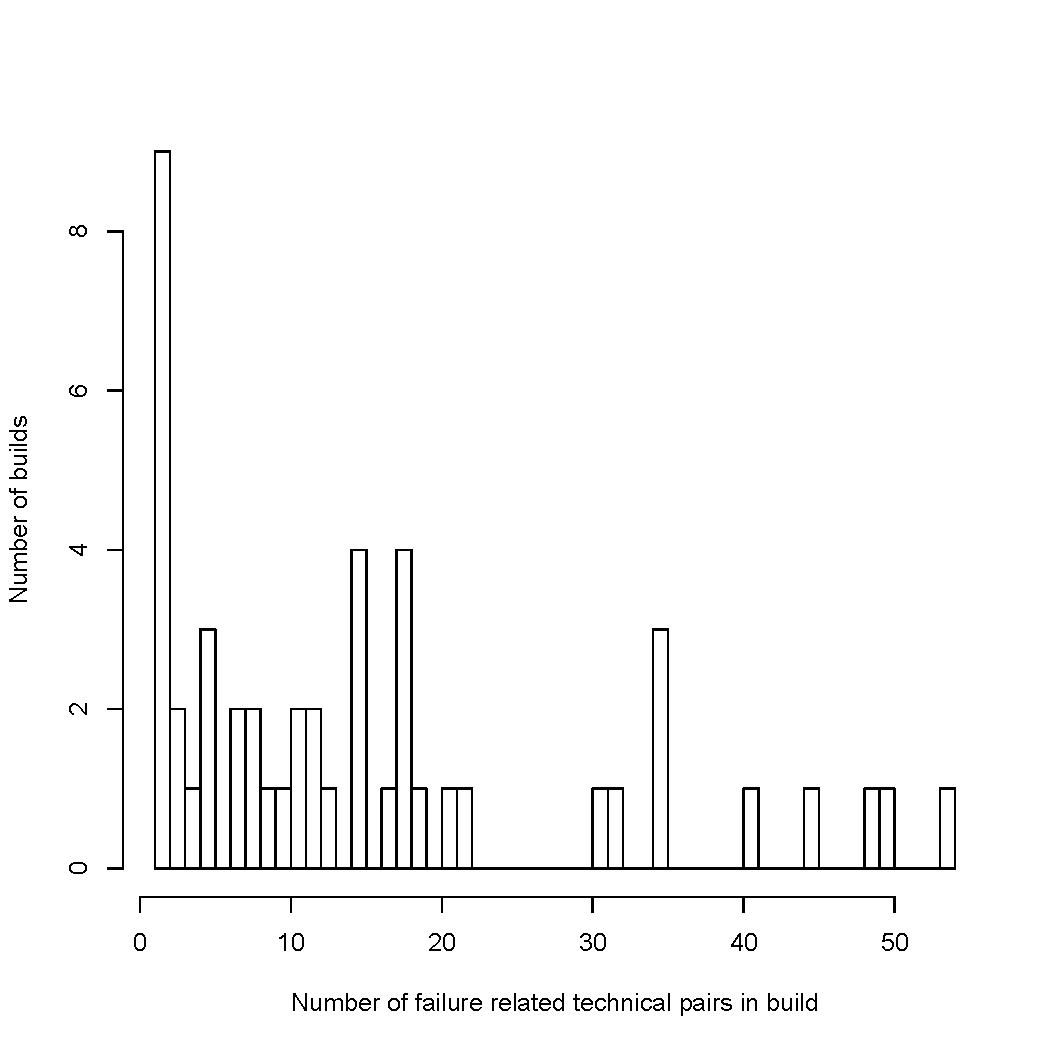
\includegraphics[width=\columnwidth]{figures/builddistribution}
\vspace{-.75cm}
\caption{Histogram of how many builds have a certain number of failure-reated technical pairs.}
\label{fig:builddistribution}
\end{figure}

\subsection{Discussion}
\label{ch8:dis}
These results show that there is a strong relationship between certain technical
developer pairs and increased likelihood of a build failure.
Out of the total of 120 technical pairs that increase the likelihood of a
build to fail, only 23 had an existing
corresponding socio-technical pair. Of these, none were statistically
related to build failure. This means that 97 pairs of developers that had a
technical dependency did not communicate with each other and
consequently increased the likelihood of a build failure. Our results not only
corroborate past findings~\cite{cataldo:cscw:2006,cataldo:esem:2008} that socio-technical gaps
have a negative effect in software development. More importantly, they indicate
that the analysis presented in this paper is able to identify the specific
socio-technical gaps, namely the actual developer pairs where the gaps occur
and that increase the likelihood of build failure. 

A preliminary analysis of developers membership to teams shows that most
of the technical pairs related to build failure consist of developer belonging to
different teams. Naggappan et al~\cite{nagappan:icse:2008} found that using the
organizational distance between people predicts failures. They reasoned that this
is due to the lack of awareness what people separated by organizational distance
work on. Although the Rational Team Concert team strongly emphasizes communication
regardless of team boundaries, it still seems that organizational distance has
an influence on its communication behaviour.


Although the analysis of technical pairs in relation to build failures
showed that they have a negative influence on the build result, it does not take
into account possible confounding variables. The question is if there developer pairs still effect the build outcome in the presence of confounding variables, such as number of developers involved in a build, number of work items
related to a build, number of change sets per build, and number of files changed.
We tested this using a logistical regression model including both developer pairs and confounding variables.

Overall the logistic regression confirms the effect of the developer pairs
even in the presence of confounding variables, such as number of files changed
and numbers of developers (AIC of 706). 
Table~\ref{tab:regression} shows an excerpt from the complete logistical
regression which shows that the twenty pairs previously identified are still
significant under the influence of the four confounding variables. Because we have 2872 developer pairs, space constraints prevent us from reporting the entire regression model. We chose to report on the coefficients for the twenty pairs that we reported in Table~\ref{tab:regression} as well as the coefficients for the four control features.

All features shown in Table~\ref{tab:regression} are significant at the $\alpha=.001$ level (indicated by the p-value and ***).
We checked for all the other technical pairs that were reported significant using the approach described in the previous section and found that they are all significant in the regression model as well.
Moreover, the four control variables of number of developers per build, number
of work items per build, number of change sets per build, and number of files changed per build are also significant.

Since we model failed builds with 0 and successful builds with 1, a negative coefficient means that the feature increases the chances of a failure.
All pairs reported in Table~\ref{tab:regression} and the technical pairs that we identified to be related to build failure have a negative coefficient.
 


\subsection{Conclusions}
\label{sec:8:conclusions}
We end this chapter by bringing it back to the initial research question we set out to answer:
\begin{itemize}
  \item\textbf{RQ 2.1:} Can Socio-Technical-Networks be manipulated to increase build success? 
\end{itemize}

The results we presented in Section~\ref{ch:fse:result2} show that there are developer pairs with unmet coordination needs that negatively influence build success.
Furthermore, we showed that the corresponding developer pair that fulfills its coordination need is less likely to be associated with build failure and thus theoretically decreasing the likelihood of build failure.
To put it in perspective if any of the twenty most harmful patterns is present in a build the build had at least an 74\% chance to fail.

Besides the technical side of the approach to generate statistically relevant recommendations as Murphy and Murphy-Hill~\cite{murphy:rsse:2010} pointed out developers need to accept such recommendation for them to be ultimately useful.

%% !TEX root = thesis-journal.tex
\section{Acceptability of Recommendations}
\label{chap:talk}
Knowing that our approach can generate statistically significant recommendations is only one necessary step towards showing its usefulness.
As Murphy and Murphy-Hill~\cite{murphy:rsse:2010} pointed out recommendation become of little use once developers reject them.
Thus in this chapter we pursue the following research question:

\begin{itemize}
  \item\textbf{RQ 2.2:} Do developers accept recommendations based on software changes to increase build success? 
\end{itemize}

We want developers to communicate as soon as we suspect that otherwise the likelihood for a build to succeed diminishes.
But currently our investigation only took a very technical stance and ignores many other criteria that might be of relevance to developers.
For instance, it is unlikely that every build is of equal importance.
Furthermore, we also think that developers opinion of each other play a role, such as trust and respect.
Therefore, it is important to explore those less technical aspects of developer relationship to gain a better understanding on when to deliver a recommendation.

%% give chapter overview
%In this chapter, we start by detailing the study design that is relevant to exploring our research question (Section~\ref{sec:studydesign}).
%Then, we present the findings we obtained in Section~\ref{sec:findings}.
%We conclude this chapter with offering an answer to our research question and leading into the subsequent Chapter~\ref{chap:actionable} (Section~\ref{sec:conclusions}).


\subsection{Study Design}
\label{sec:studydesign}
We complement our previous analysis of the Rational Team Concert (RTC) development team repositories with rich qualitative data from interviews and observations, considering that much information on a project's lifecycle is not recorded in its repositories~\cite{aranda:icse:2009}. We focused on studying what factors cause a developer to seek information about a change-set, since change-sets are the smallest units of change to a project that directly impact other developers.

Our research question calls for a mixed methods empirical study. Therefore, we collect data about the team's information-seeking behaviour from three different sources.
First, the author of this thesis was embedded in a sub-team of the RTC team as a participant-observer for four months.
Second, we deployed a survey with the entire development team to validate some of the findings from the observations.
Third, we conducted interviews with the developers from one component team to obtain richer information about their communication behaviour.


\subsubsection{Data Collection}
We used a mixed methods approach to answer our research question. We obtained data from three sources: participant observation, a survey, and a set of interviews with RTC team members.

\paragraph{Participant-Observation}
The  author of this thesis joined one of the RTC development sites in Europe for a four-month period in the Fall of 2010. He was involved as an intern with this development team helping with minor bug fixes, feature development, and testing, and thus was in a position to directly participate in the project development and communication activities. Our data collection opportunities were thus much richer than in typical observations conducted over shorter periods of time, or that do not involve active participation in the project.  During his period as a participant-observer, Adrian kept a daily activity log, recording any information of relevance to the communication behaviour of his team.

The observation period coincided with the months prior to a major release and during which the team focused on extensive testing rather than new feature development. As such, the majority of our observations are concerned with activities around testing the integration of RTC with other IBM Rational products, and it offered the experience of collaborating with many developers from different teams and across the remote sites. Finally, in the one month following the release, Adrian also participated in the development of a feature for the upcoming version of the product.

The team in which he was embedded had the responsibility to develop the task management and the planning components of RTC. There were ten developers at the site, including two novices that had recently joined the team and eight experienced developers. The team includes RTC's three senior project management members, who play a major role in planning the entire product's architecture and development.


\begin{table*}[th!]
%\vspace{1pt}
\centering
\subfloat[Process-related items and quotes]{
\footnotesize
\centering
\begin{tabular}{l@{\hspace{7pt}}l@{\hspace{20pt}}r}
\toprule
Survey Items & Interview Quotes (I)/Participant Observation Quotes (O) & Mean Rank\\
\midrule
Release endgame & (O) \emph{``Adrian, in the endgame we only do minimal changes. Is your change minimal?''}& 3.79\\%319\\
To review the change &(I) \emph{``I often lack sufficient understanding of the part of the code I'm reviewing.''}& 5.00\\%311\\
To approve the change &--- & 5.11\\%298\\
Late milestone &--- & 5.14\\%293\\
During iteration endgame &(O) \emph{``Adrian, in the endgame we only do minimal changes. Is your change minimal?''}& 5.42\\%288\\
Obtain a review for the change &(O) \emph{``It is demotivating to get a reject, thus I talk to my reviewer beforehand.''}& 5.55\\%287\\
Obtain an approval for the change &(O) \emph{``I already fixed it, but I  need to convince my team lead to give me approval.''}& 5.72\\%281\\
Related work item has high severity &--- & 6.00\\%246\\
Verify a fix &(I) \emph{``Often I need to ask how I can tell that a change-set actually fixed the bug.''}& 6.37\\%235\\
Topic of work item the change is attached to &--- & 7.64\\%181\\
Priority set by your team lead&--- & 8.55\\%152\\
Role of the committer (e.g. developer) &--- & 9.00\\%145\\
Early in an iteration &(I) \emph{``... there are weeks I sometimes don't talk to my colleagues at all.'''}& 11.24\\%66\\
Early milestone &--- & 12.10\\%60\\%\emph{``''}
\bottomrule
\end{tabular}
\label{tab:sub-process}
}\vspace{0pt}
\subfloat[Developer-related items and quotes]{
\footnotesize
\centering
\begin{tabular}{l@{\hspace{5pt}}l@{\hspace{-11pt}}r}
\toprule
Survey Items & Interview Quotes (I)/Participant Observation Quotes (O) & Mean Rank\\
\midrule
Author is inexperienced &(O) \emph{``Adrian, please put me always as a reviewer on you change-sets.''}& 2.60\\%385\\
Author recently delivered sub-standard work&(I) \emph{``She just changed teams and still needs to get used to this component.''}& 3.04\\%335\\
Author is not up to date with recent events &(I) \emph{``After you return from vacation we ensure you follow new decisions.''}& 3.15\\%329\\ 
You do not know the change-set author &(I) \emph{``I'd be very irritated if someone other than [...] would touch my code.''}& 5.09\\%269\\	
Author is currently working with you &(O) \emph{``We sometimes discuss changes we made to brag about a cool hack.''}& 5.56\\%226\\	
Author part of same feature team &--- & 6.00\\%190\\ 	
Author part of your team &--- & 7.00\\%188\\ 		
Worked with author before &--- & 7.77\\%165\\ 			
Busyness of yourself &(I) \emph{``If I see a problematic change-set, I'll ask for clarifications even if I'm busy.''}& 8.05\\%164\\
Busyness of the author &(I) {\footnotesize\emph{``If I need to know why an author made that change I just contact him.'' [Even if he is busy.]}}& 8.55\\%147\\
Met in person &(I) \emph{``I've worked with him for 5 years now but never even met him.''}& 9.57\\%117\\
Physical location &(O) \emph{``Here, America or Asia, I don't care, I ping them when they are online.''}& 10.14\\%112\\ 
Author is experienced &--- & 11.00\\%93\\ %\emph{``''}		
Author recently delivered high-quality work &--- & 11.09\\%86\\%\emph{``''}
\bottomrule
\end{tabular}
\label{tab:sub-social}
}\vspace{0pt}
\subfloat[Code-change-related items and quotes]{
\footnotesize
\centering
\begin{tabular}{l@{\hspace{0pt}}l@{\hspace{-19pt}}r}
\toprule
Survey Items & Interview Quotes (I)/Participant Observation Quotes (O) & Mean Rank\\
\midrule
Changed API &(O) \emph{``Adrian, why did you change that API?''} [The RTC team avoids changing API.] & 2.84\\%390\\            	
Don't know why code was changed &(O) \emph{``I don't see a reason why you changed that code, you sure you needed to?''}& 3.00\\%348\\ 
Affects frequently used features &(I) \emph{``Before I ok a fix [even to a main feature], I ask if there is a workaround.''} & 4.10\\%325\\ 
Complex code &--- & 4.89\\%289\\	%\emph{``''}
Introduced new functionality &--- & 6.14\\%260\\ %\emph{``''}
Is used by many other methods &(O) {\footnotesize\emph{``Why did you fix this part? The bug is not in this part of the code, it is used and tested a lot.''}}& 6.41\\%240\\ 
Your code was changed &(I) \emph{``I'd be very irritated if someone other than [...] would touch my code.''}& 6.42\\%232\\ 
Stable code was changed &(O) {\footnotesize\emph{``Why did you fix this part? The bug is not in this part of the code, it is used and tested a lot.''}}& 6.62\\%213\\
Change unlocks previously unused code &--- & 7.42\\%192\\ 
A bug fix &--- & 8.61\\%162\\%\emph{``''}	
A re-factoring &(O) {\footnotesize\emph{``I separate a re-factoring from a fix so that people can ask me questions about the fix.''}}& 9.15\\%152\\
Frequently modified code was changed &(I) \emph{``I like to know where the `construction sites' of the project are.''}& 10.35\\%118\\ 
Code is used by few other methods &--- & 10.96\\%94\\ 	
Simple code was changed\phantom{abcdefgheabcdefghe} &--- & 12.57\\%58\\   %23 characters	43
%Author recently delivered high-quality work	
\bottomrule
\end{tabular}
\label{tab:sub-technical}
}
%\vspace{-10pt}
\caption{This table (in three parts) summarizes the data we collected from our three data sources: 1.) our participant-observer's log-book; 2.) survey responses from 36 developers situated around the world; 3.) interviews with 10 developers.  These items are ranked by their average rank.  Whenever possible, we provided quotes from interviews (I), or quotes from the participant-observation period (O) to exemplify the items.}
%\addtocounter{table}{-1}
\label{tab:surveyfactors}
\end{table*}

\paragraph{Interviews}
We conducted interviews with ten developers of the RTC team to inform our observational findings. The setting for the interviews was slightly unusual, and beneficial from a research perspective, since the first author's participant-observation allowed him to develop working relationships during his stay at the team, and to delve into a discussion of complex communication issues without needing to spend time understanding the basic context of the team.

In the interviews, we requested developers to provide details into their communication dynamics through a narration of ``war stories'' that directly related to communication among developers. ``\emph{War stories}'' are events that left an impression on the respondent. War stories emphasize specific events that they witnessed or took part in~\cite{lutters:ist:2007}; their narrative is particularly powerful at uncovering the elements of the stories that are relevant to the respondents. The interviews lasted between thirty minutes and one hour, and they were conducted at the end of the observation period. 


\paragraph{Survey}
To complement the insights we obtained from the observations and interviews, we deployed a survey with the entire RTC team at the end of our observation period. The survey was designed iteratively and piloted with a European team, and intended to collect input about which factors increase the likelihood of a developer requesting information about a change-set from the change-set author. The items we included in the survey were in the categories of code-related, developer-related and process-related items. Each category included 14 items, as shown in Table~\ref{tab:surveyfactors}. \emph{Code-change related} items describe the change-set delivered or the code that the change-set modifies or affects. \emph{Developer-related} items relate to
the developers that delivered a change-set, the developer requesting the
information, and their relation to each other. Finally, \emph{process-related} items relate to the development phase in effect when the change-set was delivered, and to items relating to process requirements or practices. For each of the three categories, the survey asked the developers to rank each item in the category according to how strongly it increases their likelihood of requesting information about a change-set. 

We initially formulated our list of items from an analysis of the current literature on coordination and communication, as well as from our own previous research. We then refined the list of items through piloting and discussions with the development team. An initial version of the survey included fifty-nine items; the refined list had forty-two. Besides reducing the number of items in our list, the pilot survey led us to add several process-related items, as well as to change the format of the question (the initial survey had a battery of questions with Likert-scale answers; the final survey asked respondents to rank each item in comparison to the rest in its own category).

We deployed the survey through a web form, and invited the entire distributed RTC development team to participate. We sent a reminder one month later to increase the response rate. We obtained 36 responses to the survey; approximately a 25\% response rate.
Of the 36 respondents, 26 are located in North America, 5 are located in Europe, and 5 are located in Asia. Furthermore, 22 of the respondents are developers, 5 team leads, 5 component leads and project management committee, and 4 respondents withheld their information.

\subsubsection{Analysis} 
For our data analysis, we transcribed the interviews, and then coded both the interviews and the participant-observation notes. From the codes we created categories, which we cross-referenced to the survey rankings. We used an open coding approach, during which we assigned codes to summarize incidents in sentences and paragraphs of the transcribed interviews that relate to our research question.

We calculated the ranking of the survey items for each category by calculating the mean over all ranks given by developers to a survey item (see Table~\ref{tab:surveyfactors}).
Table~\ref{tab:sparkle} shows the distribution of the rankings for each survey item.

During our analysis, we derived a set of factors affecting communication behaviour based on our list of survey items and qualitative data from our interviews and observations. Whenever possible, we triangulated our findings using all our data sources. We tried to ensure that all of our findings were supported by at least two data sources; none of the findings we report were challenged by any of our data sources. 


\subsection{Findings}
\label{sec:findings}
The evidence collected from our survey, interviews, and participant observation allowed us to derive seven factors that affect communication behaviour in software organizations, which we outline below. In the remainder of this section, text in italics refers to survey items that can be found in Table \ref{tab:surveyfactors}. Text in italics and around quotation marks denotes interview fragments.

\begin{figure*}[tb]
\centering
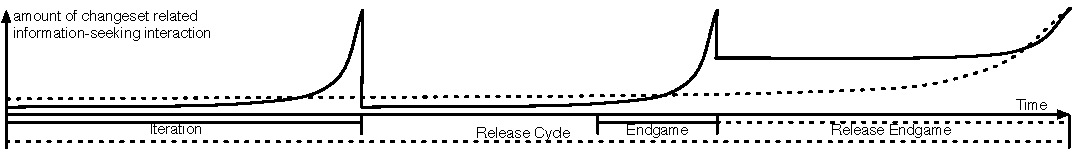
\includegraphics[width=\textwidth]{figures/findingProcess2}
\vspace{-20pt}\caption{The pattern of information-seeking interactions throughout several iterations of a release cycle. Every release cycle consists of a number of iterations; each iteration includes an endgame phase. change-set-based interactions are more frequent during endgame phases and during the last iteration of the release cycle.}
\label{IterationsFig}
\end{figure*}



\addtocounter{table}{1}
\begin{table}[t!]
\centering
\begin{tabular}{ll}
\toprule
\vspace{-2pt}& Process-related items\\
\midrule
\vspace{-2pt}\includegraphics[height=10px, width=30px]{figures/sparkles/during-release-endgame.pdf} & Release endgame\\
\vspace{-2pt}\includegraphics[height=10px, width=30px]{figures/sparkles/you-need-to-review-a-change.pdf} & To review the change\\
\vspace{-2pt}\includegraphics[height=10px, width=30px]{figures/sparkles/you-need-to-approve-a-change.pdf} & To approve the change\\
\vspace{-2pt}\includegraphics[height=10px, width=30px]{figures/sparkles/late-milestone.pdf} & Late milestone\\
\vspace{-2pt}\includegraphics[height=10px, width=30px]{figures/sparkles/during-iteration-endgame.pdf} & During iteration endgame\\
\vspace{-2pt}\includegraphics[height=10px, width=30px]{figures/sparkles/you-need-a-review-for-a-change.pdf} & Obtain a review for the change\\
\vspace{-2pt}\includegraphics[height=10px, width=30px]{figures/sparkles/you-need-an-approval-for-a-change.pdf} & Obtain an approval for the change\\
\vspace{-2pt}\includegraphics[height=10px, width=30px]{figures/sparkles/related-work-item-has-high-severity.pdf} & Related work item has high severity\\
\vspace{-2pt}\includegraphics[height=10px, width=30px]{figures/sparkles/you-need-to-verify-a-fix.pdf} & Verify a fix\\
\vspace{-2pt}\includegraphics[height=10px, width=30px]{figures/sparkles/topic-of-work-item-the-change-is-attached-to.pdf} & Topic of work item the change is attached to\\ 
\vspace{-2pt}\includegraphics[height=10px, width=30px]{figures/sparkles/priority-of-related-work-item-was-set-from-your-team-lead.pdf} & Priority set by your team lead\\
\vspace{-2pt}\includegraphics[height=10px, width=30px]{figures/sparkles/role-of-committer--e-g--developer--team-lead--intern.pdf} & Role of the committer (e.g. developer)\\
\vspace{-2pt}\includegraphics[height=10px, width=30px]{figures/sparkles/early-in-an-iteration.pdf} & Early in an iteration\\
\vspace{-2pt}\includegraphics[height=10px, width=30px]{figures/sparkles/early-milestone.pdf} & Early milestone\\
\midrule
\vspace{-2pt}& Developer-related items\\
\midrule
\vspace{-2pt}\includegraphics[height=10px, width=30px]{figures/sparkles/change-author-is-inexperienced.pdf} & Author is inexperienced\\
\vspace{-2pt}\includegraphics[height=10px, width=30px]{figures/sparkles/recent-work-of-low-quality.pdf} & Author recently delivered sub-standard work\\
\vspace{-2pt}\includegraphics[height=10px, width=30px]{figures/sparkles/change-author-is-not-up-to-date-with-recent-events.pdf} & Author is not up to date with recent events\\
\vspace{-2pt}\includegraphics[height=10px, width=30px]{figures/sparkles/don-t-know-the-change-author.pdf} & You do not know the change-set author \\
\vspace{-2pt}\includegraphics[height=10px, width=30px]{figures/sparkles/currently-working-with-the-change-author.pdf} & Author is currently working with you\\
\vspace{-2pt}\includegraphics[height=10px, width=30px]{figures/sparkles/change-author-part-of-the-same-feature-team.pdf} & Author part of same feature team\\
\vspace{-2pt}\includegraphics[height=10px, width=30px]{figures/sparkles/team-of-change-author.pdf} & Author part of your team\\
\vspace{-2pt}\includegraphics[height=10px, width=30px]{figures/sparkles/worked-with-change-author-in-the-past.pdf} & Worked with author before\\
\vspace{-2pt}\includegraphics[height=10px, width=30px]{figures/sparkles/busyness-of-yourself} & Busyness of yourself\\
\vspace{-2pt}\includegraphics[height=10px, width=30px]{figures/sparkles/busyness-of-the-change-author} & Busyness of the author\\
\vspace{-2pt}\includegraphics[height=10px, width=30px]{figures/sparkles/met-change-author-in-person.pdf} & Met in person\\
\vspace{-2pt}\includegraphics[height=10px, width=30px]{figures/sparkles/physical-location-of-the-change-author.pdf} & Physical location\\
\vspace{-2pt}\includegraphics[height=10px, width=30px]{figures/sparkles/change-author-is-experienced.pdf} & Author is experienced\\
\vspace{-2pt}\includegraphics[height=10px, width=30px]{figures/sparkles/recent-work-of-high-quality.pdf} & Author recently delivered high-quality work\\
\midrule
\vspace{-2pt}& Code-change related items \\
\midrule
\vspace{-2pt}\includegraphics[height=10px, width=30px]{figures/sparkles/change-modified-API.pdf} & Changed API\\
\vspace{-2pt}\includegraphics[height=10px, width=30px]{figures/sparkles/don-t-know-why-code-was-changed.pdf} & Don't know why code was changed\\
\vspace{-2pt}\includegraphics[height=10px, width=30px]{figures/sparkles/code-affects-frequently-used-features.pdf} & Affects frequently used features\\
\vspace{-2pt}\includegraphics[height=10px, width=30px]{figures/sparkles/complex-code-was-changed.pdf} & Complex code\\
\vspace{-2pt}\includegraphics[height=10px, width=30px]{figures/sparkles/change-introduced-new-functionality.pdf} & Introduced new functionality\\
\vspace{-2pt}\includegraphics[height=10px, width=30px]{figures/sparkles/code-is-used-by-many-other-methods.pdf} & Is used by many other methods\\
\vspace{-2pt}\includegraphics[height=10px, width=30px]{figures/sparkles/your-code-was-changed.pdf} & Your code was changed \\
\vspace{-2pt}\includegraphics[height=10px, width=30px]{figures/sparkles/stable-code-was-changed.pdf} & Stable code was changed\\
\vspace{-2pt}\includegraphics[height=10px, width=30px]{figures/sparkles/change-unlocks-previously-unused-code.pdf} & Change unlocks previously unused code\\\
\vspace{-2pt}\includegraphics[height=10px, width=30px]{figures/sparkles/change-was-a-bug-fix.pdf} & A bug fix\\	
\vspace{-2pt}\includegraphics[height=10px, width=30px]{figures/sparkles/change-was-a-re-factoring.pdf} & A re-factoring\\ 
\vspace{-2pt}\includegraphics[height=10px, width=30px]{figures/sparkles/frequently-modified-code-was-changed.pdf} & Frequently modified code was changed \\
\vspace{-2pt}\includegraphics[height=10px, width=30px]{figures/sparkles/code-is-used-by-a-few-other-methods.pdf} & Code is used by few other methods\\ 
\vspace{-2pt}\includegraphics[height=10px, width=30px]{figures/sparkles/simple-code-was-changed.pdf} & Simple code was changed\\
\bottomrule
\end{tabular}
\vspace{-5pt}
\caption{This table contains the distribution of ranks for each survey item. The leftmost point of each sparkline represents the amount of respondents that ranked the item first; the rightmost point represents the amount that ranked it last (14th). No survey item received the same rank from more than ten respondents.}
\label{tab:sparkle}
%\vspace{-20pt}
\end{table}


\subsubsection{Development Mode}
One of the strongest findings from our study was the effect of the development mode that the team is in on its communication behaviour. Developers and managers alike give much importance to the development mode they are in, namely (1) normal iteration, and (2) endgame.

The normal iteration mode mainly consists of work that can be planned by the developer. This work tends to be new feature development, or modifications to existing features. Most of the planning for it has been laid out in advance; furthermore, each developer individually knows what features have been assigned to her, and can plan ahead to meet her obligations.
In contrast, the endgame mode mainly consists of work that is coming uncontrollably in short intervals from others. As a result of integration and more intense testing, defects crop up more rapidly and need to be addressed more quickly. Beyond allocating time for endgame activities, there is very little in this development mode that can be planned in advance.

The RTC team switches between the two modes in each iteration. Of the six weeks of a regular iteration, four weeks are assigned to normal iteration mode and two weeks to endgame. However, as deadlines approach, there are occasional special iterations that consist mostly of endgame-like work. In this manner, the same detailed pattern of alternation between normal iteration and endgame within an iteration is reproduced at a higher level, as shown in Figure~\ref{IterationsFig}.

We identified the same pattern with respect to the amount of change-set-related interactions in the team. We found that the mode in which the team is currently in is an important factor determining whether developers will feel a need to communicate about change-sets. Being in endgame mode increases the need for developers to communicate about a change-set, whereas being in normal mode decreases the need to request information about it.

The first author of this paper experienced both modes during his participant-observer time with the RTC team. He joined the team in a release endgame phase, which was characterized by fixing bugs that were reported by testers, and he helped by fixing minor bugs as well as setting up servers for testing. When the team released the project, it switched gears, and in the decompression after the endgame he had the opportunity to develop a feature for the product. The differences in the patterns of interaction between the two modes were distinctly clear, for him and for his peers. During the endgame mode, developers were essentially ``on demand,'' available to fix whatever bugs were discovered. Later, during the normal iteration mode, they experienced far more autonomy and control over their time, and began working on activities that were less demanding of an interaction back-and-forth, and especially less demanding of keeping track of the change-sets committed by their peers. In our interviews, developers almost unanimously pointed to the separation of the two types of modes, describing the differences in the type of communication in each, and identifying the autonomous \emph{vs.}~uncontrollable, inside \emph{vs.}~outside influence.

This is not to say that developers do not communicate while they are in normal iteration  mode, but that the nature of their communication seems to be different. In normal iteration mode, developers communicate less about concrete change-sets, but they communicate more about high level ideas: for instance, they raise questions about how a feature fits into the existing architecture or general tactics to implement a feature, about how much of it actually needs to be implemented or can be reused from other libraries, and so forth. Generally, however, the amount of communication decreases in normal iteration mode. As a developer commented in one of our interviews, \emph{``during feature development iterations there are weeks I sometimes don't talk to my colleagues at all.''} 

In contrast, the endgame mode is characterized by bug reports and last minute feature requests---that is, by work coming into every developer's desk uncontrollably. change-sets become first class concerns during this mode because each change threatens the stability of the product: developers need to evaluate whether the change-set actually improves the product instead of making things worse. Therefore, they develop a habit of reviewing each other's change-sets to assess the risk they pose to the project's stability.

Our survey data provides significant support for this finding. In Table~\ref{tab:sub-process}, we can see that overall, for the RTC development team at large, there is a greater likelihood to request information during product-stabilizing phases, such as 
\emph{during the release endgame}, and a lesser likelihood to request information when working towards an \emph{early milestone}. The former was ranked as the most important of the process-related items in our survey; the latter was ranked as the least important. All the survey items that refer to a late stage in the iteration or in the project lifecycle were ranked highly, and all the items that refer to an early stage were ranked lowly. This finding resonates especially with the team we interviewed. 


\subsubsection{Perceived Knowledge of the change-set Author}
One key determinant for a developer to seek information about a change-set consists of what the developer knows about the background of its author. Several aspects of the author's background seem to be important: the quality of her recent work, her level of experience, and her awareness of recent team events or decisions.

First, these factors are important in part because they point to potential problems with the stability of the product. If a change-set author has \emph{recently delivered sub-standard work}, other developers will want to ensure that the new change-set will not deteriorate their product, and therefore they will try to find more information about it.

Similarly, when the author is \emph{inexperienced}, or is not \emph{up to date} with recent team events for any reason, the risk of introducing problems into the product increases. One developer that interacts frequently with a newly founded team told us that \emph{``most of the work that I need to review is of very low quality and needs several iterations before it is up to our standards.''} Novices, generally speaking, face a ramp-up problem that takes a significant amount of time to overcome~\cite{begel:sigcse:2008}. This was the case with Adrian's work, too: his first change-sets were subjected to more scrutiny due to his unfamiliarity with the code base.

The survey data backs up these observations. The three top items in Table \ref{tab:sub-social} consist of factors related to an unfavourable perception of the background of the change-set author. In comparison, the two least important items in that table refer to favourable perceptions of said background.

In essence, these items point to the relevance of trust in software development teams. For developers, trust in the skills of their colleagues is important. If this trust is not-established (for instance, if a developer does not know the change-set author), developers are more likely to check the change-set and request information to ensure that the modifications were truly necessary and appropriate. But when trust exists (that is, when the author has a good record of delivering high-quality work, or is known to be an experienced team member), the need to seek information about a change-set decreases. 


\subsubsection{Common Experience and Location}
Shared work experiences affect the likelihood of information-seeking behaviour in the RTC distributed team. This is partly related to the trust and perception issues discussed above, but also to the establishment of interpersonal relations and to the intertwining work responsibilities and expectations.

According to our interviews, this is the case particularly for senior team members. Although they work in a globally distributed team, they have managed to establish personal relationships with developers at many different sites. Through continuous interaction and through social events, they have learned more about each other, and thus feel more comfortable to initiate contact with them. Junior team members, in contrast, know very few of their teammates globally, and since they simply do not have these interpersonal connections with the rest of their team, it is less important to them whether they know the author of a change-set when needing to contact them.

Generally speaking, despite the lack of opportunities to build personal relationships with off-site people, for most developers sharing common experiences makes it easier to contact teammates to request information. One team lead told us: \emph{``I have one or two contact people in each team we usually work with whom I ask for information and then often enough get referred to the right person in their team.''}

Our participant-observation data confirm this. At one point, Adrian needed to set up and test a specific component in the RTC product. The development team in charge of that component was located on a different site. However, since Adrian had previously had the opportunity to establish relationships with some of the developers of that team through a previous research study, it was easier for him to contact them and ask for help in his setup task.

Our survey data corroborate these observations. It suggests that the developers that form relationships (on a personal or work level) with other developers gave more emphasis on previous experiences with them. For instance, it made a difference whether the developers \emph{are currently working together} (Table~\ref{tab:sub-social}). Additionally, whether they have shared work experiences seems to be a more determinant factor than having \emph{met in person} or sharing the same \emph{physical location}.

This last finding would seem to indicate that the RTC team has managed to overcome obstacles created by geographical distance. Developers state that the physical location of a change-set author is not an important factor to seek more information about the change-set. Nevertheless, we should note two things. First, this finding merely points out that developers have no greater need to inform themselves of work output of their remote peers than of their local peers; it says nothing about the ease with which such information is acquired. Second, the RTC team has determined to carry out as many of its interactions as possible through textual, electronic media. This neglects the natural advantages provided by proximity in favour of uniform accessibility of interactions, no matter the physical location of the interlocutors.



\subsubsection{Risk Assessment}
A central factor at the heart of the decision to seek information is a concern with the quality of the product and components developed by the team at large. Both managers and developers share this concern. Because of it, every team member is constantly evaluating whether there are significant risks involved in accepting a change-set and including it into the final product. This concern is greatest close to releases or major milestones, and less important when the team is in normal iteration mode.

Developers request information more frequently about change-sets that touch on code that has a high customer impact. According to our interviews and observations, code parts with a high customer impact are those that are directly related to frequently used features or changes to the API that might be used by customers to customize the RTC product. In the case of the impact of API changes, there is an extensive knowledge exchange in the jazz.net forums between customers and developers about how to use the API to build extensions to RTC, which gives developers plenty of information about the possible impact of API changes to the customers. Consequently, change-sets that modify code that has less impact on the customer are of less concern and less likely to be discussed. For example, when scanning fixes to reported bugs, developers perform a risk assessment to determine whether the bug fix is even needed. In the words of one team member, \emph{``with every tenth bug fix you introduce another bug to the system, so unless the bug does not have a workaround and is something most customers would experience, we give it low priority.''}

The ranking of items in Table \ref{tab:sub-technical} provides additional insights into the kinds of change-sets that carry a risk for developers. A \emph{changed API} comes at the top of the list, code that \emph{affects frequently used features} comes third, immediately followed by changes to \emph{complex code}, changes that \emph{introduced new functionality}, and changes to code that \emph{is used by many other methods}.


%\subsubsection{Work Allocation and Peer Reviews}
%In the later stages of the development cycle, developers have two process-based constraints that prompt them to interact with their peers. First, they need their peers to review their change-sets before they are included in the product. Second, they need an approval to start working on a task (a triaging process needs to take place so that developers are allocated to the most important work items).
%
%In the change-set review process, there are two ways the change-set author and the reviewers interact.
%Either the change-set author submits his change-set for review, or the change-set author discusses the change-set with the reviewer before submitting it for review. The main discriminant between meeting with the reviewer to discuss the change-set before submitting it or submitting without prior discussion seems to be whether the reviewer and the author are co-located.
%
%Adrian's mentor during his time with the RTC team explained: \emph{``It is very demotivating to get a change-set rejected, that's why we usually try to discuss things before and then the reviewing just becomes all about quickly testing and accepting the change-set.''} Of course, this does not prevent an already discussed change-set from being rejected, but it signals that the process-based constraint is not as strict as to forbid discussions about a change-set between authors and reviewers in the interest of an unbiased code review.
%
%In the case of developers seeking approval to start working on a task, the process is similarly flexible. The approval is supposed to be issued before the developer begins work on the task. However, we observed several times that developers performed quick fixes, and later went to their team leads to acquire approval for the fixes they had already performed.
%
%Several items in our survey point to the importance of information-seeking around the processes of approval and peer review. In Table \ref{tab:sub-process}, the second- and third-highest items were information needed because the respondent needed \emph{to review the change} or \emph{to approve the change}. The need to  \emph{obtain a review for the change} or to \emph{obtain an approval for the change} were of moderate importance. \emph{Verifying a fix} was not judged as important by our respondents.
%
%\subsubsection{Type of Change}
%The three main reasons for a developer to commit a change-set are to (1) do feature development, (2) fix bugs, and (3) re-factor. Among them, feature development seems to be the one that prompts developers to seek information the most.
%In our survey (Table \ref{tab:sub-process}), code that \emph{introduced new functionality} is ranked fifth among the code-change related factors, while changes that consist of \emph{a bug fix} and \emph{a refactoring} ranked far lower on the same list.
%
%This may be due to the fact that feature development has less tool support than bug fixing (which is supported by debugging tools and automated test frameworks) and refactoring (which is essentially an automatic process today). The limited tool support and the inherently difficult nature of the task itself makes change-sets that introduce new functionality more difficult to understand or assess. Hence, developers are more likely to request information about them.


\subsubsection{Business Goals vs Developers' Pride}
Senior team members (managers and team leads among them) often ask about the purpose and the real need of a change-set in order to minimize unpleasant surprises that might be introduced with further code changes, and simply to have an economically feasible product. One senior development lead told us: \emph{``often I need to stop my developers from fixing every little bug otherwise we would never be able to ship.''}

Although every team member is concerned with the quality of their product, a more realistic, business-oriented perspective seems to be more prominent in the senior team members' information-seeking behaviour: they may request clarifications on the business case of change-sets or work items if they are not immediately clear in the existing documentation.

More junior team members, however, do not have this concern. They express their pride in the actual product and want it to be as bug free as possible. A developer commented to us: \emph{``I want to be proud of what I deliver and I am fairly certain if we don't fix it now it will come back to haunt us because it might upset some customers.''} Not only does this lead the developer to try to convince her manager that including change-sets for seemingly unimportant fixes is valuable, it also makes her information-seeking behaviour different with respect to that of the more senior team members. Broadly speaking, managers will be more interested in seeking clarifications as to the business case of a work item if it is not clear in its description, while developers will not care as much about this.


\subsection{Conclusions}
\label{sec:conclusions}
We end this chapter by bringing it back to the initial research question we set out to answer:
\begin{itemize}
  \item\textbf{RQ 2.2:} Do developers accept recommendations based on software changes to increase build success? 
\end{itemize}

The findings we presented in Section~\ref{sec:findings} show that there are different factors that influence developer to inquire about change-sets.
Although not directly asked for, the developer with reporting on those factors answered our research question in a positive way.
Our approach would provide developers with recommendations either on a per change-set level or while they are working on the code.
We found that developer do talk about change-sets which represent our level of recommendations as well as they show interest in build outcome towards the end of a release cycle.
Thus we can say that the level of our recommendation seems to be appropriate when keeping it to the change-set level.
Examining our finding about risk assessment, which is practices by every lead and developer we are confident that developer would welcome notifications on how risky with respect to build success the changes they are currently applying are to give them a chance to either talk to the recommended person or reconsider the change altogether.
Hence, we are confident the developer answers both validated that they would accept recommendations both in the form we present them, namely per change-set submitted, as well as lending our outcome metric more credibility as they show a keen interest in build success when the date to ship the product approaches.

In the next chapter we return to our path of a more direct analysis of our recommendations by showing a proof of concept that the recommendations do not only statistically relate to build outcome but that recommendation could actually prevent build failures.

\section{Acceptability of Recommendations}
\label{chap:talk}
In this section we present a study that explores to what extend developer would welcome recommendations generated through our approach.
Thus the guiding question for this section is:
\begin{itemize}
\item\textbf{RQ 2.2:} Do developers accept recommendations based on software changes to increase build success? (Section~\ref{chap:talk})
\end{itemize}

By leveraging a combination of a participant observer study with interviews and surveys, we analysed the communication behaviour of a component team within the Rational Team Concert development team.
We compiled a list of findings that detail on what triggered developers to talk to each other about change-sets -- the level of our recommendations.


\subsection{Methodology}
In the three month period in which we joined the development team as an intern developer we kept a detailed logbook.
From that log book we both inferred the foundation of the findings we present.
Furthermore, the log book entries served as the basis for the questionnaire pilot that we run with the local team we were embedded with before  replying the questionnaire with the Rational Team Concert development team at large.

While the Rational Team Concert development team was responding to the questionnaire we interviewed the local team that served as pilot group for the questionnaire

\subsection{Findings}
The four findings we present in this subsection are derived from the three month participant observation period as well as the XXX survey respondents as well as the 10 interviews we conducted with the local development team.

\subsubsection{Development Process}
The Rational Team Concert follows an agile development process that defines 6 week iterations with several iterations forming a release cycle.
Each iteration can be further subdivided into two parts: (1) development and (2) endgame.
The development part os mainly concerned with implementing features and refactoring whereas the endgame is concerned with stabilizing the product.
The endgame period in an iteration gets longer the closer the iteration which translate into a similar pattern on the level of release cycles where iterations close to the end of a release cycle form the release endgame.

Especially during the endgame either in an iteration or towards the end of a release cycle developers show a keen interest in the outcome of the upcoming build.
Because a successful build is important to start using the build themselves while developing developers critically assess changes made to the product to ensure that these changes are not destabilizing the product.
To avoid destabilizing the product developers are continuously coordinating their work and try to ensure that all developers that are effected by their changes are aware of the potential influence.

\subsubsection{Perceived Knowledge of Change Author}
\subsubsection{Common Experience and Location}
\subsubsection{Risk Assessment}


\newpage\ \newpage%\ \newpage
% !TEX root = thesis-journal.tex
%\newpage\ \newpage
\section{Discussion}
\label{chap:disc}
\subsection{An Approach For Improving Social Interactions}
\label{ch:dis:app}
We derived the approach presented in Section~\ref{chap:approach} through two case studies that investigate the usefulness of social and socio-technical networks to predict build outcome (Sections~\ref{chap:soc-net} and~\ref{chap:stc-net2}).
We conducted a study to see if the approach can generate relevant recommendations in Section~\ref{chap:soc-net}.
The study we conducted in the subsequent Section~\ref{chap:talk} further explores the usefulness of the information with respect to whether experts expect the level of recommendations to be of use as well as if these recommendations could be produced in real time and potentially prevent issues from arising.
%The approach we presented in Section~\ref{chap:approach} consists of five steps:
%
%\begin{enumerate}
%\item Define scope of interest.
%\item Define outcome metric.
%\item Build social networks.
%\item Build technical networks.
%\item Generate actionable insights.
%\end{enumerate}

In Section~\ref{chap:soc-net} we showed that the communication structure of a software development team influences build success, suggesting that there is value in manipulating this structure to improve the likelihood for a successful build.
That evidence is further supported by our finding that gaps in the social network constructed from developer communication as suggested by technical dependencies among developers also affect build success (Section~\ref{chap:stc-net2}).

In those two studies we already applied the first four steps of the approach presented in Section~\ref{chap:approach}.
We defined the build as the scope together with the build outcome, success or failure, as the outcome metric.
Using the scope we constructed social networks from the communication among developer that can be related to a build as described in Section~\ref{chap:bg} in both Section~\ref{chap:soc-net} and~\ref{chap:stc-net2}.
Section~\ref{chap:stc-net2} used dependencies among change-set committed by developers that are relevant to a given build to construct a technical network to complement the social network forming a socio-technical network.

In Section~\ref{chap:approach} we showed that we are able to produce recommendations from available repository data that affect build success.
These recommendations take the form of highlighting two developers that have a technical dependency but did not communicate in the context of the build.
%These recommendations in the form of recommending developers to communicate changes the structure of the social network, which we intend in order to improve build success.

We decided to focus on generating recommendation enticing developer to communicate in order improve build success over recommendation that would suggest code changes changing the dependencies among developer for two reasons:
(1) proper code changes are more difficult to suggest without a sufficient understanding of the program requiring more in-depth program analysis and 
(2) developer need to trust the recommendation, which is easier to achieve by limiting ourselves to suggesting people that are affected by a change.

In Section~\ref{chap:talk} we explored the developer view with respect to recommendation systems and if and when recommendation on a change-set level would be appropriate.
The feedback we received generally welcomed such recommendations as long as they are not seen as irrelevant, thus, corroborating Murphy and Murphy-Hill's~\cite{murphy:rsse:2010} point.
Developers, in fact, discuss change-sets in general, but specifically towards the end of a release cycle, as each change becomes more important with respect to the stability of the overall project.

Overall, we gave evidence to the usefulness of our approach by selecting a specific scope and outcome metric, builds and build success respectively, and defined the construction of the social and technical networks in detail (see Section~\ref{chap:bg}).
Furthermore, we showed that the approach can generate actionable insights that are acceptable to developers.
In a final study involving students from two countries we found evidence that we are both able to generate recommendation early enough to be acted upon as well as demonstrated that such recommendation could actually prevent build failures.



\subsection{Implementation Implications}
Besides investigating if developer are open to recommendation that help them prevent build failures our findings from Section~\ref{chap:talk} revealed three implications for the implementation of the approach into a recommendation system.

\subsubsection{Adjust intrusiveness of the notifications}
Our first finding strongly suggests that a developer's information needs can dramatically change between development modes. 
%
When in normal iteration mode, developers act upon planned work and can therefore anticipate the information they need, but in endgame mode, developers react to unplanned incoming work, such as bug reports or requests for code reviews. 

Many tools, such as Codebook~\cite{begel:icse:2010} and Ensemble~\cite{xiang:rsse:2008} provide information and recommendations in a fixed way. 
Codebook enables developers to discover other developers whose code is related.
In contrast,  Ensemble provides a constant stream of potentially relevant events for each developer.
In the Codebook case, this might lead to extra overhead in endgame mode when developers frequently need to search for information instead being automatically provided, whereas Ensemble might overload developers during the feature development mode by providing a constant stream of information.

To avoid overwhelming or to reduce overhead further for developers, recommendation systems should either automatically adjust to the development mode or feature customizable templates that can easily be switched. 

\subsubsection{Group Recommendations}
Our second and third findings unveiled factors that trigger developers to seek information about a change-set that are not related to its code. 
Instead, developers pay close attention to the experience level as well as the quality of previously delivered work to determine whether to talk to the change-set owner.

Traditional recommender systems in software engineering focus on the source code to determine useful recommendations, e.g. Codebook~\cite{begel:icse:2010} and Ensemble~\cite{xiang:rsse:2008}.
This might lead to providing developers with information about changes that are of little interest due to the trust placed in more experienced developer. 

But because developers often look beyond source code and perform an additional step, namely considering the change-set owner's experience and recent work, information solely created from source code might miss interesting instances where novices to the code made inappropriate changes.
Recommender systems might report issues that are of less importance due to the substantial experience of the change-set owner.

Because inferring characteristics of developers can be difficult and asking developers to provide the system with characterizations that change over time, we suggest that implementing a grouping by developers and teams of developer is a good strategy to minimize noise.
This will enable developer to more easily dismiss recommendations pointing to coordinating with certain developers.
 

\subsubsection{Provide Alternative Ranking}
Although the implementation implication we inferred from our second and third finding already yield an alternative ranking that groups together recommendation and ranks those groups, it is still passed on our proposed measure for ranking.
The fourth finding we reported on highlights the interest of developer in the risk that is posed by a change.
Our approach to generate recommendation currently does not consider there change other than to indicate technical dependencies among developers.

To better support developers in their tasks we should provide alternative rankings that take into account other activities such as risk assessment or code-reviews.
Thus an implementation of the approach should not only focus on providing the information that is relevant to the recommendation but also include metrics that developer relied on beforehand, such as number of files changed or which files have been changed.

Providing developer with metrics that they are familiar with serves two purposes:
(1) By providing metrics that are already used in making decision we can entice the developers to use the recommendation system and
(2) by providing known metrics we build trust into the recommendation system, which as highlighted by Murphy et al~\cite{murphy:rsse:2010}.

%\subsection{Contributions through Empirical Studies}
%\label{sec:cont:emp}
%Each study by itself contributed to the overall body of knowledge of software development team coordination.
%We present in the order of our five research questions the contribution of each  study.
%
%
%\subsubsection{Using Build Success as Communication Quality Indicator}
%\label{subsec:practicalimpl}
%%With this study we gave empirical evidence of communication among software developers influencing software quality.
%%Although by itself not surprising that issues in communication can hinder productivity and introduce ambiguities that might lead to problems with respect to software quality, it is, to the best of our knowledge, the first study that instead of looking into content of individual  conversations takes a higher level approach and relates communication structures to software quality.
%%
%We started our investigation by exploring whether there exists a relationship between build success and communication by using prediction models (Section~\ref{chap:soc-net}).
%Our models can be used by Jazz teams to assess the quality of their current
%communication in relation to the result of their upcoming integration. If a team
%is currently working on a component and an integration build is planned in the
%near future, the measures of the current communication in the team can be
%provided as input to our prediction model and the model will predict whether the
%build will fail with a precision shown in Table~\ref{tab:PredictionResultTable}.
%For example, if team P is working towards a build and our model predicts that the
%structure of its current communication leads to a failed build, the team can have
%a 76\% (see Section~\ref{chap:soc-net} Table~\ref{tab:PredictionResultTable}) confidence that the build is
%going to fail. This information can be used by developers in monitoring their
%team communication behaviour, or by management in decisions with respect to
%adjusting collaborative tools or processes towards improving the integration.
%
%\subsubsection{Unmet Coordination Needs Matter}
%% stc and build success
%The relationship between communication structure and build failures however significant has only a small effect on the overall success rate of software builds, the outcome metric we studied.
%This lead us to include information about the system by adding technical dependencies as expressed by the source code among software developers.
%Backed up by findings in the research area of socio-technical congruence we hypothesized that the technical relationships help to zero in onto the important relationships among developers that relate to build failures.
%As the relationship between socio-technical congruence and productivity suggested influence on software quality, we showed in Section~\ref{chap:stc-net2} that it actually predicts build failures with varying accuracy depending on the type of build.
%Thus not meeting coordination needs as demanded by technical dependencies among software developers has a negative effect on build success.
%
%\subsubsection{Developers That Induce Build Failures}
%\label{sec:implications}
%% failure inducing pairs
%Being able to predict whether a build fails already helps developers to plan ahead with respect to future work, such as stabilizing the system in contrast to working on new features, but ultimately we want to be able to prevent builds from failing.
%To that purpose we need to influence the socio-technical network such that it takes a structure that is more favourable to build success.
%We found that certain constellations within a socio-technical network, to be more precise pairings of software developer and their respective relationship, seem to be correlating with build success (Section~\ref{chap:approach}).
%This evidence can be used to recommend action before the build is commenced in the sense that developers can investigate their relationship by for example discussing the code changes that created a technical relationship between them.
%
%Thus, our findings have several implications for the design of collaborative systems.
%By automating the analyses presented here we can incorporate the knowledge about
%developer pairs that tend to be failure related in a real-time recommender
%system. Not only do we provide the recommendations that matter to the upcoming
%build, we also provide incentives to motivate developers to talk about their
%technical dependencies. 
%Such a recommender system can use project historical data to
%calculate the likelihood that an upcoming build fails given a particular
%developer pair that worked on that build without communicating to each other.
%
%For management, such a recommender system can provide details about the
%individual developers in, and properties of, these potentially problematic
%developer pairs. Individual developers may be an explanation for the behaviour of
%the pairs we found in Rational Team Concert. This may indicate developers that are
%harder to work with or too busy to coordinate appropriately, prompting management
%to reorganize teams and workloads. This would minimize the likelihood of a build
%to fail, by removing the underlying cause of a pair to be failure related.
%Similarly, as another example from our study, most developer pairs
%consisted of developers that were part of different teams. In such
%situations management may decide to investigate reasons for coordination
%problems that include factors such as geographical or functional distance in the project.

%\subsubsection{Recommender System Design Guidelines}
%\label{sec:sub:tools}
%% talk or not to talk
%In our first qualitative study (Section~\ref{chap:talk}) we explored whether developers would accept recommendations produced by our approach.
%It turns out, that developers are generally open to recommendations on a low level, such as on a change-set basis, but it depends on external factors such as the development process.
%For instance, we found depending on how close a development team to a software release is the more they focus on the implications of individual changes, whereas developers focus more high level reusability issues at the beginning of a release cycle.
%
%%Nakakoji et al~\cite{nakakoji2010:rdc} formulated nine design guidelines for systems that support seeking information in software teams. Some of them deal with minimizing the interruptions experienced by the developers who are asked for information, while others refer to enabling the information-seeker to contact the right people. Our findings help us refine Nakakoji et al guidelines:
%
%\paragraph{Guideline \#1} \emph{Recommender systems should adjust to the development mode.}
%Our first finding strongly suggests that a developer's information needs can dramatically change between development modes. 
%%
%When in normal iteration mode, developers act upon planned work and can therefore anticipate the information they need, but in endgame mode, developers react to unplanned incoming work, such as bug reports or requests for code reviews. 
%
%%Many tools, such as Codebook~\cite{begel:icse:2010} and Ensemble~\cite{xiang:rsse:2008} provide information and recommendations in a fixed way. 
%%Codebook enables developers to discover other developers whose code is related.
%%In contrast,  Ensemble provides a constant stream of potentially relevant events for each developer.
%%In the Codebook case, this might lead to extra overhead in endgame mode when developers frequently need to search for information instead being automatically provided, whereas Ensemble might overload developers during the feature development mode by providing a constant stream of information.
%%
%%To avoid overwhelming or reducing overhead further for developers, recommendation systems should either automatically adjust to the development mode or feature customizable templates that can easily be switched. 
%
%\paragraph{Guideline \#2} \emph{Recommender systems should account for perceived knowledge of other developers.}
%Our second and third findings unveiled factors that trigger developers to seek information about a change-set that are not related to its code. 
%Instead, developers pay close attention to the experience level as well as the quality of previously delivered work to determine whether to talk to the change-set owner.
%%
%%Traditional recommender systems in software engineering focus on the source code to determine useful recommendations, e.g. Codebook~\cite{begel:icse:2010} and Ensemble~\cite{xiang:rsse:2008}.
%%This might lead to providing developers with information about changes that are of little interest due to the trust placed in more experienced developer. 
%%
%%But because developers often look beyond source code and perform an additional step, namely considering the change-set owner's experience and recent work, information solely created from source code might miss interesting instances where novices to the code made inappropriate changes.
%%Recommender systems might report issues that are of less importance due to the substantial experience of the change-set owner.
%%
%Implementing filtering mechanisms based on author characteristics such as experience and quality of previously delivered work can help developers focus on the information that is important to them.
%
%
%\paragraph{Guideline \#3} \emph{Recommender systems should assist in non-implementation tasks such as code reviews and risk assessment.} 
%We observed, as described in the fourth, fifth, and sixth findings, that developers are highly engaged in discussions when performing risk assessments or reviews of change-sets. 
%
%%In software engineering, most recommendations are focused on providing information to support concrete tasks such as bug fixes or re-factorings, but not for tasks such as reviews. To provide information for non coding tasks, recommender systems should be configurable to display relevant information beyond the tasks that they are intended to support, so that developer can easily access the information provided by recommender systems when performing code reviews or risk assessments.
%
%\paragraph{Guideline \#4} \emph{Recommender systems should account for business goals.}
%Our last finding points to internal conflicts within teams and among developers caused by the desire to create a flawless product under the restriction of a set of business goals such as shipping the product on time.
%%Thus, developers often need to be reminded that they must focus their efforts on fulfilling business goals rather than on polishing the product as they see fit. Existing recommenders that use code-related metrics such as quality or productivity may shift attention away from fulfilling business goals.
%%
%To support developers to focus on business goals, systems supporting the information-seeking behaviour of developers should be able to prioritize information related to tasks that are mission-critical to the organization, helping the team focus its attention on the most relevant problems for the upcoming release.



\section{Threats to Validity}
\label{sec:threat}
In his section we detail the threats to validity of this thesis.

% limited number of studies
\subsection{External Validity}
In part of this work we draw on information from an observational study (Section~\ref{chap:talk}) and studies relying on development repositories (Sections~\ref{chap:soc-net},~\ref{chap:stc-net2}, and~\ref{chap:approach}) that cover two development projects.
Although this limits the generalizability of the findings presented as well as the validity of the inferred approach, we think that the approach still holds merit as the studies that lay the foundation for the validity of generating insights in real time are derived from and industrial project comprising more than one hundred developers at a large software corporation.
This in-depth relationship created by working together with the IBM Rational Team Concert development team limits the amount of data available for the studies we presented but this in-depth relationship enables us to better interpret the collected data as well as gain a deeper understanding of the organization and their processes and how they influence the data.
In the case of the in class study, we aimed to minimize the conclusions we drew to only serve as a feasibility study to demonstrate that technical networks can be constructed in real time as well as give some evidence that potential recommendations can prevented build failures from occurring.

In our close relationship with the IBM Rational Team Concert team we had the chance to interview ten developers, which represent a fraction of the development team at large. These ten developers were all located at the same site. As a result of this, our interview data could be biased and unrepresentative of the RTC team at large.
However, we are confident that this threat is minor, due to the mix of developers we interviewed, including novices, senior developers, and team members that had been part of the group since its beginning.
Furthermore, the triangulation with our observations and survey responses increases our confidence in our findings.

\subsection{Construct Validity}
In this thesis we conceptualized social dependencies among developers using digitally recorded communication artifacts in the form of work item discussions as well as relied on technical dependencies inferred from developers changing the same source code file.
Both constructs are used by the software engineering research community in several studies (e.g.~\cite{cataldo:cscw:2006}).
Nevertheless, both the social and technical dependency characterizations come with the danger that they do not necessary measure social or technical dependencies of relevance or might as well miss existing dependencies.
This leads to the threat that our inferences might be based on inconsistencies in the data such as meaningless communication among developers or file changes that are not technical in nature.
For instance, due to storage problems the Jazz teams erased some build results. In the case of
nightly builds we expected 90 builds (according to project duration) but found
only 15. This might affect our results but we argue that due to our richness of
data the general trend is still preserved.
Given that we use data that was generate by highly disciplined professionals or by students that we monitored we are confident that the data available for analysis is of high quality.

\subsection{Internal Validity}
% never traced found patterns to issues/rellied on statistical analysis
Sections~\ref{chap:stc-net2} and~\ref{chap:approach} demonstrated that constructing the socio-technical networks is feasible and in Section~\ref{chap:approach} we showed that there is a relationship between the network configuration and build success that can be used to generate recommendations.
One issue that we will need to address in future work is showing a definite link between the insights presented in Section~\ref{chap:approach} and the actual build failures and to what extend the recommendations actually can prevent build failures from happening. 
To mitigate this threat we showed some initial evidence of tracing a failed build back to its original failure source and showed that the failure could have been prevented with the socio-technical information available at the point in time when the error was introduced into the code base.

%We conceptualized communication based on comments on work items. Besides
%that, the Jazz team communicates via email, chat, web-based information and
%face-to-face meetings. Based on our observations and conversations with the Jazz
%team, we are certain that comments are mostly used to communicate about work
%items. Since they are work item-specific and immediately available.

Another threat to the approach, which is related to the previously mentioned lack of tracing the basis of the recommendations back to actual build failures, is that we did not test it in the field to see how the recommendation affect the development process.
We presented in Section~\ref{chap:talk} a study that explored if the recommendations are made at an appropriate level of granularity as well as feedback to the usefulness of such recommendations.
Furthermore, the study conducted in a class room setting also suggests that there is value in generating such recommendations.

The surveys we deployed in our qualitative studies (Section~\ref{chap:talk}) survey asked developers to answer closed questions with a pre-defined list of answers which might introduce a bias.
This bias poses a threat to our findings due to the possibility that we were missing important items.
We mitigated it by developing the survey iteratively by piloting and discussing it with one of the development teams to identify the most important items, and by relying on our other two sources of data to triangulate our findings.











\section{Conclusions and Future Work}
\label{ch:dis:con}
We illustrated an approach to leverage the concept of social-technical congruence to generate actionable knowledge.
%This five step approach focuses on defining two key parameters up front:
%(1) Identify 
%
% (1) the scope of interest and (2) the outcome metric of interest.
%The first parameter scope helps with constructing the social networks (the third step) and constructing the technical networks (the fourth step) by supporting the selection of the best data sources.
%The outcome metric guides the analysis to produce actionable knowledge in the form of indicators that positively or negatively influence the outcome metric (step 5). 
%
% future work
The work we presented lends itself to several venues of future work, such as building and testing the recommendation system with several software development teams to study its impact.
A more interesting avenue to pursue is to explore what software architecture can support what kind of communication and organizational structure.
So far, the research around socio-technical congruence is pointing into the direction of changing how software developers coordinate their work, but we propose to return to the original observation Conway made in that the software architecture will change to accommodate the communication structures in an organization.
Therefore, analyzing software architectures with respect to the project properties, such as distribution of the development team or the organizational hierarchy, might yield valuable insight in guiding design decisions of the software product that not only take into account properties to increase the feature richness or maintainability of the software product but is optimal with respect to properties of the organization and the development team in order to increase productivity and quality. 



% Can use something like this to put references on a page
% by themselves when using endfloat and the captionsoff option.
\ifCLASSOPTIONcaptionsoff
  \newpage
\fi



% trigger a \newpage just before the given reference
% number - used to balance the columns on the last page
% adjust value as needed - may need to be readjusted if
% the document is modified later
%\IEEEtriggeratref{8}
% The "triggered" command can be changed if desired:
%\IEEEtriggercmd{\enlargethispage{-5in}}

% references section

% can use a bibliography generated by BibTeX as a .bbl file
% BibTeX documentation can be easily obtained at:
% http://www.ctan.org/tex-archive/biblio/bibtex/contrib/doc/
% The IEEEtran BibTeX style support page is at:
% http://www.michaelshell.org/tex/ieeetran/bibtex/
\bibliographystyle{IEEEtran}
% argument is your BibTeX string definitions and bibliography database(s)
\bibliography{thesis-journal}
%
% <OR> manually copy in the resultant .bbl file
% set second argument of \begin to the number of references
% (used to reserve space for the reference number labels box)
%\begin{thebibliography}{0}
%
%
%\end{thebibliography}

% biography section
% 
% If you have an EPS/PDF photo (graphicx package needed) extra braces are
% needed around the contents of the optional argument to biography to prevent
% the LaTeX parser from getting confused when it sees the complicated
% \includegraphics command within an optional argument. (You could create
% your own custom macro containing the \includegraphics command to make things
% simpler here.)
%\begin{biography}[{\includegraphics[width=1in,height=1.25in,clip,keepaspectratio]{mshell}}]{Michael Shell}
% or if you just want to reserve a space for a photo:

\begin{IEEEbiography}{Adrian Schr{\"o}ter}
Biography text here.
\end{IEEEbiography}

% if you will not have a photo at all:
\begin{IEEEbiography}{Daniela Damian}
Biography text here.
\end{IEEEbiography}


% You can push biographies down or up by placing
% a \vfill before or after them. The appropriate
% use of \vfill depends on what kind of text is
% on the last page and whether or not the columns
% are being equalized.

%\vfill

% Can be used to pull up biographies so that the bottom of the last one
% is flush with the other column.
%\enlargethispage{-5in}



% that's all folks
\end{document}


